\documentclass{article}
\usepackage[utf8]{inputenc}

\title{Interacting Particle Systems Thesis}
\author{Stefan Eng}
\date{2019/2020}

\usepackage{amsthm}
\usepackage{amssymb}
\usepackage{amsmath}
\usepackage{hyperref}
\usepackage{caption}
\usepackage{mathrsfs}
\usepackage{blkarray}
\usepackage{mathtools}
\usepackage{float}

\usepackage{natbib}
\usepackage{graphicx}

\usepackage{tikz}
\usetikzlibrary{calc, automata, chains, arrows, arrows.meta, graphs, graphs.standard, matrix, positioning, scopes}

\makeatletter
\tikzset{join/.code=\tikzset{after node path={%
\ifx\tikzchainprevious\pgfutil@empty\else(\tikzchainprevious)%
edge[every join]#1(\tikzchaincurrent)\fi}}}
\makeatother
\tikzstyle{labeled}=[execute at begin node=$\scriptstyle,
   execute at end node=$]

\theoremstyle{plain}
\newtheorem{theorem}{Theorem}[section]
\newtheorem{example}{Example}[theorem]
\newtheorem{lemma}[theorem]{Lemma}
\newtheorem{prop}[theorem]{Proposition}
\newtheorem{cor}{Corollary}[theorem]

\theoremstyle{definition}
\newtheorem{defn}[theorem]{Definition}
\newtheorem{exercise}{Exercise}

\theoremstyle{remark}
\newtheorem{note}{Note}
\newtheorem*{remark}{Remark}

\numberwithin{equation}{section}

\newcommand{\R}{\mathbb{R}}
\newcommand{\Rs}{\mathcal{R}}
\newcommand{\Gs}{\mathcal{G}}
\newcommand{\Cs}{\mathcal{C}}
\newcommand{\Q}{\mathbb{Q}}
\newcommand{\A}{\mathcal{A}}
\newcommand{\F}{\mathcal{F}}
\newcommand{\E}{\mathcal{E}}
\newcommand{\M}{\mathcal{M}}
\newcommand{\N}{\mathbb{N}}
\newcommand{\Z}{\mathbb{Z}}
\newcommand{\Zs}{{\{0,1\}^\mathbb{Z}}}
\newcommand{\I}{\mathcal{I}}
\newcommand{\D}{\mathcal{D}}
\newcommand{\B}{{\mathcal{B}_{\mathbb{R}}}}
\newcommand{\BU}{{\mathcal{B}_{[0,1]}}}
\newcommand{\loc}{L_{\text{loc}}^1}
\newcommand{\powset}{\mathcal{P}}
\newcommand{\outm}{\mu^{*}}
\newcommand{\cdict}{\Rightarrow\!\Leftarrow}
\newcommand{\Var}{\operatorname {Var}}

% X_1, ..., X_n
\newcommand{\Xn}{\ensuremath{X_1,\ldots,X_n}}
\newcommand{\xn}{\ensuremath{x_1,\ldots,x_n}}

\begin{document}

\maketitle

\tableofcontents

\section{Background}

\subsection{Probability}

\begin{defn}[Geometric Distribution]
$N$ is geometrically distributed with parameter $p \in (0,1]$ if $N$ is a non-negative integer random variable with probability mass function
$$
P(N = n) = (1 - p)^{n - 1} p
$$
for $n \in \{1,2,\ldots\}$.

Unless otherwise specified, in this paper a geometric distribution is assumed to be supported on $\{1,2,\ldots\}$.
\end{defn}

\begin{defn}[Exponential Distribution]
Let $X$ be a random variable.
If $X$ has a probability density function of
$$
f(x) = \begin{cases}
    \lambda e^{-\lambda x} & x > 0\\
    0 & x \leq 0
    \end{cases}
$$
then we say that $X$ is exponentially distributed with rate $\lambda$, denoted as $X \sim \exp(\lambda)$.
\end{defn}

\begin{theorem}\label{thm:exp_x_less_y}
Let $X \sim \exp(\alpha)$ and $Y \sim \exp(\beta)$ be independent random variables.
Then
$$
P(X < Y) = \frac{\alpha}{\alpha + \beta}
$$
\end{theorem}

\begin{proof}
\begin{align*}
    P(X < Y) &= \int_0^\infty P(X < y | Y = y) f_Y(y) dy\\
    &= \int_0^\infty (1 - e^{-\alpha y}) \beta e^{-\beta y} dy\\
    &= \beta \int_0^\infty \left( e^{-\beta y} - e^{-(\alpha + \beta) y}\right) dy\\
    &= \beta \left(\frac{1}{\beta} - \frac{1}{\alpha + \beta}\right)\\
    &= \frac{\alpha}{\alpha + \beta}
\end{align*}
\end{proof}

\begin{theorem}\label{thm:exp_t_cond}
Let $X \sim \exp(\alpha)$ and $Y \sim \exp(\beta)$ be independent random variables with $T = \min(X,Y)$
Then $T \sim \exp(\alpha + \beta)$.
\end{theorem}

\begin{proof}
\begin{align*}
    P(\min(X,Y) > z) &= P(X > z, Y > z)\\
    &= P(X > z) P(Y > z)\\
    &= e^{-\alpha z} e^{-\beta z}\\
    &= e^{-(\alpha + \beta) z}
\end{align*}
So $\min(X,Y) = T \sim \exp(\alpha + \beta)$
\end{proof}

\begin{theorem} \label{thm:exp_scaling}
Let $X \sim \exp(\lambda)$ and $c > 0$ be a constant.
Then $cX \sim \exp(\lambda/c)$.
\end{theorem}

\begin{proof}
$$
    P(cX > y) = P(X > y/c) = e^{-y (\lambda/c)} \quad y > 0
$$
So $cX \sim \exp(\lambda/c)$
\end{proof}

\subsubsection{Generating functions and Characteristic Functions}

\begin{defn}[Probability generating function]
The probability generating function of a discrete random variable $X \in \{0,1,2, \ldots\}$ is defined as
$$
G_X(z) = E[z^X] = \sum_{i = 0}^\infty z^i P(X = i)
$$
for all $z \in \R$ in which the sum converges.
\end{defn}

\begin{note}
For a discrete non-negative integer-valued random variable $X$,
\begin{itemize}
    \item $G_X(0) = P(X = 0)$ since $0^0 = 1$
    \item $G_X(1) = 1$
\end{itemize}
\end{note}

\begin{defn}[Characteristic function]
The characteristic function of a random variable $X$ is the function $\varphi_X : \R \to \mathbb C$ defined as
$$
\varphi_X(t) = E[e^{itX}]
$$
\end{defn}

\begin{remark}
Some properties about the characteristic function
\begin{itemize}
    \item $\varphi_X(0) = 1$
    \item If the $k$th moment exists for $X$ then $\varphi_X$ is $k$ times differentiable and $E[X^k] = i^{-k} \varphi_{X}^{(k)}(0)$
\end{itemize}
\end{remark}

\begin{theorem}[Moments from generating function]
Let $X$ be a discrete random variable on the non-negative integers and $G_X(z)$ be its probability generating function
\begin{itemize}
    \item $E[X] = G'(1)$
    \item $E[X (X - 1) \cdots (X - k + 1)] = G^{(k)}(1)$
\end{itemize}
Provided the derivatives exist.
\end{theorem}

\begin{proof}
See \cite{grimmett2001}
\end{proof}

\begin{theorem}
If $X$ and $Y$ are independent non-negative integer random variables then
$$
G_{X + Y}(z) = G_X(z) G_Y(z)
$$
for $z \in \R$ in which the sums converge.
\end{theorem}

\begin{theorem}
For any independent random variables $X$ and $Y$,
$$
\varphi_{X + Y}(t) = \varphi_X(t) \varphi_Y(t)
$$
for all $t \in \R$.
\end{theorem}

\begin{proof}
See \cite{grimmett2001}
\end{proof}

\begin{theorem}\label{thm:generating_random_sum}
Let $X_1, X_2, \ldots$ be i.i.d random variables with common probability generating function $G_X(z)$.
Let $N$ be another non-negative integer random variable, independent of the sequence $(X_n)$ and $G_N(z) = E[z^N]$ be the probability generating functions for $N$.
Let $S = \sum_{i = 1}^N X_i$.
Then,
$$
G_S(z) = G_N(G_X(z))
$$
\end{theorem}

\begin{proof}
\begin{align*}
    G_X(z) &= E[ z^S ]\\
    &= E[ E[ z^{\sum_{i = 1}^N X_i} | N ]]\\
    &= E \left[ \prod_{i = 1}^N E[z^{X_i}] \right] && \text{by independence}\\
    &= E[ G_X(z)^N]\\
    &= G_N(G_X(z))
\end{align*}
\end{proof}

\begin{theorem}\label{thm:char_func_random_sum}
Let $X_1, X_2, \ldots$ be i.i.d random variables with common characteristic function $\varphi_X(t)$.
Let $N$ be a non-negative integer random variable, independent of the sequence $(X_n)$.
Let $G_N(z) = E[z^N]$ be the probability generating function for $N$.
Let $S = \sum_{i = 1}^N X_i$.
Then,
$$
\varphi_S(t) = E[\varphi_X(t)^N] = G_N(\varphi_X(t))
$$
\end{theorem}

\begin{proof}
\begin{align*}
    \varphi_S(t) &= E[ \exp(it \sum_{i = 1}^N X_i) ]\\
    &= E[ E[ \exp(it \sum_{i = 1}^N X_i) | N ]]\\
    &= E \left[ \prod_{i = 1}^N E[\exp(it X_i)] \right] && \text{by independence}\\
    &= E[\varphi_X(t)^N]\\
    &= G_N(\varphi_X(t))
\end{align*}
\end{proof}

\begin{defn}[Finite mixture]
Let $X_1,\ldots, X_n$ be random variables.
First sample from the random variables according to weights $\alpha = (\alpha_1, \ldots, \alpha_n)$ with $\sum_i \alpha_i = 1$ and $\alpha_i \geq 0$.
Then realize the selected random variable.
This new random variable $X$ is called a \textbf{mixture} of $X_1,\ldots, X_n$.

Let $F_1, \ldots, F_n$ be the corresponding cumulative density functions of $X_1, \ldots, X_n$ and $f_1, \ldots, f_n$ the probability density functions (if they exist).
Then the CDF of $X$ is defined as
$$
F(x) = \sum_{j = 1}^n \alpha_j F_j(x)
$$
and the PDF is defined as
$$
f(x) = \sum_{j = 1}^n \alpha_j F_j(x)
$$
\end{defn}

\begin{defn}[Convolution]
Let $f$ and $g$ be functions. Then, the convolution of $f$ and $g$, denoted $f * g,$ is defined as
$$
(f * g)(z) = \int_{-\infty}^\infty f(t) g(z - t)~dt =  \int_{-\infty}^\infty f(z - t) g(t)~dt
$$
\end{defn}

\begin{theorem}
Let $X$ and $Y$ be independent continuous random variables with density functions $f$ and $g$.

Then the distribution of $Z = X + Y$ has a density function
$$
h(z) = (f * g)(z)
$$
where $*$ is the convolution.

If $X$ and $Y$ are independent integer random variables, then
$$
P(Z = z) = \sum_{k = -\infty}^\infty P(X = k) P(Y = z - k)
$$
\end{theorem}

\subsubsection{Random Sums}

\begin{theorem} \label{thm:geom_sum_exp}
Let $N$ be geometrically distributed ($N \in \{1,2,\ldots\})$ with probability of success $p$ and $X_1,X_2,\ldots$ i.i.d and independent of $N$ with each $X_i$ exponentially distributed with rate $\lambda$.
Then,
$$
S = \sum_{i = i}^N X_i
$$
has an exponential distribution with rate $p \lambda$.
\end{theorem}

\begin{proof}
Let $G_N(z)$ be the probability generating function of $N$ and $\varphi_X(t)$ be the characteristic function of each $X_i$.
It is easy to show that
\begin{align*}
    G_N(z) &= \frac{pz}{1 - (1 - p)z}\\
    \varphi_X(t) &= \frac{\lambda}{\lambda - it}
\end{align*}
Then by Theorem \ref{thm:char_func_random_sum},
\begin{align*}
    \varphi_S(t) &= G_N(\varphi_X(t))\\
    &= \frac{
        p \left( \frac{\lambda}{\lambda - it} \right)
        } {
        1 - (1 - p) \frac{\lambda}{\lambda - it}
        }\\
    &= \frac{
        p \lambda
    } {
        \lambda - it - \lambda + p \lambda
    }\\
    &= \frac{
        p \lambda
    } {
        p \lambda - it
    }
\end{align*}
which is the characteristic function of the exponential distribution with rate $p \lambda$.
\end{proof}

\begin{theorem}[Wald's equation]\label{thm:random_sum_ev}
Let $X_1, X_2, \ldots$ be sequence of i.i.d random variables with finite expectation and $N$ a non-negative integer random variable independent of the sequence $(X_n)$, also with finite expectation.
Let $S = \sum_{i = 1}^N X_i$.
Then,
$$
E[ S ] = E\left[\sum_{i = 1}^N X_i\right] = E[X] E[N]
$$
\end{theorem}

\begin{proof}
Let $G_N(z)$  be the probability generating function for $N$ and $\varphi_X(t)$ be the characteristic function for each $X_i$.
By Theorem \ref{thm:char_func_random_sum}, we have that the characteristic function of $S$ is $\varphi_S(t) = G_N(\varphi_X(t))$.
Hence,
$$
\varphi'_S(t) = G'_N(\varphi_X(t)) \cdot \varphi'_X(t)
$$
It follows that
\begin{align*}
    E[S] &= \varphi'_S(1)\\
    &= i^{-1} G'_N(\varphi_X(0)) \cdot \varphi'_X(0)\\
    &= G'_N(1) [i^{-1} \varphi'_X(0)]   \\
    &= E[N] E[X]
\end{align*}

% The not as elegant way.
%\begin{align*}
%    E\left[ \sum_{i = 1}^N X_i \right] &= E\left[ E\left[ \sum_{i = 1}^N X_i | N\right] \right]\\
%    &= \sum_{n = 1}^\infty E\left[ \sum_{i = 1}^n X_i \right] P(N = n) && N, (X_t) \text{ indep.}\\
%    &= \sum_{n = 1}^\infty \sum_{i = 1}^n E\left[ X_i \right] P(N = n)\\
%    &= E\left[ X_i \right] \sum_{n = 1}^\infty n \cdot P(N = n)\\
%    &= E[X_i] E[N]
%\end{align*}
\end{proof}

\begin{theorem} \label{thm:random_sum_var}
Let $X_1, X_2, \ldots$ be i.i.d random variables and $N$ a non-negative integer random variable independent of ($X_n$).
Then,
$$
\Var\left( \sum_{i = 1}^N X_i \right) = E[N]\Var(X) + (E[X])^2 \Var(N)
$$
\end{theorem}

\begin{proof}
See \cite{Ross97}
\end{proof}

The following is analogous to Theorem \ref{thm:geom_sum_exp} but for discrete geometric sums.

\begin{theorem}\label{thm:geom_sum_geom} (\cite{Nelson1995})
Let $X_1, X_2, \ldots$ be i.i.d geometric random variables ($X_i \in \{1,2,\ldots\})$, with parameters $p$ and $N$ a geometric random variable ($N \in \{1,2,\ldots\})$ with parameter $\alpha$, independent of the sequence $(X_n)$.
Then,
$$
S = \sum_{i = 1}^N X_i
$$
is geometrically distributed with parameter $\alpha p$.
\end{theorem}

\begin{proof}
The probability generating functions for $N$ and each $X_i$ are
\begin{align*}
    G_X(z) &= \frac{p z}{1 - (1 - p)z}\\
    G_{N}(z) &= \frac{\alpha z}{1 - (1 - \alpha)z}
\end{align*}

It follows that
\begin{align*}
    G_S(z) &= G_N(G_X(z))\\
    &= \frac{
    \alpha \left( \frac{p z}{1 - (1 - p)z} \right)
    }{
        1 - (1 - \alpha) \left( \frac{p z}{1 - (1 - p)z} \right)
    }\\
    &= \frac{
        \alpha p z
    }{
        1 - z + pz - pz + \alpha p z
    } \\
    &= \frac{
        \alpha p z
    }{
        1 - (1 - \alpha p) z
    }
\end{align*}
So $S$ is geometrically distributed with parameter $\alpha p$
\end{proof}

\subsubsection{Convergence}

\begin{defn}[Weak convergence]
A sequence of probability measures $(\mu_n)$ \textbf{converges weakly} to $\mu$ (notated as $\mu_n \Rightarrow \mu$) if
$$
\lim_{n \to \infty} \int f d\mu_n = \int f d\mu
$$
for all bounded and continuous functions $f$.
If $F_n$ and $F$ are the CDFs of $\mu_n$ and $F$ then this is equivalent to
$$
\lim_{n \to \infty} F_n(x) = F(x)
$$
for all $x \in \R$ that are continuous for $F$.
\end{defn}

\begin{theorem}
$X_n \Rightarrow X$ iff $E[g(X_n)] \to E[g(X)]$ for all continuous and bounded functions $g$.
\end{theorem}

\begin{theorem}[Convergence together lemma] \label{thm:conv_together_lemma}
If $X_n \Rightarrow X$ and $Y_n \Rightarrow c$, where $c$ is a constant, then $X_n + Y_n \Rightarrow X + c$.
\end{theorem}

\subsection{Stochastic Processes}

\subsubsection{Markov Chains}

\begin{defn}[Discrete Markov chain] \cite{schapira2017}
Let $\{X_n : n \geq 0\}$ be a stochastic process with a finite or countable state space $S$.
Each $X_n$ is a discrete random variable with $X_n \in S$.
Let $\mathscr{F}_n = \sigma\{X_0, X_1, \ldots, X_n\}$ which is the $\sigma$-algebra generated by the process up to time $t$.
The process $(X_n)$ is a discrete-time Markov chain if
$$
P(X_{n + 1} \in B | \mathscr{F}_n) = P(X_{n + 1} \in B | X_n)
$$
for each $B \subset S$.
%$$
%P(X_{n + 1} = y | X_n = x, X_{n - 1} = x_{n - 1}, \ldots, X_0 = x_0) = P(X_{n + 1} = y | X_n = x)
%$$
%for all $n \geq 1$ and $y, x, x_{n-1}, \ldots, x_0 \in S$.
\end{defn}

\begin{defn}[Homogeneous Markov Chain]\cite{grimmett2001}
We say that a discrete-time Markov chain $(X_n)$ with state space $S$ is \textbf{time homogeneous} if
$$
P(X_{n + 1} = j | X_n = i) = P(X_{1} = j | X_0 = i) = \mathbf{P}(i,j) = p_{ij}
$$
$\mathbf{P} = (p_{ij})$ is the $|S| \times |S|$ matrix of transition probabilities
$$
p_{ij} = P(X_{n + 1} = i | X_n = j)
$$

All Markov chains are assumed to be time homogeneous in this thesis unless stated otherwise.
\end{defn}

\begin{remark}
Since for a fixed $i$, $P(i, \cdot)$ is a probability measure then we have that
\begin{itemize}
    \item $p_{ij} \geq 0$ for all $i,j$
    \item $\mathbf{P}$ row sums equal one
    $$
    \sum_{j = 0}^\infty p_{ij} = 1
    $$
    for $i = 0, 1, \ldots$
\end{itemize}
\end{remark}

\begin{defn}[Continuous-time Markov chain] \cite{schapira2017}
Let $(X_t) = \{X(t) : t \in \mathbb T\}$, where $\mathbb T$ is some index set (generally $\mathbb T = [0, \infty)$ represents time), be a stochastic processes with countable state space $S$.
Let $(\mathscr{F}_t)$ be the natural filtration of $(X_t)$, i.e., $\mathscr{F}_t = \sigma\{ X_s : s \leq t \}$.
The process $(X_t)$ is a continuous-time Markov chain if
$$
P(X_{t} \in B | \mathscr{F}_s) = P(X_{t} \in B | X_s)
$$
for all $s < t$ and $B \subset S$.

%Then $(X_t)$ is a continuous-time Markov chain if
%$$
%P(X(t_n) = j | X(t_{n - 1}) = i_{n-1}, \ldots, X(t_1) = i_{1}) %= P(X(t_n) = j | X(t_{n - 1}) = i_{n - 1})
%$$
%for all $t_1, \ldots, t_n \in \mathbb T$, with $t_1 < \cdots < t_n$.
\end{defn}

\begin{defn}[Infinitesimal generator matrix]
The \textbf{infinitesimal generator matrix} (or \textbf{transition rate matrix}) $Q$, of a continuous-time Markov chain $(X_t)$ with countable state space $S$, is an $|S| \times |S|$ matrix.
The element $q_{ij}$ of $Q$ denotes the rate departing from i and arriving in state j.
The diagonal is defined as $q_{ii} = - \sum_{j \not = i} q_{ij}$.
Each $i \not = j, q_{ij} \geq 0$ and the rows sum to zero: $\sum_{j} q_{ij} = 0$ for each $i$.

Assuming the chain is in state $i$ at time $t$, the probability of moving to state $j$ in time $h$ for $h \to 0$ is given by
$$
P(X_{t + h} = j | X_{t} = i) = \begin{cases}
    i \not = j & q_{ij} h + o(h)\\
    i = j & 1 + q_{ii} h + o(h)
\end{cases}
$$
\end{defn}

\begin{defn}[Embedded Markov Chain]
Let $(X_t)$ be a continuous-time Markov chain with infinitesimal generator matrix $Q$ and $Y_n$ be the position of the $n$th jump of the process $(X_t)$ with $Y_0$ the initial state of the chain $(X_t)$.
This discrete-time Markov chain $(Y_n)$ is called the \textbf{embedded} (discrete) Markov chain of the process $(X_t)$.
\end{defn}

\begin{defn}[Absorbing State] \cite{grinstead2003}
Let $(X_n)$ be a discrete-time Markov chain.
A state $x \in \Omega$ is absorbing if and only if $P(x,x) = 1$.

If $(X_t)$ is a continuous-time Markov chain then $i \in \Omega$ is absorbing if and only if $Q(x,x) = 0$.
\end{defn}

\begin{defn}[Absorbing Markov Chain] \cite{grinstead2003}
A Markov chain is absorbing if there is at least one absorbing state and it is possible to reach an absorbing state in a finite number of steps from any state.
\end{defn}

\begin{defn}[Canonical Form] \cite{grinstead2003}
Assume we have an absorbing discrete time Markov chain with $r$ absorbing states and $t$ transient states and  transition matrix $P$.
The canonical form of the transition matrix is
\begin{equation}
    P = \begin{pmatrix}
        B & R\\
        0 & I_{r}
    \end{pmatrix}
\end{equation}

where $B$ is an $t \times t$ matrix of transient states, $R$ is an $t \times r$ matrix of absorbing states and $I_{r}$ is the $r \times r$ identity matrix.
\end{defn}

\begin{theorem}\label{thm:visits_geom}
Let $(X_n)$ be a discrete-time Markov chain with countable state space $S$.
The number of visits to each state is geometrically distributed, with parameter equal to the probability of never returning back to the state.
\end{theorem}

\begin{theorem} \label{thm:fund_exp} \cite{grinstead2003}
For an absorbing Markov chain with $B$ is an $t \times t$ matrix of transient states from the canonical form. Let $N$ be a matrix with the same dimensions as $B$. $N_{ij}$ is the expected number of times the chain is in state j when starting in state i for transient states $i$ and $j$. Then,
\begin{equation}
    N = I + B + B^2 + \cdots = (I - B)^{-1}
\end{equation}
\end{theorem}

\begin{proof}
See \cite{grinstead2003}
\end{proof}

\begin{theorem}\label{thm:mc_projection} \cite{LevinPeresWilmer2006}
Let $(X_n)$ be a discrete-time Markov chain with state space $\Omega$ and transition matrix $P$.
Let $\sim$ be an equivalence relation on $\Omega$ and denote the equivalences classes as $\Omega' = \{[x]: x \in \Omega\}$.

If $x \sim x'$ implies that $P(x,[y]) = P(x', [y])$ (where $P(x,A)$ is probability that the chain moves to one of the states $y \in A$ from $x$) then $([X_n])$  is a Markov chain.
The state space is the equivalence classes $\Omega'$ and transition matrix $P'$ defined as $P'([x],[y]) := P(x, [y])$

We call this new Markov chain $([X_n])$ a projection of $(X_n)$ or that we projected $(X_n)$ onto $([X_n])$.
\end{theorem}

\begin{theorem}\label{thm:x_N_indep}
Assume that we have a continuous-time Markov chain with an embedded discrete-time Markov chain $(Y_n)$.
Let $U_i$ be the waiting time in state $Y_i$.
The sequence of holding times $(U_n)$ is conditionally independent given the sequence of states $(Y_n)$.

Also, each $U_i | (Y_n) \sim \exp(Q(Y_i,Y_i))$
\end{theorem}

The core of the proof is included in the following theorem:

\begin{theorem}
Let $X \sim \exp(\alpha)$ and $Y \sim \exp(\beta)$ be independent random variables with $T = \min(X,Y)$.
Then $T$ is independent of $X < Y$.
\end{theorem}

\begin{proof}
Let $f(x,y)$ be the joint distribution of $X$ and $Y$.
Since $X$ and $Y$ are independent, then $f(x,y) = \alpha \beta e^{-\alpha x} e^{-\beta y}$.
\begin{align*}
    P((T > t) \cap (X < Y)) &= P((X > t) \cap (Y > t) \cap (X < Y))\\
    &= \int_t^\infty \int_t^y f(x,y) dx dy\\
    &= \int_t^\infty \int_t^y \alpha \beta e^{-\alpha x} e^{-\beta y} dx dy\\
    &= \int_t^\infty \beta e^{-\beta y} \left(\int_t^y \alpha e^{-\alpha x} dx \right)  dy\\
    &= \int_t^\infty \beta e^{-\beta y} \left( e^{-\alpha t} - e^{-\alpha y} \right) dy\\
    &= e^{-\alpha t} \int_t^\infty \beta e^{-\beta y} - \beta \int_t^\infty e^{-(\alpha + \beta) y} dy\\
    &= e^{-\alpha t} \int_t^\infty \beta e^{-\beta y} - \frac{\beta}{\alpha + \beta} \int_t^\infty (\alpha + \beta) e^{-(\alpha + \beta) y} dy\\
    &= e^{-(\alpha + \beta) t} - \frac{\beta}{\alpha + \beta} e^{-(\alpha + \beta) t}\\
    &= e^{-(\alpha + \beta) t} \left(1 - \frac{\beta}{\alpha + \beta} \right)\\
    &= \frac{\alpha}{\alpha + \beta} e^{-(\alpha + \beta) t}
\end{align*}
By Theorem \ref{thm:exp_x_less_y}, we have that $P(X < Y) = \frac{\alpha}{\alpha + \beta}$ so
\begin{align*}
    P(T > t | X < Y) &= \frac{P(T > t \cap (X < Y))}{P(X < Y)}\\
    &= e^{-(\alpha + \beta) t}
\end{align*}

%So $T | X < Y$ is an exponential distribution with parameter $\alpha + \beta$
Since both $T | \{X < Y\} \sim \exp(\alpha + \beta)$ and $T \sim \exp(\alpha + \beta)$ then $T$ and $\{X < Y\}$ are independent.
\end{proof}

\begin{theorem}[Forward and backward equations] \cite{grimmett2001}
Assume that we have a CTMC on a finite state space $\Omega$ with $P_t = p_{ij}(t)$ where $p_{ij}(t)$ is the homogeneous transition probability from state $i$ to state $j$ in a time interval of length $t$.

The \textbf{forward equations} are
\begin{equation}
    \label{eq:forward_eqs}
    P_t' = P_t Q
\end{equation}

that is
$$
p_{ij}'(t) = \sum_{k} p_{ik}(t) g_{kj}
$$
for each state $i,j \in \Omega$.

The \textbf{backwards equations} are
\begin{equation}
    \label{eq:backwards_eqs}
    P_t' = Q P_t
\end{equation}
\end{theorem}

\subsubsection{Poisson Processes}

\begin{defn}
A function $f$ is is $o(g(x))$ if 
$$
\lim_{x \to \infty} \frac{f(x)}{g(x)} = 0
$$
\end{defn}

\begin{defn}[Counting process] \cite{Ross_SP_95}
A counting process is a stochastic process $\{N(t), t \geq 0\}$ that represents the number of events occurring up to a time $t$ which has the following properties
\begin{enumerate}
    \item $N(t) \geq 0$
    \item $N(t)$ is integer valued
    \item If $s < t$, then $N(s) \leq N(t)$
    \item If $s < t$, then $N(s) - N(t)$ is the number of events occurring in the interval $(s, t]$.
\end{enumerate}
\end{defn}

\begin{defn}[Independent increments]
Let $(X_t)_{t \in \mathbf T}$ be a stochastic process (with $\mathbf T = \N$ or $\mathbf T = \R^+$).
Then for times $t_0, \ldots, t_n \in \mathbf T$ with $t_0 < \cdots < t_n$ we have that
$$
(X_{t_0}, X_{t_1} - X_{t_0}), (X_{t_2} - X_{t_1}), \ldots, (X_{t_n} - X_{t_{n - 1}})
$$
are independent.
\end{defn}

\begin{defn}[Stationary increments]
A stochastic process $(X_t)_{t \in \mathbf T}$ has stationary if for $s,t \in \mathbf{T}$ with $s \leq t$ then $X_t - X_s$ has the same distribution as $X_{t - s}$
\end{defn}

\begin{defn}[Poisson Process] \cite{Ross_SP_95}
A Poisson process is a counting process $\{N(t), t \geq 0\}$ with rate $\lambda > 0$ if
\begin{enumerate}
    \item $N(0) = 0$
    \item $\{N(t)\}$ has independent increments.
    \item The number of events in any interval of length $t$ has a Poisson distribution with parameter $\lambda t$. That is for $n = 0,1,\ldots$
    $$
    P(N(t + h) - N(h) = n) = P(N(t) = n) = \exp(-\lambda t) \frac{(\lambda t)^n}{n!}
    $$
\end{enumerate}

equivalently

\begin{enumerate}
    \item $N(0) = 0$
    \item $\{N(t)\}$ has independent and stationary increments.
    \item $P(N(h) = 1) = \lambda h + o(h)$
    \item $P(N(h) \geq 2) = o(h)$
\end{enumerate}
\end{defn}

\begin{defn}[Interarrival times] \cite{Ross_SP_95}
Let $\{N(t), t \geq 0\}$ be a Poisson process with rate $\lambda$.
Let $X_1$ be the time for the first event and for $n \geq 1$,
denote $X_n$ as the time between the $(n - 1)$st and the $n$th event.
This sequence is another stochastic process $\{X_n, n \geq 1, n \in \N\}$, called the \textbf{interarrival times}.

The sequence $X_1,X_2, \ldots$ are i.i.d exponential distributed with rate $\lambda$. That is, $P(X_n > t) = e^{-\lambda t}$ for all $n$.
\end{defn}

\begin{defn}[Waiting times] \cite{Ross_SP_95}
Let $\{N(t), t \geq 0\}$ be a Poisson process with rate $\lambda$ with interarrival times $\{X_n\}$.
The waiting time (or arrival time) until the $n$th event is 
$$
T_n  = \sum_{i = 1}^n X_i
$$
for $n \geq 1$.

$S_n$ has a gamma distribution with parameters $n$ and $\lambda$.
\end{defn}

\begin{remark}
For a Poisson process $\{N(t), t \geq 0\}$ the key relationship between the waiting times $T_n$ and $N(t)$ is
$$
N(t) \geq n \text{ iff } T_n \leq t
$$
\end{remark}

\begin{figure}[H]
  \centering
    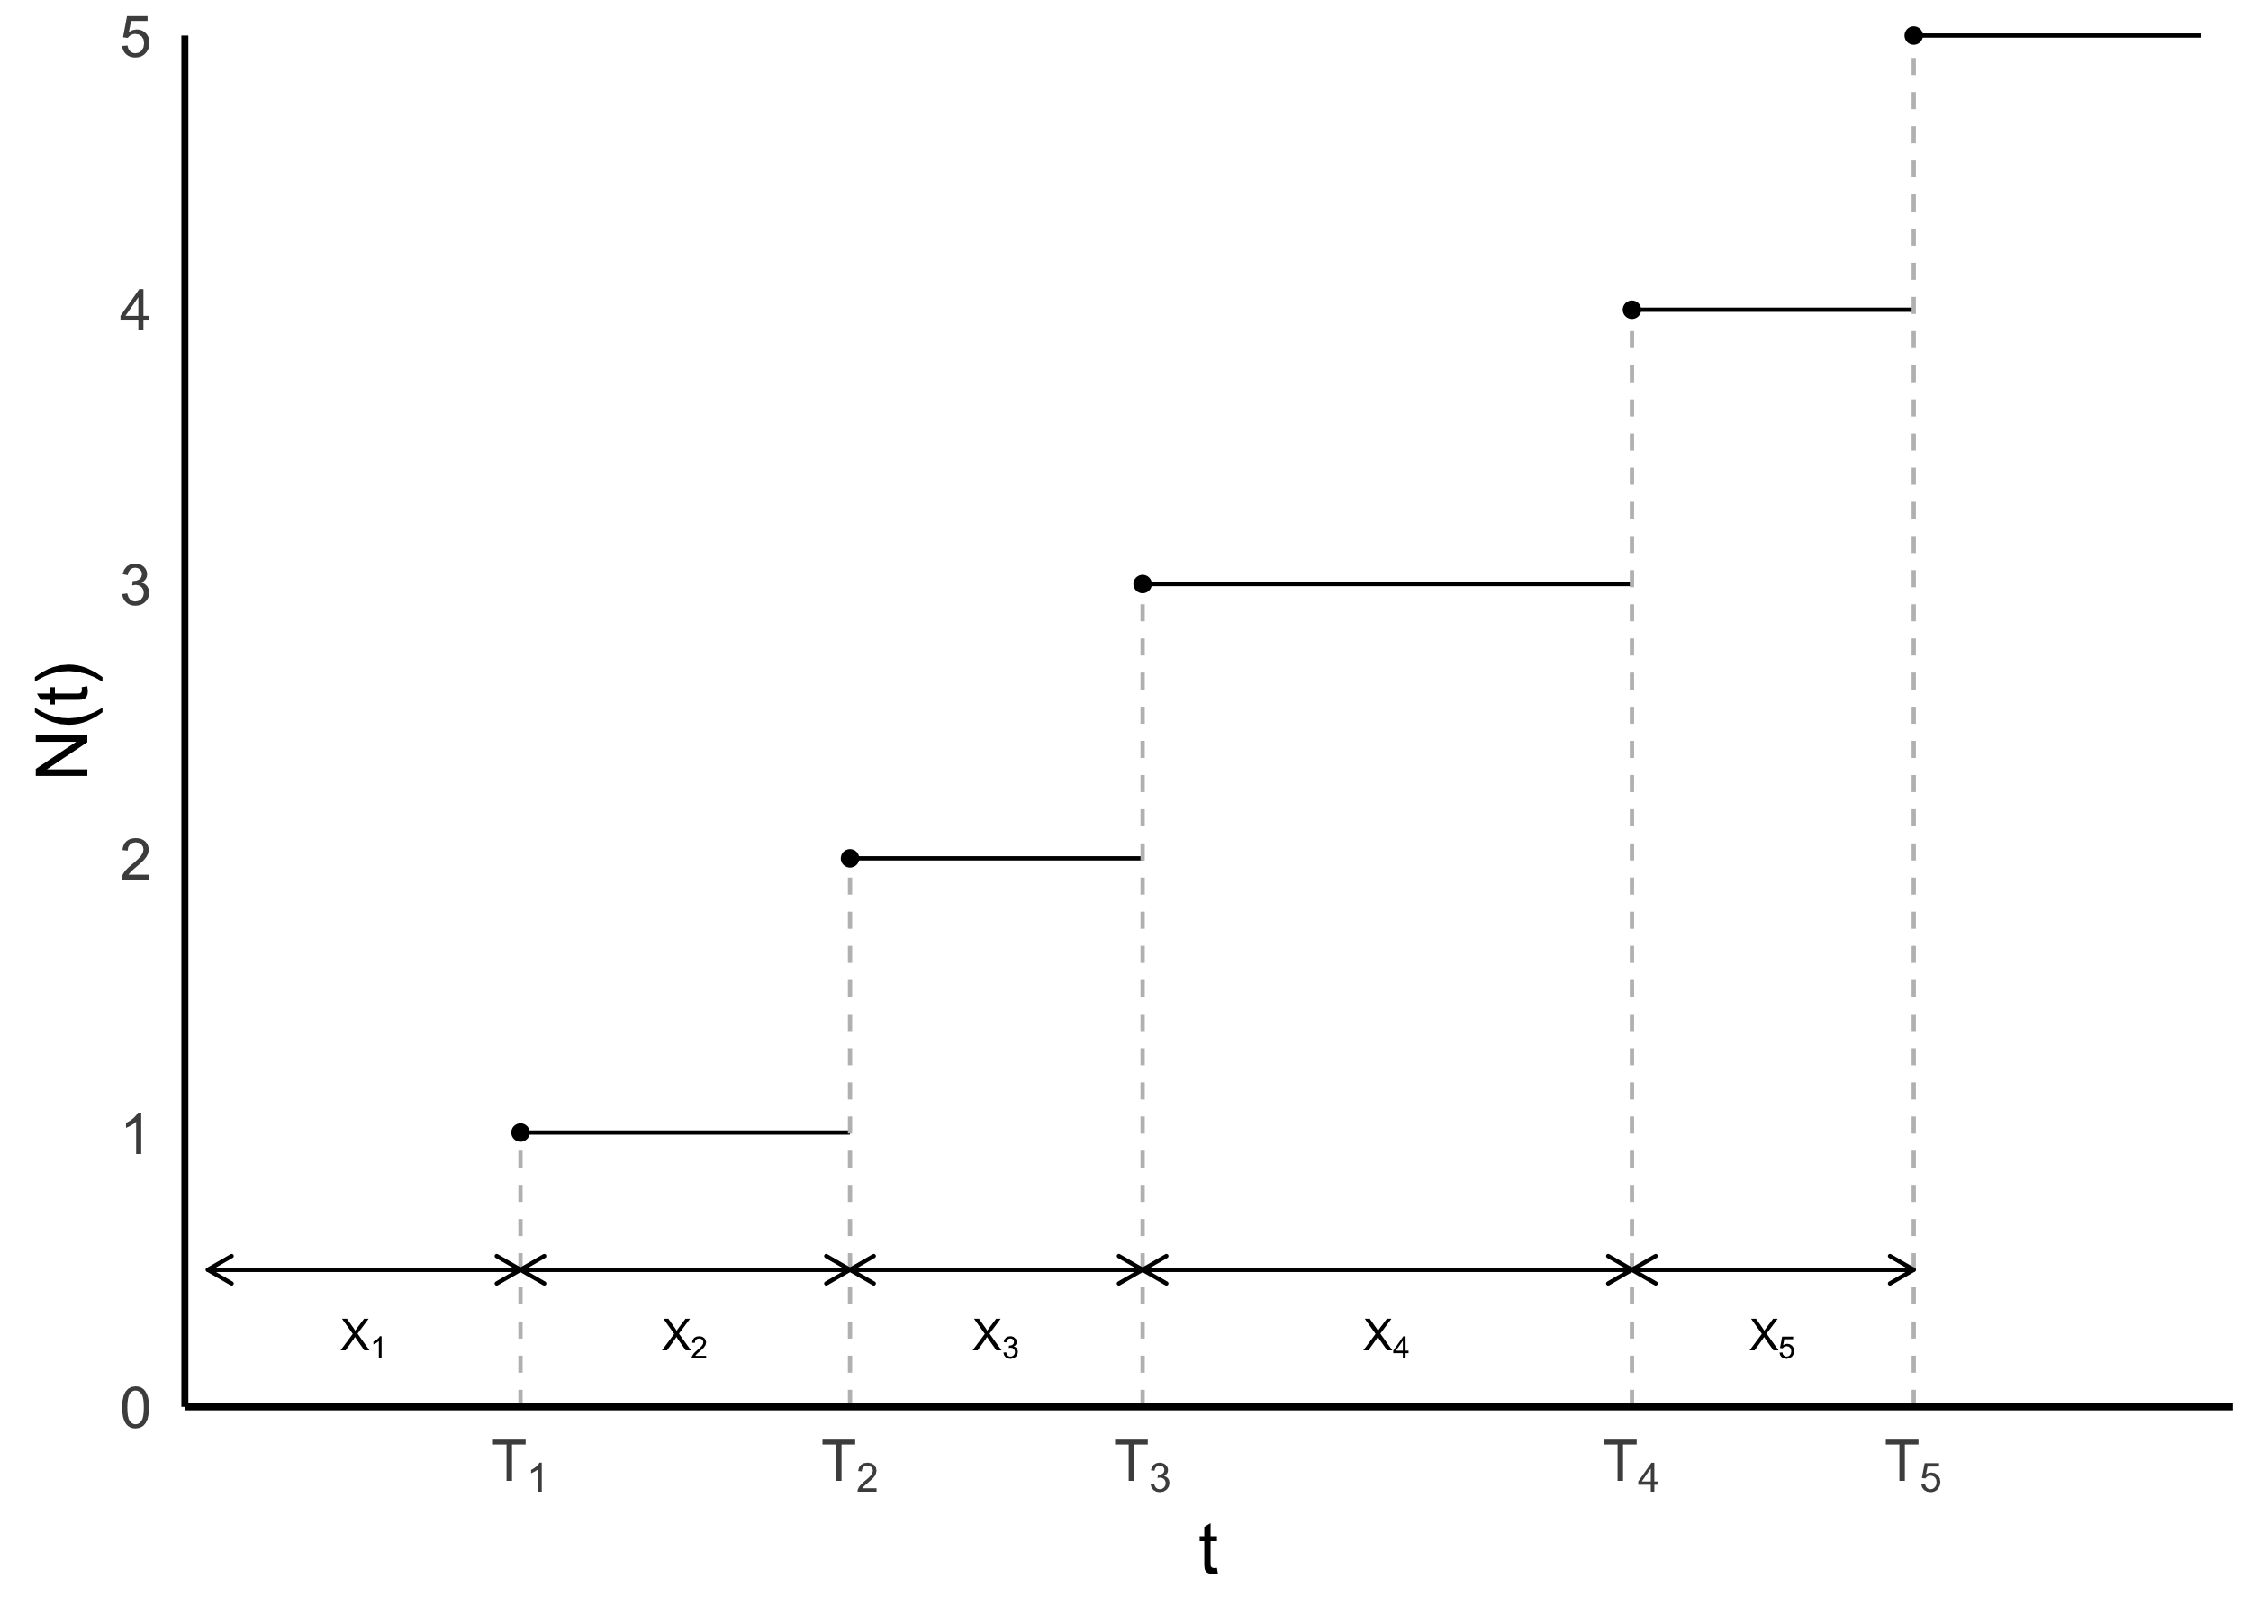
\includegraphics[width=.9\textwidth]{figures/poisson_realization.png}
   \caption{One realization of a Poisson process showing the relationship between $N(t)$, $S_n$, and $X_n$.}
  \label{fig:poisson_realization}
\end{figure}

\subsection{Matrix Exponential}

\begin{defn}[Matrix Exponential]
The matrix exponential of a real or complex $n \times n$ matrix $A$ is defined as
$$
\exp(A) = \sum_{i = 0}^\infty \frac{1}{i!} A^i
$$
where $A^0 = I$, the $n \times n$ identity matrix.
\end{defn}

\begin{theorem} \label{thm:eigen_matrix_exp}
Assume that $A$ is a diagonalizable $n \times n$ matrix with eigenvalues $\lambda_1, \lambda_2, \ldots, \lambda_n$.
Let $A = T \Lambda T^{-1}$ be the eigendecomposition of $A$ where $T$ is the $n \times n$ matrix of the eigenvectors and $\Lambda = \operatorname{diag}(\lambda_1, \ldots, \lambda_n)$.
Then,
\begin{align*}
    \exp(A) &= T \exp(\Lambda) T^{-1}\\
    &= T \operatorname{diag}(\exp(\lambda_1), \ldots, \exp(\lambda_n)) T^{-1}
\end{align*}
\end{theorem}

\section{Phase-Type distributions}

\subsection{Continuous phase-type distributions}
\begin{defn}[Phase-shift distribution] % \cite{mle_phase_type2011}
\cite{neuts1981}, \cite{maier1992}
Let $(X_t)$ be a continuous-time Markov chain with a finite state space $\Omega$ with exactly one absorbing state and $n$ transient states.
Let $Q$ be the infinitesimal generator matrix ($n + 1 \times n + 1$) for the process which has the form
$$
Q = \begin{pmatrix}
\mathbf{S} & \mathbf{S}_0\\
\mathbf{0} & 0
\end{pmatrix}
$$
Where $\mathbf{S}$ is $n \times n$, and $\mathbf{S}_0 = - \mathbf{S} \mathbf{1}$ is $n \times 1$ where $\mathbf{1}$ is a $n$ dimensional column vector of ones.
Let $\boldsymbol{\alpha}$ be a $1 \times n$ matrix of initial probabilities of starting in each state.

The distribution of the finite absorption time of the  continuous Markov chain $(X_t)$ is said to be \textbf{phase-type distributed} which we denote as $PH_c(\boldsymbol{\alpha}, S)$.
\end{defn}

\begin{theorem} \label{thm:phase-type-pdf-cdf}
Let $\tau \sim PH(\boldsymbol{\alpha}, \mathbf{S})$.
Then $\tau$ has distribution function
$$
F(x) = 1 - \boldsymbol{\alpha} \exp(x \mathbf{S}) \mathbf{1}
$$
with density
$$
f(x) = \boldsymbol{\alpha} \exp(x \mathbf{S}) \mathbf{S}_0
$$
where
$\mathbf{S}_0 = - S \mathbf{1}$.
\end{theorem}

\begin{proof}
Let $P_t$ be the transition probabilities of the process restricted to the transient states.
By the forward equations (Equation \eqref{eq:forward_eqs}), we have that $P_t' = P_t \mathbf{S}$ for $t > 0$.
The solution to the differential equation with initial condition $\boldsymbol{\alpha}$ is given by
$$
P_t = \boldsymbol{\alpha} \exp(x \mathbf{S})
$$
so
$$
F(x) = 1 - P_t \mathbf{1} = 1 - \boldsymbol{\alpha} \exp(x \mathbf{S}) \mathbf{1}
$$
It follows that
$$
f(x) = F'(x) = \boldsymbol{\alpha} \exp(x \mathbf{S}) \mathbf{S}_0
$$
\end{proof}

\begin{theorem} \label{thm:phase-moments}
Let $\tau \sim PH(\boldsymbol{\alpha}, \mathbf{S})$.
Then the moments of the distribution function are
$$
E[\tau^{{n}}]=(-1)^{{n}}n!{\boldsymbol  {\alpha }}{S}^{{-n}}{\mathbf  {1}}
$$
\end{theorem}

\begin{proof}
See \cite{neuts1981} or \cite{mle_phase_type2011}
\end{proof}

\begin{example}
The exponential distribution distribution is a phase-type distribution:
Let $\mathbf S = - \lambda$, $\mathbf{S}_0 = \lambda$ and $\boldsymbol{\alpha} = 1$.
\end{example}

\begin{example}
A mixture of 3 exponential distributions with rates $\lambda_1, \lambda_2, \lambda_3$ and weights $(\alpha_1, \alpha_2, \alpha_3)$ can be represented as a phase-type distribution:
\begin{align*}
    \mathbf S &= \begin{bmatrix}
        -\lambda_1 & 0 & 0\\
        0 & - \lambda_2 & 0\\
        0 & 0 & - \lambda_3
        \end{bmatrix}\\
    \mathbf{S}_0 &= (\lambda_1, \lambda_2, \lambda_3)^T\\
    \alpha &= (\alpha_1, \alpha_2, \alpha_3)
\end{align*}
\end{example}

\begin{defn}[Erlang Distribution] \label{defn:erlang}
A random variable $X$ is said to be Erlang distributed if it is supported on $[0, \infty)$ with two parameters: $k \in \{1,2,\ldots\}$ for the shape and $\lambda \in (0,\infty)$ for the rate with probability density function
$$
f(x) = \frac{\lambda ^{k}x^{{k-1}}e^{{-\lambda x}}}{(k-1)!}
$$
for $x, \lambda \geq 0$
\end{defn}

\begin{example}
The Erlang distribution is a phase-type distribution.
Assume we have an Erlang distribution with shape $k$ and rate $\lambda$.
The matrix $S$ will be $k \times k$ with $-\lambda$ on the diagonal and $\lambda$ on $i \times i + 1$ for all $i \in \{1, \ldots, k - 1\}$.
As an example we show that $k = 4$ has representation
\begin{align*}
    \mathbf S &= \begin{bmatrix}
        -\lambda & \lambda & 0 & 0\\
        0 & - \lambda & \lambda & 0\\
        0 & 0 & -\lambda & \lambda\\
        0 & 0 & 0 & -\lambda
        \end{bmatrix}\\
    \mathbf{S}_0 &= (0, 0, 0, \lambda)^T\\
    \alpha &= (1,0,0,0)
\end{align*}
which is easy to verify that the PDF from Theorem \ref{thm:phase-type-pdf-cdf} has the same PDF as the Erlang distribution from Definition \ref{defn:erlang}.
\end{example}

\subsection{Discrete phase-type distributions}
\begin{defn}[Discrete phase-type distribution]
\cite{neuts1981}
Let $(X_n)$ be a discrete-time Markov chain with a finite state space $\Omega$ with exactly one absorbing state and $n$ transient states.
Let $P$ be the transition probability matrix ($n + 1 \times n + 1$) for the process which has the form
$$
P = \begin{pmatrix}
\mathbf{S} & \mathbf{S}_0\\
\mathbf{0} & 0
\end{pmatrix}
$$
Where $\mathbf{S}$ is $n \times n$, and $\mathbf{S} \mathbf{1}  + \mathbf{S}_0 = \mathbf{1}$ where $\mathbf{1}$ is a $n$ dimensional column vector of ones.
Let $\boldsymbol{\alpha}$ be a $1 \times n$ matrix of initial probabilities of starting in each state.

The distribution of the first passage time to the absorbing state in the discrete-time Markov chain $(X_n)$ is denoted as $PH_d(\boldsymbol{\alpha}, S)$.

The CDF is given by
$$
F(k) = 1 - \boldsymbol{\alpha} \mathbf{S}^k \mathbf{1}
$$
with density
$$
f(k) = \boldsymbol{\alpha} \mathbf{S}^{k - 1} \mathbf{S}_0
$$
\end{defn}

\begin{example}
The geometric distribution distribution with parameter $p$ is a discrete phase-type distribution:
Let $\mathbf S = 1 - p$, $\mathbf{S}_0 = p$ and $\boldsymbol{\alpha} = 1$.
\end{example}

\begin{lemma}\cite{neuts1981}
The matrix $S$ is non-singular if and only if the states $1,\ldots, n$ of $S$ are transient.
\end{lemma}

\subsection{Closure characterisation}

\cite{neuts1975} proved the closure properties of the phase-type distributions.
That is, that the class of phase-type distributions is closed under finite mixture, finite convolutions, and geometric mixtures.
Later it was shown in \cite{maier1992}, that the phase-type distributions are the smallest class of distributions that have these properties.

\begin{defn}[Geometric Mixture] \cite{maier1992}
Let $\mu$ be a probability measure on $[0, \infty)$.
Let $N$ be a geometric random variable (supported on $\{1,2,3,\ldots\}$) with success probability $p$.
The geometric mixture, denoted $\mu^{(p)}$ is defined as
$$
\mu^{(p)} = (1 - p) [\mu + p (\mu * \mu) + p^2 (\mu * \mu * \mu) + \cdots]
$$
where $*$ denotes convolution.
\end{defn}

\begin{theorem}\cite{maier1992} Theorem 2.1

Denote $PH_c$ as the class of (continuous) phase-type distributions.

$PH_c$ is the smallest family of positive, real-valued distributions which satisfy:
\begin{enumerate}
    \item Contains all exponential distributions and the point mass at 0
    \item Closed under finite mixture and finite convolutions
    \item Closed under geometric mixtures
\end{enumerate}
\end{theorem}

\begin{theorem}\cite{maier1992} Theorem 2.2

Denote $PH_d$ as the class of discrete phase-type distributions.

$PH_d$ is the smallest family of positive, real-valued distributions which satisfy:
\begin{enumerate}
    \item Contains the point mass at 0 and point mass at 1
    \item Closed under finite mixture and finite convolutions
    \item Closed under geometric mixtures
\end{enumerate}
\end{theorem}

\begin{theorem} \cite{neuts1981}
The set of all continuous phase-type distributions is dense in the class of all positive-valued distributions.
\end{theorem}

% PH distributions are classes of distributions which can be built up from mixtures, convolutions, and the 'geometric mixture' of the point mass at 0 and all exponential distributions.

\section{Contact Process}

\begin{defn}[Contact process]
Let $S = (V,E)$ be a graph where $V$ is the set of vertices (that have bounded degree) and $E$ is the set of edges.
Let $X =  \{0,1\}^S$ be the state space.
A contact process $(\eta_t)$, is a continuous-time Markov chain on $X$ in which each 1 on the graph waits a random time, exponentially distributed, with rate 1 and then becomes a 0.
Every 0 waits exponentially with rate $k \lambda$, where $k$ is the number of edges shared with a 1.
Let $\eta$ and $\delta$ be two configurations of the graph $S$ in the process.
The transition rate matrix can be described as follow
$$
q(\eta, \delta) = \begin{cases}
    0 & \eta, \delta \text{ differ in more than one point}\\
    1 & \text{differ only at } x, \eta(x) = 1, \delta(x) = 0\\
    \lambda |\{ (x,y) \in E : \eta(y) = 1\}| & \text{differ only at } x, \eta(x) = 0, \delta(x) = 1
\end{cases}
$$

Denote $\delta_0$, $\delta_1$ be point masses on the configuration of all zeros and all ones respectively.
\end{defn}

\begin{defn}
Let $G = (V,E)$ be a graph and $X = \{0,1\}^G$ be the state space for the contact process $(\eta_t)$.
Then the extinction time of the process is denoted as
$$
\tau_{G} = \inf\{ t \geq 0 : \eta_t \equiv 0 \}
$$
\end{defn}

If the graph $S$ is finite, then the process will eventually converge to the configuration of all zeros.
When the graph $S$ is infinite, then the limiting behavior of the system varies depending on $\lambda$.
The point mass on the configuration of all zeros, $\delta_0$, is clearly a stationary distribution since no 0 is able to change to a 1.

\begin{theorem} \cite{Liggett2002}
For a contact process on d-dimensional lattice $\Z^d$ there is a critical value $\lambda_c = \lambda_c(d) \in \left( \frac{1}{2d - 1}, \frac{2}{d} \right)$ such that
\begin{itemize}
    \item If $\lambda \leq \lambda_c$ then $\eta_t$ converges weakly to $\delta_0$. % TODO: More detail on this
    \item If $\lambda > \lambda_c$ then there is some other stationary distribution $\nu \not = \delta_0$ such that $\eta_t$ converges weakly to $\nu$ for all initial configurations with infinitely many ones.
\end{itemize}
\end{theorem}

In the finite case, the system will eventually be $\equiv 0$ but \cite{Liggett1999} showed that for a finite subset $N^d$ of $Z^d$, then $\tau_{N^d}$ is logarithmic if $\lambda < \lambda_c(\Z^d)$, exponential if $\lambda > \lambda_c(\Z^d)$ and polynomial if $\lambda = \lambda_c(\Z^d)$.
Later, \cite{schapira2017}, \cite{mourrat2014phase}, and \cite{Mountford2016} showed bounds for general graphs with finite vertices.
Denote $\mathbb T^d$ as an infinite tree has exactly $d \geq 3$ edges connected to each vertex.
There are two critical values for a contact process on $\mathbb T^d$, which we denote $\lambda_c^{(1)}(\mathbb T^d)$ and $\lambda_c^{(2)}(\mathbb T^d)$.
See \cite{mourrat2014phase} for a complete description of what phase transitions occur at each of the critical values.
% TODO: Describe what happens at the two critical values?

\begin{theorem}[\cite{mourrat2014phase}]\label{thm:contact_finite_log}
For any $d \in \N$ and $\lambda < \lambda_c^{(1)}(\mathbb T^d)$ there is a constant $C > 0$ such that for any graph $G$ with at least two vertices and with bounded degree less than $d$
$$
E[\tau_{G}] \leq C \log(|G|)
$$
where $|G|$ is the number of vertices of $G$.
\end{theorem}

\begin{theorem}[\cite{Mountford2016}] \label{thm:contact_finite_exp}
For any $d \in \N$ and $\lambda > \lambda_c(\Z)$ there is a constant $k > 0$ such that for any connected graph $G$ with at least two vertices and with bounded degree less than $d$
$$
E[\tau_{G}] \geq \exp(k |G|)
$$
where $|G|$ is the number of vertices of $G$.
\end{theorem}

\begin{figure}[H]
  \centering
    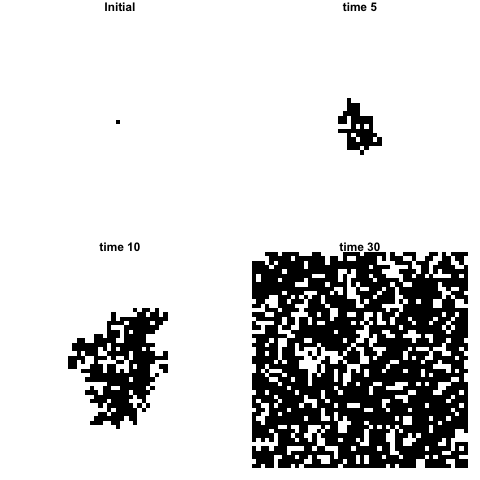
\includegraphics[width=.80\textwidth]{figures/contact_simulation_torus_25.png}
   \caption{Simulation for contact process with $\lambda = 4$ and periodic boundary conditions on $50 \times 50$ grid. The initial configuration is only one node with 1.}
  \label{fig:contact_sim_torus_above_crit.png}
\end{figure}

In Figure \ref{fig:contact_sim_torus_above_crit.png} we show one realization from a simulation of the contact process on $\{0,1\}^{(\Z/50) \times (\Z/50)}$ with $\lambda = 4 \geq \lambda_c(\Z^2)$.
This simulation follows the behavior that the time to extinction is proportional to $\exp(50 \times 50)$.
This is contrasted with Figure \ref{fig:contact_sim_torus_below_crit.png} in which $\lambda = .25$ is smaller than $\lambda_c(\Z^2)$.
The behavior seen on the graph matches shows that the extinction time is proportional to $\log(50 \times 50)$.

\begin{figure}[H]
  \centering
    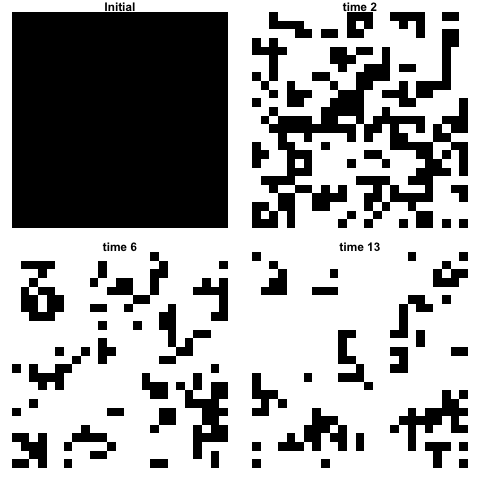
\includegraphics[width=.80\textwidth]{figures/contact_simulation_torus_25_below_crit.png}
   \caption{Simulation for contact process with $\lambda = 0.25$ on $\{0,1\}^{(\Z/50) \times (\Z/50)}$. The initial configuration has all nodes as ones.}
  \label{fig:contact_sim_torus_below_crit.png}
\end{figure}

\subsection{Contact process on finite graphs}

Now we look at a contact process on a finite graph.
We look at $\tau_{C_2}$ (which depends on $\lambda$), the time until we reach the state zero while keeping the number of nodes fixed as $\lambda$ goes to $\infty$.
% It is known that $\tau_{C_2}$ has a phase-type distribution for a fixed $\lambda$.
As $\lambda \to \infty$ then $\tau_{C_2}$ will converge to infinity in distribution so we will normalize $\tau_{C_2}$ to understand which limiting distribution one can get. This is related to the more general results in \cite{schapira2017} for the limiting distribution of the extinction time of graphs that grow in size rather than $\lambda$.

\begin{theorem}[\cite{schapira2017} Theorem 1.4]
Let $G_n$ be a graph with $n$ vertices and $(G_n)_{n \in \N}$ with $|G_n| \to \infty$ as $n \to \infty$.
Denote $\tau_{G_n}$ as the extinction time of the contact process on graph $G_n$.
For any $\lambda > \lambda_c(\Z)$
$$
\frac{\tau_{G_n}}{E[\tau_{G_n}]} \Rightarrow \exp(1)
$$
\end{theorem}

First we investigate the behavior for a complete graph, in which each node is connected to all other nodes and then we look at the one-dimensional lattice and cycles.


\subsection{Two node contact process \texorpdfstring{$C_2$}{C2}}

The contact process on the finite graph with two nodes and one edge between them has the following transition rates

\begin{align}
    1 &\to 0 \text{ at rate } 1\\
    0 &\to 1 \text{ at rate } \begin{cases}
        \lambda & \text{ if neighbor is 1}\\
        0 & \text{ otherwise}
    \end{cases}
\end{align}

We can express the infinitesimal generator matrix $Q$ matrix as

% Info on blockarray
% https://tex.stackexchange.com/a/59519/41827
$$
Q = \begin{blockarray}{ccccc}
    & (1,1) & (1,0) & (0,1) & (0,0)\\
    \begin{block}{c(cccc)}
        (1,1) & -2 & 1 & 1 & 0\\
        (1,0) & \lambda & - 1 - \lambda & 0 & 1\\
        (0,1) & \lambda & 0 & - 1 - \lambda & 1\\
        (0,0) & 0 & 0 & 0 & 0\\
    \end{block}
\end{blockarray}
$$
Start the process with both nodes at 1.
We can project this continuous-time Markov chain to the number of ones in the process at a given time.
Map $(1,1)$ to 2, $\{(1,0),(0,1)\}$ to a single state 1, and $(0,0)$ to 0.
This new chain is also a Markov chain by Theorem \ref{thm:mc_projection}.

\begin{equation}\label{eq:q_c_2}
Q_{C_2} = \begin{blockarray}{cccc}
    & 2 & 1 & 0\\
    \begin{block}{c(ccc)}
        2 & -2 & 2 & 0\\
        1 & \lambda & - (1 + \lambda) & 1\\
        0 & 0 & 0 & 0\\
    \end{block}
\end{blockarray}
\end{equation}


\begin{figure}[H]
    \centering
   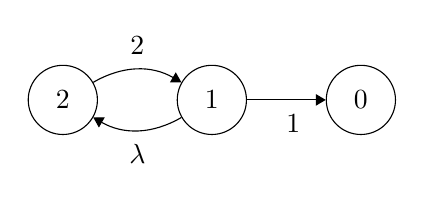
\begin{tikzpicture}[start chain = going right,
   -Triangle, every loop/.append style = {-Triangle}]
   \node[state, on chain]  (2) {2};
   \node[state, on chain]  (1) {1};
   \node[state, on chain]  (0) {0};

   \draw (2) edge[bend left] node[yshift=3mm]{$2$} (1);
   \draw (1) edge[bend left] node[yshift=-3mm]{$\lambda$}(2);
   \draw (1) edge[left] node[xshift=3mm, yshift=-3mm]{$1$} (0);

\end{tikzpicture}
    \caption{Rates for two node projected contact process}
    \label{fig:rates_mc_two_contact}
\end{figure}

\begin{figure}[H]
    \centering
   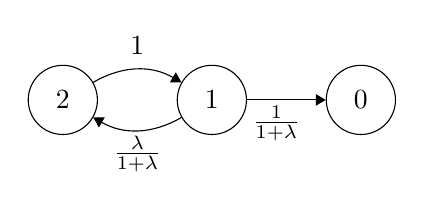
\begin{tikzpicture}[start chain = going right,
   -Triangle, every loop/.append style = {-Triangle}]
   \node[state, on chain]  (2) {2};
   \node[state, on chain]  (1) {1};
   \node[state, on chain]  (0) {0};

   \draw (2) edge[bend left] node[yshift=3mm]{$1$} (1);
   \draw (1) edge[bend left] node[yshift=-3mm]{$\frac{\lambda}{1 + \lambda}$}(2);
   \draw (1) edge[left] node[xshift=3mm, yshift=-3mm]{$\frac{1}{1 + \lambda}$} (0);

\end{tikzpicture}
    \caption{Embedded Markov chain for two node projected contact process}
    \label{fig:discrete_mc_two_contact}
\end{figure}

Let $\tau_{C_2}$ be the time in which we hit 0.
The waiting time while in state 2 is exponentially distributed random variable $X$ with parameter $- q_{2} = 2$ and similarly the waiting time while in state 1 is exponentially distributed with parameter $- q_{(1,0)} = 1 + \lambda$.

The embedded Markov chain for the process is the discrete-time Markov chain of the jumps in the process.
For example if the original process $(A_t)$ is $A_{0} = 2, A_{.75} = 1, A_{1.2} = 2, \ldots, A_{23.2} = 0$ then the embedded chain $(B_n)$ is $B_{0} = 2, B_1 = 1, B_2 = 2, \ldots, B_n = 0$.
The probability of going from one state to another is shown in Figure \ref{fig:discrete_mc_two_contact}.

Let $N$ be a geometric random variable which denotes the number of times that the process waits at state 1 before moving to the absorbing state 0.
It has a success parameter $\frac{1}{1 + \lambda}$ which represents going to the absorbing state 0.
Also, let $X_1, X_2, \ldots$ be i.i.d random variables with
$X_i \sim \exp(2)$ for the waiting time at state 2 and independent of i.i.d random variables $Y_1, Y_2, \ldots$ with  $Y_i \sim \exp(1 + \lambda)$ for the waiting time at state 1.
The random variable $N$ is independent of both $(X_n)$ and $(Y_n)$ from Theorem \ref{thm:x_N_indep}.

Now we can express $\tau_{C_2}$ as a random sum
$$
\tau_{C_2} = \sum_{i = 1}^N (X_i + Y_i)
$$

\begin{theorem}
$$
E[\tau_{C_2}] = \frac{3}{2} + \frac{\lambda}{2}
$$
and
$$
\Var(\tau_{C_2}) = \frac{\lambda^2 + 6 \lambda + 5}{4}
$$
\end{theorem}

\begin{proof}
$$
P(N = n) = \left(\frac{\lambda}{1 + \lambda} \right)^{n - 1} \frac{1}{1 + \lambda} \quad n = 1,2,\ldots
$$
with
\begin{align*}
    E[N] &= 1 + \lambda\\
    \Var(N) &= \frac{\lambda/(1 + \lambda)}{1/(1 + \lambda)^2} = \lambda (1 + \lambda)
\end{align*}
Also since $(X_n)$ and $(Y_n)$ are independent,

\begin{align*}
    E[X_i + Y_i] &= E[X + Y] = \frac{3 + \lambda}{2(1 + \lambda)}\\
    \Var(X_i + Y_i) &= \Var(X + Y) = \frac{(1 + \lambda)^2 + 4}{4(1 + \lambda)^2}
\end{align*}

Since both $(X_n)$ and $(Y_n)$ are mutually independent of $N$ then by Theorem \eqref{thm:random_sum_ev},
$$
E[\tau_{C_2}] = E\left[ \sum_{i = 1}^N X_i + Y_i \right] = E[X + Y] E[N] = \frac{3 + \lambda}{2(1 + \lambda)} \cdot (1 + \lambda) = \frac{3}{2} + \frac{\lambda}{2}
$$

By Theorem \ref{thm:random_sum_var}
\begin{align*}
    \Var\left( \sum_{i = 1}^N X_i + Y_i \right) &= E[N]\Var(X + Y) + (E[X + Y])^2 \Var(N)\\
    &= (1 + \lambda) \frac{(1 + \lambda)^2 + 4}{4(1 + \lambda)^2} + \frac{(3 + \lambda)^2}{4 (1 + \lambda)^2} \lambda (1 + \lambda)\\
    &= \frac{
        (1 + \lambda)^2 + 4 + (3 + \lambda)^2 \lambda
    }{4(1 + \lambda)}\\
    &= \frac{
    \lambda^3 + 7 \lambda^2 + 11 \lambda + 5
    }{4(1 + \lambda}\\
    &= \frac{\lambda^2 + 6 \lambda + 5}{4}
\end{align*}
\end{proof}

\subsubsection{Phase-type distribution}

The time to absorption $\tau_{C_2}$ has a phase-type distribution.
We can decompose $Q_{C_2}$, Equation \eqref{eq:q_c_2}, as
% $$
% Q_{C_2} = \begin{blockarray}{cccc}
%     & 2 & 1 & 0\\
%     \cline{2-4}
%     \begin{block}{c|cc|c|}
%         2 & -2 & 2 & 0\\
%         1 & \lambda & - (1 + \lambda) & 1\\
%         \cline{2-3}
%     \end{block}
%     \begin{block}{c|ccc|}
%         0 & 0 & 0 & 0\\
%     \end{block}
% \end{blockarray}
% $$
\begin{align*}
    \mathbf{S} &= \begin{pmatrix}
        -2 & 2\\
        \lambda & - (1 + \lambda)
    \end{pmatrix}\\
    \mathbf{S}_0 &= \begin{pmatrix}
        0\\
        1
    \end{pmatrix}\\
    \boldsymbol{\alpha} &= \begin{pmatrix}
    1 & 0
    \end{pmatrix}
\end{align*}

To compute the matrix exponential $\exp(x S)$ we first compute the eigenvalues of $S$.
Solving $\det(S - m I) = 0$ for $m$,
\begin{align*}
    \det(S - m I) &= \det\left(\begin{bmatrix}
        -2 - m & 2\\
        \lambda & - 1 - \lambda - m
    \end{bmatrix} \right)\\
    &= (2 + m) (1 + \lambda + m) - 2 \lambda\\
    &= 2 + (3 + \lambda) m + m^2
\end{align*}
Solving the equation $2 + (3 + \lambda) m + m^2 = 0$ for $m$ we get roots (eigenvalues)
\begin{align*}
    m_1 &= \frac{1}{2}(-3 - \lambda + \sqrt{\lambda^2 + 6 \lambda + 1})\\
    m_2 &= \frac{1}{2}(-3 - \lambda - \sqrt{\lambda^2 + 6 \lambda + 1})
\end{align*}
So $\lambda_1 = x m_1$, $\lambda_2 = x m_2$ are the eigenvalues for $x S$.
Denote
$$
\Lambda = \operatorname{diag}(\lambda_1, \lambda_2)
$$
and
$$
C = \sqrt{\lambda^2 + 6 \lambda + 1}
$$
Then solving $(S - m I) \mathbf{v} = 0$ for $m_1, m_2$, we get eigenvectors
\begin{align*}
    v_1 &= \left( \frac{-1 + \lambda - C}{2\lambda}, 1 \right)\\
    v_2 &= \left( \frac{-1 + \lambda + C}{2\lambda}, 1 \right)
\end{align*}
Let
$$
U = \begin{bmatrix}
    \frac{-1 + \lambda - C}{2\lambda} & \frac{-1 + \lambda + C}{2\lambda}\\
    1 & 1
\end{bmatrix}
$$
hence
$$
\det(U) = - \frac{C}{\lambda}
$$
It follows that
\begin{align*}
    U^{-1} &= - \frac{\lambda}{C} \begin{bmatrix}
    1 & \frac{1 - \lambda - C}{2\lambda}\\
    -1 & \frac{-1 + \lambda - C}{2\lambda}
    \end{bmatrix}\\
    &= \frac{1}{2C} \begin{bmatrix}
    -2\lambda & -1 + \lambda + C\\
    2\lambda & 1 - \lambda + C
    \end{bmatrix}
\end{align*}

% Now by Theorem \ref{thm:eigen_matrix_exp}, we can compute $\exp(xS)$ as
% \begin{align*}
% \exp(xS) &= T \begin{bmatrix}
%     \exp(\frac{1}{2}(-3 - \lambda + C)) & 0\\
%     0 & \exp(\frac{1}{2}(-3 - \lambda - C))
% \end{bmatrix} T^{-1}\\
% &= - \frac{1}{2 C} T \begin{bmatrix}
%     \exp(\frac{-3 - \lambda + C}{2}) & \exp(\frac{-3 - \lambda + C}{2}) \frac{1 - \lambda - C}{2\lambda} \\
%     - \exp(\frac{-3 - \lambda - C}{2}) & \exp(\frac{1}{2}(-3 - \lambda - C)) \frac{-1 + \lambda - C}{2\lambda}
% \end{bmatrix}
% \end{align*}

The density of $\tau_{C_2}$ is defined as
\begin{align*}
 f(x; \lambda) &= \boldsymbol{\alpha} \exp(x \mathbf{S}) \mathbf{S}_0 \nonumber\\
 &= (1, 0) \exp(\mathbf{S} x) (0,1)^T \\
 &= (1, 0) U \exp(\Lambda) U^{-1} (0,1)^T
\end{align*}
Where
\begin{align*}
    (1,0) U &= (1,0) \begin{bmatrix}
    \frac{-1 + \lambda - C}{2\lambda} & \frac{-1 + \lambda + C}{2\lambda}\\
    1 & 1
\end{bmatrix}\\
    &= \begin{bmatrix}
    \frac{-1 + \lambda - C}{2\lambda} & \frac{-1 + \lambda + C}{2\lambda}
    \end{bmatrix}
\end{align*}
and
\begin{align*}
    U^{-1} (0,1)^T &= \frac{1}{2C} \begin{bmatrix}
    -2\lambda & -1 + \lambda + C\\
    2\lambda & 1 - \lambda + C
    \end{bmatrix} (0,1)^T\\
    &= \frac{1}{2C} \begin{bmatrix}
    -1 + \lambda + C\\
    1 - \lambda + C
    \end{bmatrix}
\end{align*}

Thus
\begin{align*}
     f(x; \lambda) &= (1, 0) U \exp(\Lambda) U^{-1} (0,1)^T\\
     &= \frac{1}{2C} \begin{bmatrix}
    \frac{-1 + \lambda - C}{2\lambda} & \frac{-1 + \lambda + C}{2\lambda}
    \end{bmatrix} \exp(\Lambda)  \begin{bmatrix}
    -1 + \lambda + C\\
    1 - \lambda + C
    \end{bmatrix}\\
    &= \frac{1}{2C} \left( 4 \exp\left(\frac{1}{2}(-3 - \lambda + C) x\right) - 4 \exp\left(\frac{1}{2}(-3 - \lambda - C) x\right) \right)\\
    &= \frac{2}{C} \left( \exp\left(\frac{1}{2}(-3 - \lambda + C) x\right) - \exp\left(\frac{1}{2}(-3 - \lambda - C) x\right) \right)\\
\end{align*}
Note that the left exponential and right exponential differ only by sign on the term $C$.
Finally plugging back in $C$ we get
\begin{equation} \label{eq:t_density}
      f(x; \lambda) = \frac{2 \exp\left(\frac{1}{2}(-3 - \lambda + \sqrt{\lambda^2 + 6 \lambda + 1}) x\right)}{\sqrt{\lambda^2 + 6 \lambda + 1}}  - \frac{2 \exp\left(\frac{1}{2}(-3 - \lambda - \sqrt{\lambda^2 + 6 \lambda + 1}) x\right)}{\sqrt{\lambda^2 + 6 \lambda + 1}}
\end{equation}

% \begin{align}
% f(x; \lambda) &= \boldsymbol{\alpha} \exp(x \mathbf{S}) \mathbf{S}_0 \nonumber\\
% &= (1, 0) \exp(\mathbf{S} x) (0,1)^T \nonumber\\
% &= (1, 0) T \begin{bmatrix}
%     \exp(\frac{1}{2}(-3 - \lambda + \sqrt{\lambda^2 + 6 \lambda + 1})) & 0\\
%     0 & \exp(\frac{1}{2}(-3 - \lambda - \sqrt{\lambda^2 + 6 \lambda + 1}))
% \end{bmatrix} T^{-1}
% (0,1)^T \nonumber\\
% &=
% \left(\frac{-1 + \lambda - \sqrt{\lambda^2 + 6 \lambda + 1}}{2\lambda}, 1\right) \nonumber \\
% &\quad\quad \begin{bmatrix}
%     \exp(\frac{1}{2}(-3 - \lambda + \sqrt{\lambda^2 + 6 \lambda + 1})) & 0\\
%     0 & \exp(\frac{1}{2}(-3 - \lambda - \sqrt{\lambda^2 + 6 \lambda + 1}))
% \end{bmatrix} \nonumber\\
% &\quad\quad  \begin{bmatrix}
%     \frac{1 - \lambda - \sqrt{\lambda^2 + 6 \lambda + 1}}{2\lambda}\\
%     \frac{-1 + \lambda - \sqrt{\lambda^2 + 6 \lambda + 1}}{2\lambda}
% \end{bmatrix} \nonumber
% \end{align}

% MatrixExp[{{-2 x, 2 x}, {\[Lambda] x, -((1 + \[Lambda]) x)}}] // TeXForm

% Using Wolfram Language we can compute the matrix exponential which is complicated even in this simple case. Let $A = \exp(Sx)$.

% \begin{align*}
% A_{11} &= \frac{\left(C+\lambda -1\right) e^{\frac{1}{2}
%   \left(C-\lambda -3\right) x}}{2 C}\\
%   &\quad\quad- \frac{\left(-C+\lambda -1\right)
%   e^{\frac{1}{2} \left(-C-\lambda -3\right) x}}{2
%   C}\\
%   A_{12} &= \frac{2 e^{\frac{1}{2} \left(C-\lambda -3\right) x}}{C}-\frac{2
%   e^{\frac{1}{2} \left(-C-\lambda -3\right)
%   x}}{C}\\
%   A_{21} &= \frac{\lambda  e^{\frac{1}{2} \left(C-\lambda -3\right)
%   x}}{C}-\frac{\lambda  e^{\frac{1}{2}
%   \left(-C-\lambda -3\right) x}}{C}\\
%   A_{22} &= \frac{\left(C-\lambda +1\right)
%   e^{\frac{1}{2} \left(C-\lambda -3\right) x}}{2
%   C}\\
%   &\quad\quad-\frac{\left(-C-\lambda +1\right) e^{\frac{1}{2} \left(-C-\lambda
%   -3\right) x}}{2 C}
% \end{align*}

% Then the density of $\tau_{C_2}$ is defined as
% \begin{align}
% f(x; \lambda) &= \boldsymbol{\alpha} \exp(x \mathbf{S}) \mathbf{S}_0 \nonumber\\
% &= (1, 0) \exp(\mathbf{S} x) (0,1)^T \nonumber\\
% &= \exp(\mathbf{S} x)_{12} \nonumber\\
% &= \frac{2 e^{\frac{1}{2} \left(\sqrt{\lambda ^2+6
%   \lambda +1}-\lambda -3\right) x}}{C}-\frac{2
%   e^{\frac{1}{2} \left(-C-\lambda -3\right)
%   x}}{C} \label{eq:t_density}
% \end{align}

\begin{figure}[H]
  \centering
    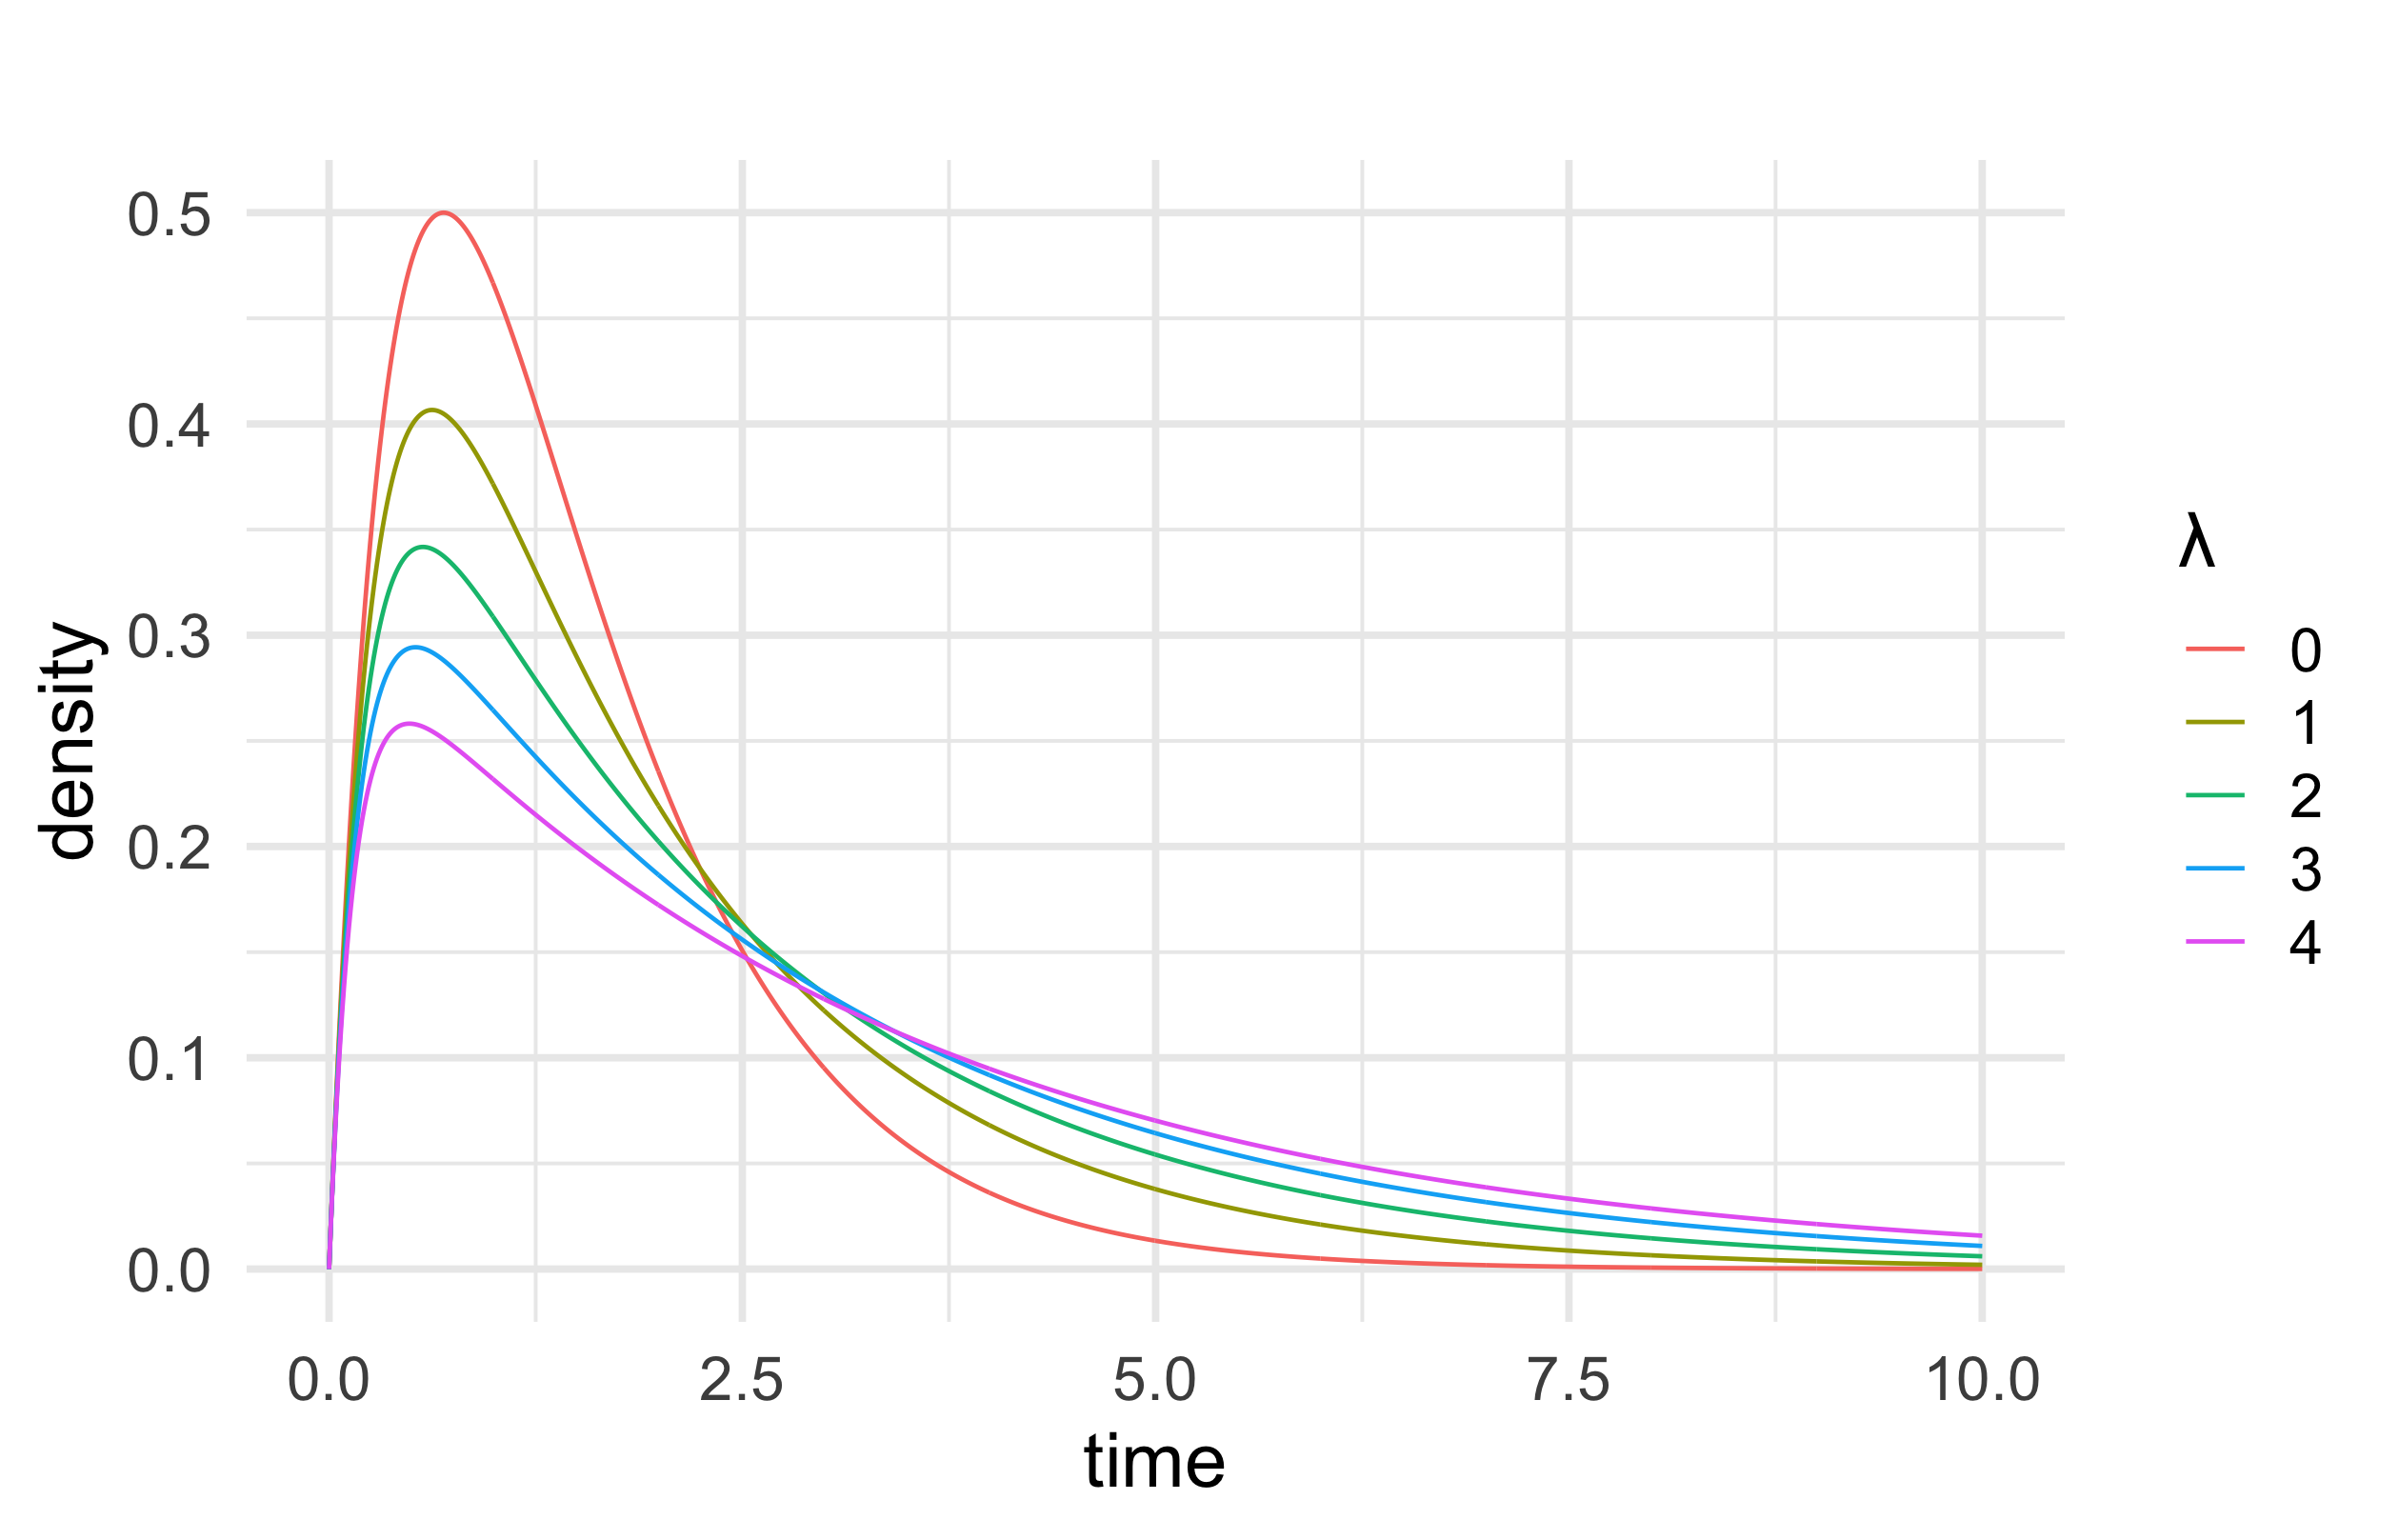
\includegraphics[width=.80\textwidth]{figures/complete_2_contact_phase_densities.png}
   \caption{Density functions for $\tau_{C_2}$ for $\lambda = 1, 2, 3, 4$ on the contact process with two nodes}
  \label{fig:contact_2_phase_densities}
\end{figure}

In Figure \ref{fig:contact_2_phase_densities} we plot the density from Equation \ref{eq:t_density} for $\lambda = 1, 2, 3, 4$.
It is clear that as $\lambda \to \infty$ then $\tau_{C_2}$ approaches infinity in distribution.
For all of the more complex models we will use numerical methods for approximating the phase-type distribution rather than the symbolic algebra method.
We sample and simulate from the phase-type distributions using the R package from \cite{actuar2008}.

\subsubsection{Limiting Distribution}

\begin{theorem}
Let $\tau_{C_2}$ be the time in which we hit $(0,0)$.
Then $\frac{2}{1 + \lambda} \tau_{C_2}$ approaches an exponential distribution with rate 1 in distribution as $\lambda \to \infty$.
\end{theorem}

\begin{proof}
Let $X_1, X_2, \ldots$ be i.i.d random variables with
$X_i \sim \exp(2)$ and independent of i.i.d random variables $Y_1, Y_2, \ldots$ with  $Y_i \sim \exp(1 + \lambda)$ and
$N$ geometrically distributed (supported on $\{1,2,\ldots\}$) with parameter $\frac{1}{1 + \lambda}$, independent of $(X_n)$ and $(Y_n)$.

$\tau_{C_2}$ is expressed as a random sum
$$
\tau_{C_2} = \sum_{i = 1}^N (X_i + Y_i)
$$

By Theorem \ref{thm:geom_sum_exp}, we have that
\begin{align*}
    \sum_{i = 1}^N X_i &\sim \exp\left( \frac{2}{1 + \lambda} \right)\\
    \sum_{i = 1}^N Y_i &\sim \exp( 1 )
\end{align*}

Using the scaling property of exponential random variables (Theorem \ref{thm:exp_scaling}) we have that
\begin{align*}
    \frac{2}{1 + \lambda}\sum_{i = 1}^N X_i &\sim \exp( 1 )\\
    \frac{2}{1 + \lambda}\sum_{i = 1}^N Y_i &\sim \exp \left( \frac{1 + \lambda}{2} \right)
\end{align*}

Let $W_\lambda \sim \exp \left( \frac{1 + \lambda}{2} \right)$ with $F_\lambda$ the distribution function, that is $F_\lambda(x) = 1 - \exp(-(1 + \lambda)/2 x)$.
As $\lambda \to \infty$, then $F_\lambda(x) \to 1$ for $x \in [x, \infty)$, so $W_n \Rightarrow 0$.
Then by Theorem \ref{thm:conv_together_lemma}, we have that $\frac{2}{1 + \lambda} \tau_{C_2} \Rightarrow \exp(1)$.
\end{proof}

\subsection{Three node contact process \texorpdfstring{$C_3$}{C3}}
Now we look at the three node contact process on a complete graph.
Again we project the states to the number of ones in the process which will be a Markov chain by Theorem \ref{thm:mc_projection}, as shown in Figure \ref{fig:mc_three_contact}.

% {{-3x, 3x, 0}, {2\[Lambda] x, -(2 + 2 \[Lambda]) x, 2x}, {0, 2\[Lambda]x, -(1 + 2\[Lambda])x}}
% Computing the matrix exponential is crazy. Better to leave numeric.
\begin{equation}
Q_{C_3} = \begin{blockarray}{ccccc}
    & 3 & 2 & 1 & 0\\
    \begin{block}{c|cccc}
    \cline{2-5}
        3 & -3 & 3 & 0 & 0 \\
        2 & 2\lambda & -(2 + 2 \lambda) &
        2 & 0\\
        1 & 0 & 2\lambda & -(1 + 2\lambda) & 1\\
    0 & 0 & 0 & 0 & 0\\
    \end{block}
\end{blockarray}
\end{equation}

Now let $N_1, N_2, N_3$ be the number of visits to states 1, 2, and 3, respectively.
Let $X_i^{(1)} \sim \exp(1 + 2\lambda)$ be i.i.d random variables, $X_i^{(2)} \sim \exp(2 + 2\lambda)$ i.i.d and $X_i^{(3)} \sim \exp(3)$ i.i.d.
Note that $N_1, N_2, N_3$ are not independent of each other, but for each $i$ each state is independent of the waiting times at the state.
We can again represent $\tau_{C_3}$ as a random sum

\begin{figure}[H]
    \centering
   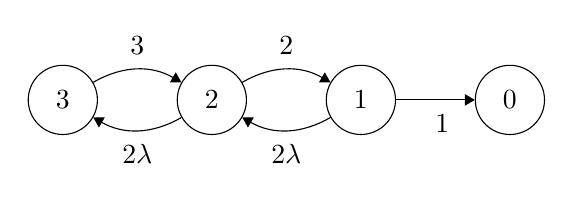
\begin{tikzpicture}[start chain = going right,
   -Triangle, every loop/.append style = {-Triangle}]
   \node[state, on chain]  (3) {3};
   \node[state, on chain]  (2) {2};
   \node[state, on chain]  (1) {1};
   \node[state, on chain]  (0) {0};

   \draw (3) edge[bend left] node[yshift=3mm]{$3$} (2);
   \draw (2) edge[bend left] node[yshift=-3mm]{$2\lambda$}(3);
   %
   \draw (2) edge[bend left] node[yshift=3mm]{$2$} (1);
   \draw (1) edge[bend left] node[yshift=-3mm]{$2\lambda$}(2);
   %
   \draw (1) edge[left] node[xshift=3mm, yshift=-3mm]{$1$} (0);

\end{tikzpicture}
    \caption{Projected Markov chain rates of number of ones for three node contact process}
    \label{fig:mc_three_contact}
\end{figure}

\begin{equation}
    \tau_{C_3} = \sum_{i = 1}^{N_3} X_i^{(3)} + \sum_{i = 1}^{N_2} X_i^{(2)} + \sum_{i = 1}^{N_1} X_i^{(1)}
\end{equation}

Then the discrete time Markov chain for this process can be expressed in canonical form as
$$
P_{C_3} = \begin{blockarray}{ccccc}
    & 3 & 2 & 1 & 0\\
    \begin{block}{c|ccc|c}
    \cline{2-5}
        3 & 0 & 1 & 0 & 0 \\
        2 & \frac{\lambda}{1 + \lambda} & 0 &
        \frac{1}{1 + \lambda} & 0\\
        1 & 0 & \frac{2\lambda}{1 + 2 \lambda} & 0 & \frac{1}{1 + 2\lambda}\\
    \cline{2-4}
    \end{block}
    \begin{block}{c|cccc}
    0 & 0 & 0 & 0 & 1\\
    \end{block}
\end{blockarray}
$$

\begin{figure}[H]
    \centering
   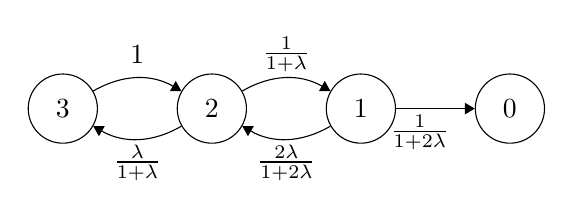
\begin{tikzpicture}[start chain = going right,
   -Triangle, every loop/.append style = {-Triangle}]
   \node[state, on chain]  (3) {3};
   \node[state, on chain]  (2) {2};
   \node[state, on chain]  (1) {1};
   \node[state, on chain]  (0) {0};

   \draw (3) edge[bend left] node[yshift=3mm]{$1$} (2);
   \draw (2) edge[bend left] node[yshift=-3mm]{$\frac{ \lambda}{1 + \lambda}$}(3);
   %
   \draw (2) edge[bend left] node[yshift=3mm]{$\frac{1}{1 + \lambda}$} (1);
   \draw (1) edge[bend left] node[yshift=-3mm]{$\frac{2\lambda}{1 + 2 \lambda}$}(2);
   %
   \draw (1) edge[left] node[xshift=3mm, yshift=-3mm]{$\frac{1}{1 + 2\lambda}$} (0);

\end{tikzpicture}
    \caption{Embedded discrete Markov chain for projection to number of ones for three node contact process}
    \label{fig:discrete_mc_three_contact}
\end{figure}

Since the discrete Markov chain is absorbing, with 0 as an absorbing state, we can compute the expected number of visits to each state using the fundamental matrix.

% Wolfram:
% B = {{1, -1, 0},{-x/(2 + x), 1, -2/(2 + x)},{0, -2x/(1 + 2x), 1}}
% inverse of {{1, -1, 0},{-x/(1 + x), 1, -1/(1 + x)},{0, -2x/(1 + 2x), 1}}

Let $B$ be the transition matrix for the transient states 3, 2, and 1.
$$
B_{C_3} = \begin{blockarray}{cccc}
    & 3 & 2 & 1\\
    \begin{block}{c|ccc}
    \cline{2-4}
        3 & 0 & 1 & 0\\
        2 & \frac{\lambda}{1 + \lambda} & 0 &
        \frac{1}{1 + \lambda}\\
        1 & 0 & \frac{2\lambda}{1 + 2 \lambda} & 0\\
    \end{block}
    \end{blockarray}
$$
Then by Theorem \ref{thm:fund_exp} the expected number of times that the contact process has a given state is given by,
$$
    I + B_{C_3} + B_{C_3}^2 + \cdots = (I - B_{C_3})^{-1} = \begin{blockarray}{cccc}
    & 3 & 2 & 1\\
    \begin{block}{c|ccc}
    \cline{2-4}
    3 & 2 \lambda^2 + \lambda + 1 & (\lambda + 1) (2 \lambda + 1) &  2 \lambda + 1\\
    2 & \lambda (2 \lambda + 1) & (\lambda + 1)(2 \lambda + 1) & 2 \lambda + 1\\
    1 & 2 \lambda^2 & 2 \lambda ( \lambda + 1) &  2\lambda + 1\\
    \end{block}
    \end{blockarray}
$$
The first row corresponds to the expected number of visits to each state given that we started in state 3 (all the nodes initialized to 1).
Thus,
\begin{align*}
    E[N_1] &= 2 \lambda + 1\\
    E[N_2] &= (\lambda + 1) (2 \lambda + 1) = 2\lambda^2 + 3 \lambda + 1\\
    E[N_3] &=  2 \lambda^2 + \lambda + 1
\end{align*}

Since $N_1, N_2, N_3$ are all geometrically distributed and are completely determined by the mean we can conclude that
\begin{align*}
    N_1 &\sim  \text{Geom}\left(\frac{1}{2 \lambda + 1} \right)\\
    N_2 &\sim \text{Geom}\left(\frac{1}{2\lambda^2 + 3 \lambda + 1} \right)\\
    N_3 &\sim  \text{Geom}\left(\frac{1}{2 \lambda^2 + \lambda + 1}\right)
\end{align*}

It then follow that
\begin{align*}
        E[\tau_{C_3}] &= E[N_3] E[X_i^{(3)}] + E[N_2] E[X_i^{(2)}] + E[N_1] E[X_i^{(1)}]\\
        &= \frac{\lambda^2 + \lambda + 1}{3} + \frac{(\lambda + 1)(2 \lambda + 1)}{2 (\lambda + 1)} + \frac{1 + 2\lambda}{1 + 2 \lambda}\\
        &= \frac{1}{6}(4 \lambda^2 + 8 \lambda + 11)
\end{align*}

\subsubsection{Phase-type Distribution}

The exact distribution of $\tau_{C_3}$ for a fixed $\lambda$ is computed numerically.
We plot the density functions for $\tau_{C_3}$ for $\lambda = 1, 2, 3, 4$ on the complete three node contact process.

\begin{figure}[H]
  \centering
    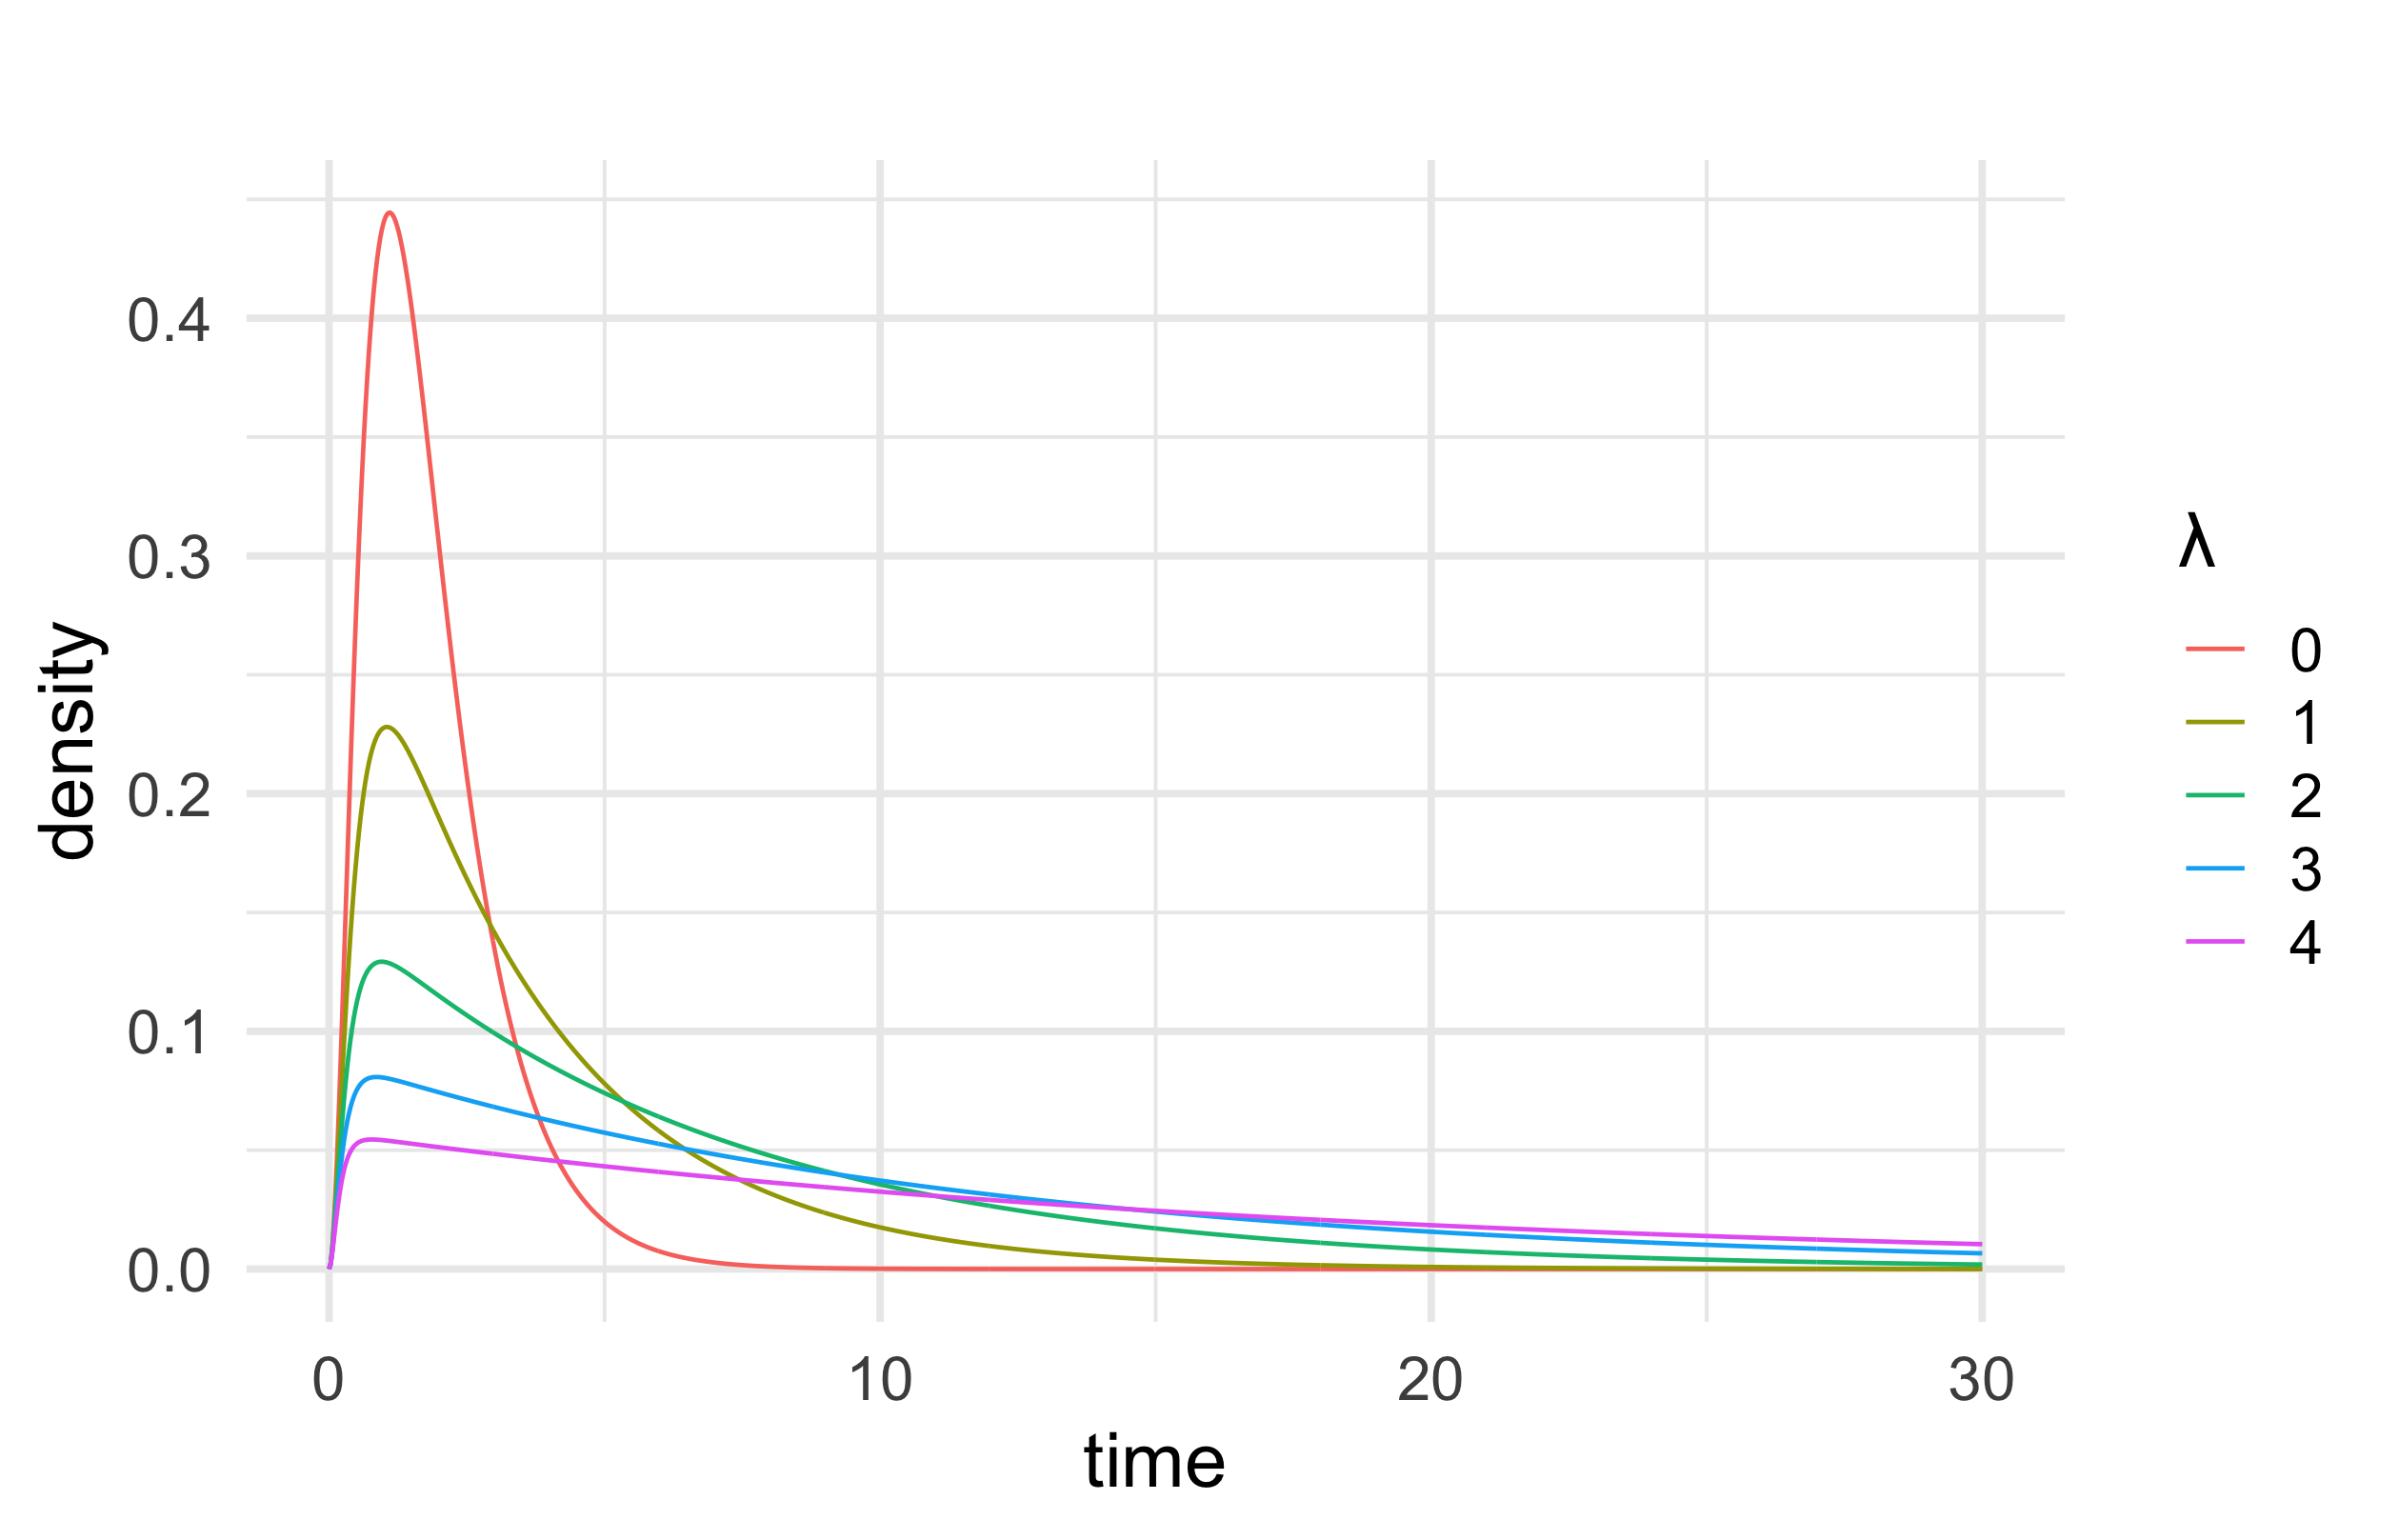
\includegraphics[width=.80\textwidth]{figures/complete_3_contact_phase_densities.png}
   \caption{Density functions for $\tau_{C_3}$ for $\lambda = 1, 2, 3, 4$ on the complete three node contact process}
  \label{fig:contact_3_phase_densities}
\end{figure}

\subsubsection{Limiting Distribution}

\begin{theorem}
Let $\tau_{C_3}$ be the time in which we hit 0 in the three node complete contact process.
Then $\frac{3}{2 \lambda^2 + \lambda + 1} \tau_{C_3}$ converges in distribution to an exponential distribution with rate 1.
\end{theorem}

\begin{proof}
By Theorem \eqref{thm:geom_sum_exp}, we have that
\begin{align*}
    \sum_{i = 1}^{N_3} X_i^{(3)} &\sim \exp\left(
        \frac{3}{2\lambda^2 + \lambda + 1}
        \right) \\
    \sum_{i = 1}^{N_2} X_i^{(2)} &\sim \exp\left(
        \frac{2 + 2\lambda}{2 \lambda^2 + 3\lambda + 1}
    \right)\\
    \sum_{i = 1}^{N_1} X_i^{(1)} &\sim \exp\left(\frac{1 + 2\lambda}{1 + 2\lambda}\right)
\end{align*}

Multiplying $\tau_{C_3}$ by $\frac{3}{2 \lambda^2 + \lambda + 1}$ and using Theorem \eqref{thm:exp_scaling}, we get
\begin{align*}
    \frac{3}{2 \lambda^2 + \lambda + 1} \sum_{i = 1}^{N_3} X_i^{(3)} &\sim \exp\left(
        1
        \right)\\
    \frac{3}{2 \lambda^2 + \lambda + 1} \sum_{i = 1}^{N_2} X_i^{(2)} &\sim \exp\left(
        \frac{(2 + 2\lambda)(2 \lambda^2 + \lambda + 1)}{3 (2 \lambda^2 + 3\lambda + 1)}
    \right)  \Rightarrow 0 \quad \text{as } \lambda \to \infty\\
    \frac{3}{2 \lambda^2 + \lambda + 1} \sum_{i = 1}^{N_1} X_i^{(1)} &\sim \exp\left(
    \frac{2 \lambda^2 + \lambda + 1}{3}
    \right) \Rightarrow 0 \quad \text{as } \lambda \to \infty
\end{align*}

Since we have a sum of three random variables, two of which approach 0 in distribution, we can use Theorem \ref{thm:conv_together_lemma} to conclude that  $\frac{3}{2 \lambda^2 + \lambda + 1} \tau_{C_3}$ converges in distribution to an exponential distribution with rate 1.
\end{proof}

\subsection{N node complete graph contact process \texorpdfstring{$C_n$}{Cn}}

% \begin{figure}[H]
%     \centering
%     \begin{tikzpicture}
%       \graph[circular placement, radius=4cm,
%          empty nodes, nodes={circle,draw}] {
%     \foreach \x in {a,...,z} {
%       \foreach \y in {\x,...,f} {
%         \x -- \y;
%       };
%     };
%     };
%     \end{tikzpicture}
%     \caption{Complete graph N node contact process}
%     \label{fig:n_nodes_contact}
% \end{figure}

\begin{figure}[H]
    \centering
   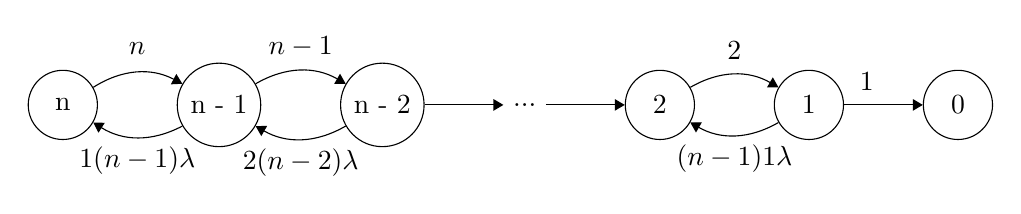
\begin{tikzpicture}[
   start chain = going right,
   -Triangle,
   every loop/.append style = {-Triangle}]
   \node[state, on chain]  (n) {n};
   \node[state, on chain]  (n1) {n - 1};
   \node[state, on chain]  (n2) {n - 2};
   \node[state without output/.append style={draw=none}, on chain]  (dots1) {...};
   \node[state, on chain]  (2) {2};
   \node[state, on chain]  (1) {1};
   \node[state, on chain]  (0) {0};

   \draw (n) edge[bend left] node[yshift=3mm]{$n$} (n1);
   \draw (n1) edge[bend left] node[yshift=-3mm]{$1 (n - 1) \lambda$}(n);

   \draw (n1) edge[bend left] node[yshift=3mm]{$n-1$} (n2);
   \draw (n2) edge[bend left] node[yshift=-3mm]{$2 (n - 2)\lambda$}(n1);

   \draw (n2) edge[left] node[xshift=3mm, yshift=-3mm]{} (dots1);

   \draw (dots1) edge[left] node[xshift=3mm, yshift=-3mm]{} (2);

  \draw (2) edge[bend left] node[yshift=3mm]{$2$} (1);
   \draw (1) edge[bend left] node[yshift=-3mm]{$(n - 1)1 \lambda$}(2);

  \draw (1) edge[left] node[yshift=3mm]{$1$} (0);
\end{tikzpicture}
    \caption{Transition rates for N node complete contact process}
    \label{fig:complete_contact_n_node_rates}
\end{figure}

In Figure \ref{fig:complete_contact_n_node_rates}, we show the transition rates for between the states of the contact process on the complete graph.
Note that for $i \in \{1, n - 1\} $ nodes that have a state of one, we have that the rate of going to $i + 1$ nodes is one of the $n - i$ nodes turning to one, each at a rate of $\lambda i$.
Thus, a total rate of $i (n - i) \lambda$.
The rate of going state with $i - 1$ ones is $i$ since we have $i$ nodes that have a potential to switch to zero, each with a rate of one.

Let $\tau_{C_n}$ be the time until we reach state zero.
Now let $N_1, N_2, \ldots, N_m$ be the number of visits to states $1, 2, \ldots, m$ respectively.
Let $X_i^{(n)} \sim \exp(n)$ be i.i.d random variables, $X_i^{(j)} \sim \exp(n - i + i(n - i)\lambda)$ for each $j \in \{1, \ldots, n-1\}$.
We can again represent $\tau_{C_n}$ as random sums

\begin{equation}\label{eq:wait_contact_sum}
    \tau_{C_n} = \sum_{i = 1}^{N_n} X_i^{(n)} + \sum_{i = 1}^{N_{n - 1}} X_i^{(n - 1)} + \cdots + \sum_{i = 1}^{N_1} X_i^{(1)}
\end{equation}

Since we are concerned with the limiting distribution we can instead focus on the rates up to a constant

\begin{theorem}
Let $N_k^{(n)}$ be a random variable that denotes the number of visits to state $k$ (that is, there are $k$ nodes with 1 with $n$ possible nodes) which is geometrically distributed. Then,
$$
E[N_k^{(n)}] = \begin{cases}
    O(\lambda^k) & k < n\\
    O(\lambda^{n - 1}) & k = n
\end{cases}
$$
\end{theorem}

\begin{proof}
We proceed by induction.
For the $k = 1$, we have that the parameter for $N_1^{(n)}$ is proportional to $\lambda$ since a success for the geometric distribution is going from state 1 to absorbing state 0.

Now assume that $k \not = n$ and will show it hold for $k + 1$.
Assume that $k + 1 \not = n$.
Then define geometric random variables $Y_1, Y_2, \ldots$ supported on $1,2,\ldots$ which denote the number of jumps from $k + 1$ to $k + 2$ before jumping to $k$.
Note that we do not care about what the system does after going to $k + 2$ since the state is guaranteed to return back to $k + 1$.
We have that $Y_i$ has a parameter proportional to $1/\lambda$.
Now let $M$ be another geometric random variable that represents the number of times that the process goes back to $k + 1$ from $k$.

It follows that
\begin{equation}
   N_{k + 1}^{(n)} = \sum_{i = 1}^M Y_i
\end{equation}

Then using Theorem \eqref{thm:geom_sum_geom}, we can conclude that $N_{k + 1}{(n)}$ is geometrically distributed with parameter proportional to $1/\lambda^{k + 1}$.
Thus, $E[N_{k + 1}^{(n)}] = O(1/\lambda^{k + 1})$

Then when $k = n$ case we note that $N_n \leq N_{n - 1}$ so that $E[N_{n}{(n)}] = O(\lambda^{n - 1})$.
\end{proof}

\begin{theorem}
Let $\tau_{C_n}$ be the waiting time until we reach state 1 in the $n$ node complete contact process.
The limiting distribution of $E[N_{n-1}^{(n)}]^{-1} \cdot \tau_{C_n}$ is an exponential distribution with parameter 1.
\end{theorem}

\begin{proof}
If we multiply Equation \eqref{eq:wait_contact_sum} by $E[N_{n-1}^{(n)}]^{-1}$ then for each $k < n$, by Theorem \eqref{thm:geom_sum_exp}, \eqref{thm:exp_scaling}, $E[N_{n-1}^{(n)}]^{-1} \sum_{i =
1}^{N_{k}} X_i^{(k)}$ will have a exponential distribution with parameter proportional to $\lambda^{n - k - 1}$ which approaches zero in distribution as $\lambda \to \infty$.

For $k = n$, we have that
$$
E[N_{n-1}^{(n)}]^{-1} \sum_{i =
1}^{N_{n}} X_i^{(n)} \Rightarrow \exp(1)
$$
as $\lambda \to \infty$.
\end{proof}

\subsection{Finite contact process on cycles}

Now we look at the finite contact process with a cycle (circle) configuration,$\Z/n$. The vertices are $\{1, 2,\ldots, n\}$, with edges between each $x$ and $y$ if $x \equiv y \pm 1 \mod n$.
Each node has an edge with exactly two other nodes.
For the two and three node case the graph is identical to the complete graph.

% TODO: Maybe draw tikz graph of the cycle?

\subsubsection{Four node cycle \texorpdfstring{$S_4$}{S4}}
We have $2^4 = 16$ possible configurations with four nodes.
We can combine some of these states which are equivalent under the contact process.
The state in the original process is denoted as a 4 character string of ones and zeros.
There is an edge between neighboring indices which wraps around so that the first and last digits are connected as well.

\begin{align*}
    \{1111\} &\to 4\\
    \{1110, 1101, 1011, 0111\} &\to 3\\
    \{1100, 0110, 0011, 1001\} &\to 2_t\\
    \{1010, 0101\} &\to 2_s\\
    \{1000, 0100, 0010, 0001\} &\to 1\\
    \{0000\} &\to 0
\end{align*}

It is easy to see that this is an equivalence relation that satisfies Theorem \ref{thm:mc_projection}.
The notation $2_t$ means two nodes with one where the ones have an edge between them (the $t$ is for together),
and $2_s$ are nodes where the two ones do not have an edge between them.

% \begin{figure}
%    \centering
%    \begin{tikzpicture}
%      \graph[circular placement, radius=4cm,
%         empty nodes, nodes={circle,draw}] {
%         a -- b;
%         b -- c;
%         c -- d;
%    };
%    \end{tikzpicture}
%    \caption{...}
    %\label{fig:_nodes_contact}
%\end{figure}

\begin{figure}[H]
    \centering
  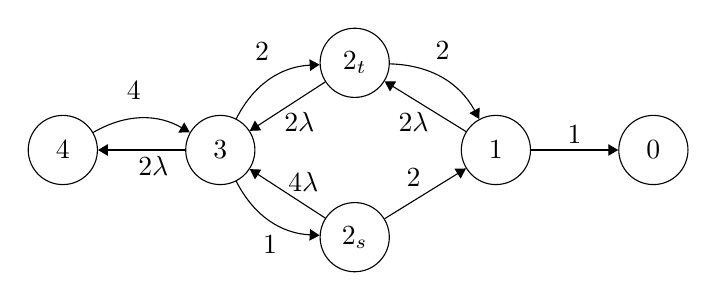
\begin{tikzpicture}[start chain = going right,
   -Triangle, every loop/.append style = {-Triangle}]
   \node[state, on chain]  (4) {4};
   \node[state, on chain]  (3) [right of=4]  {3};
   \node[state, on chain]  (2t) [above right of=3, yshift=4mm]  {$2_t$};

   \node[state, on chain]  (2s) [below right of=3, yshift=-4mm]  {$2_s$};
   \node[state, on chain]  (1) [right of=3, xshift=15mm]  {1};

   \node[state, on chain]  (0) [right of=1]  {0};


   \draw (4) edge [bend left] node[yshift=3.5mm, xshift=-1mm]{$4$} (3);
   \draw (3) edge [] node[yshift=-2mm, xshift=1.5mm]{$2 \lambda$} (4);

    \draw (3) edge [bend left] node[yshift=3.5mm, xshift=-1mm]{$2$} (2t);
   \draw (2t) edge [] node[yshift=-2mm, xshift=1.5mm]{$2 \lambda$} (3);

   \draw (3) edge [bend right] node[yshift=-3mm]{$1$} (2s);
   \draw (2s) edge [] node[yshift=1.5mm, xshift = 2mm]{$4\lambda$} (3);

    \draw (2t) edge [bend left] node[yshift=3.5mm]{$2$} (1);
   \draw (1) edge [] node[yshift=-2mm, xshift=-1.5mm]{$2\lambda$} (2t);

   \draw (2s) edge [] node[yshift=2mm, xshift=-1.5mm]{$2$} (1);

   \draw (1) edge [] node[yshift=2mm]{$1$} (0);

\end{tikzpicture}
    \caption{Projected rates of four node contact process on cycle}
    \label{fig:four_node_contact_cycle}
\end{figure}

\begin{equation}
Q_{S_4} =
\begin{blockarray}{ccccccc}
    & 4 & 3 & 2_t & 2_s & 1 & 0\\
    \begin{block}{c|cccccc}
    \cline{2-7}
    4 & -4 & 4 & 0 & 0 & 0 & 0\\
    3 & 2\lambda & -(2\lambda + 3) & 2 & 1 & 0 & 0\\
    2_t & 0 & 2\lambda & -(2\lambda + 2) & 0 & 2 & 0\\
    2_s & 0 & 4\lambda & 0 & -(4\lambda + 2) & 2 & 0\\
    1 & 0 & 0 & 2\lambda & 0 & -(2\lambda + 1) & 1\\
    0 & 0 & 0 & 0 & 0 & 0 & 0\\
    \end{block}
\end{blockarray}
\end{equation}

% TODO: See if better way to do this
% Increase spacing between row
% \begingroup
% \renewcommand*{\arraystretch}{2}
% \begin{equation}
% P_{S_4} =
% \begin{blockarray}{ccccccc}
%     & 4 & 3 & 2_t & 2_s & 1 & 0\\
%     \begin{block}{c|ccccc|c}
%     \cline{2-7}
%     4 & 0 & 1 & 0 & 0 & 0 & 0\\
%     3 & \frac{2\lambda}{2\lambda + 3} & 0 & \frac{2}{2\lambda + 3} & \frac{1}{2\lambda + 3} & 0 & 0\\
%     2_t & 0 & \frac{\lambda}{\lambda + 1} & 0 & 0 & \frac{1}{\lambda + 1} & 0\\
%     2_s & 0 & \frac{2\lambda}{2\lambda + 1} & 0 & 0 & \frac{1}{2\lambda + 1} & 0\\
%     1 & 0 & 0 & \frac{2\lambda}{2\lambda + 1} & 0 & 0 & \frac{1}{2\lambda + 1}\\
%     \cline{2-6}
%     \end{block}
%     \begin{block}{c|cccccc}
%     0 & 0 & 0 & 0 & 0 & 0 & 1\\
%     \end{block}
% \end{blockarray}
% \end{equation}

% Let $B_{S_4}$ be the transient states from $P_{S_4}$ which are inside the inner box.

%\begin{gather}
%\notag
%\mathclap{
%    \begin{multlined}
%    I + B_{S_4} + B_{S_4}^2 + \cdots = (I - B_{S_4})^{-1} = \\
%    \begin{blockarray}{cccccc}
%    & 4 & 3 & 2_t & 2_s & 1\\
%    \begin{block}{c|ccccc}
%    \cline{2-6}
%    4 & \frac{8 \lambda^4 + 8 \lambda^3 + 6 \lambda^2 + 7 \lambda + 3}{5 \lambda + 3} & \frac{(2 \lambda + 1) (2 \lambda + 3) (2 \lambda^2 + \lambda + 1)}{5 \lambda + 3} & \frac{2 (\lambda + 1)^2 (4 \lambda + 1)}{5 \lambda + 3} & \frac{(2 \lambda + 1) (2 \lambda^2 + \lambda + 1)}{5 \lambda + 3} & 2 \lambda + 1
%\\
%    3 &   \frac{2 \lambda (2 \lambda + 1) (2 \lambda^2 + \lambda + 1)}{5 \lambda + 3} & \frac{(2 \lambda + 1) (2 \lambda + 3) (2 \lambda^2 + \lambda + 1)}{5 \lambda + 3} & \frac{2 (\lambda + 1)^2 (4 \lambda + 1)}{5 \lambda + 3} & \frac{(2 \lambda + 1) (2 \lambda^2 + \lambda + 1)}{5 \lambda + 3} & 2 \lambda + 1
%\\
%    2_t &   \frac{2 \lambda^2 (2 \lambda + 1)^2}{5 \lambda + 3} & \frac{\lambda (2 \lambda + 1)^2 (2 \lambda + 3)}{5 \lambda + 3} & \frac{(\lambda + 1) (2 \lambda + 1) (4 \lambda + 3)}{5 \lambda + 3} & \frac{\lambda (2 \lambda + 1)^2}{5 \lambda + 3} & 2 \lambda + 1
%\\
%    2_s &   \frac{4 \lambda^2 (2 \lambda^2 + 2 \lambda + 1)}{5 \lambda + 3} & \frac{2 \lambda (2 \lambda + 3) (2 \lambda^2 + 2 \lambda + 1)}{5 \lambda + 3} & \frac{2 \lambda (\lambda + 1) (4 \lambda + 5)}{5 \lambda + 3} & \frac{(2 \lambda + 1) (2 \lambda^2 + \lambda + 3)}{5 \lambda + 3} & 2 \lambda + 1
%\\
%    1 &   \frac{4 \lambda^3 (2 \lambda + 1)}{5 \lambda + 3} & \frac{2 \lambda^2 (2 \lambda + 1) (2 \lambda + 3)}{5 \lambda + 3} & \frac{2 \lambda (\lambda + 1) (4 \lambda + 3)}{5 \lambda + 3} & \frac{2 \lambda^2 (2 \lambda + 1)}{5 \lambda + 3} & 2 \lambda + 1
%\\
%    \end{block}
%\end{blockarray}
%\end{multlined}
%    }
%\end{gather}
%\endgroup

% The top row of this matrix indicates the expected number of visits to each state when starting at state 4 (all ones configuration).

\subsubsection{Phase-type Distribution}

In Figure \ref{fig:contact_4_cycle_phase_densities} we plot the density functions for $\tau_{S_4}$ for $\lambda = 1, 2, 3, 4$ on the four node contact process on a cycle.

\begin{figure}[H]
  \centering
    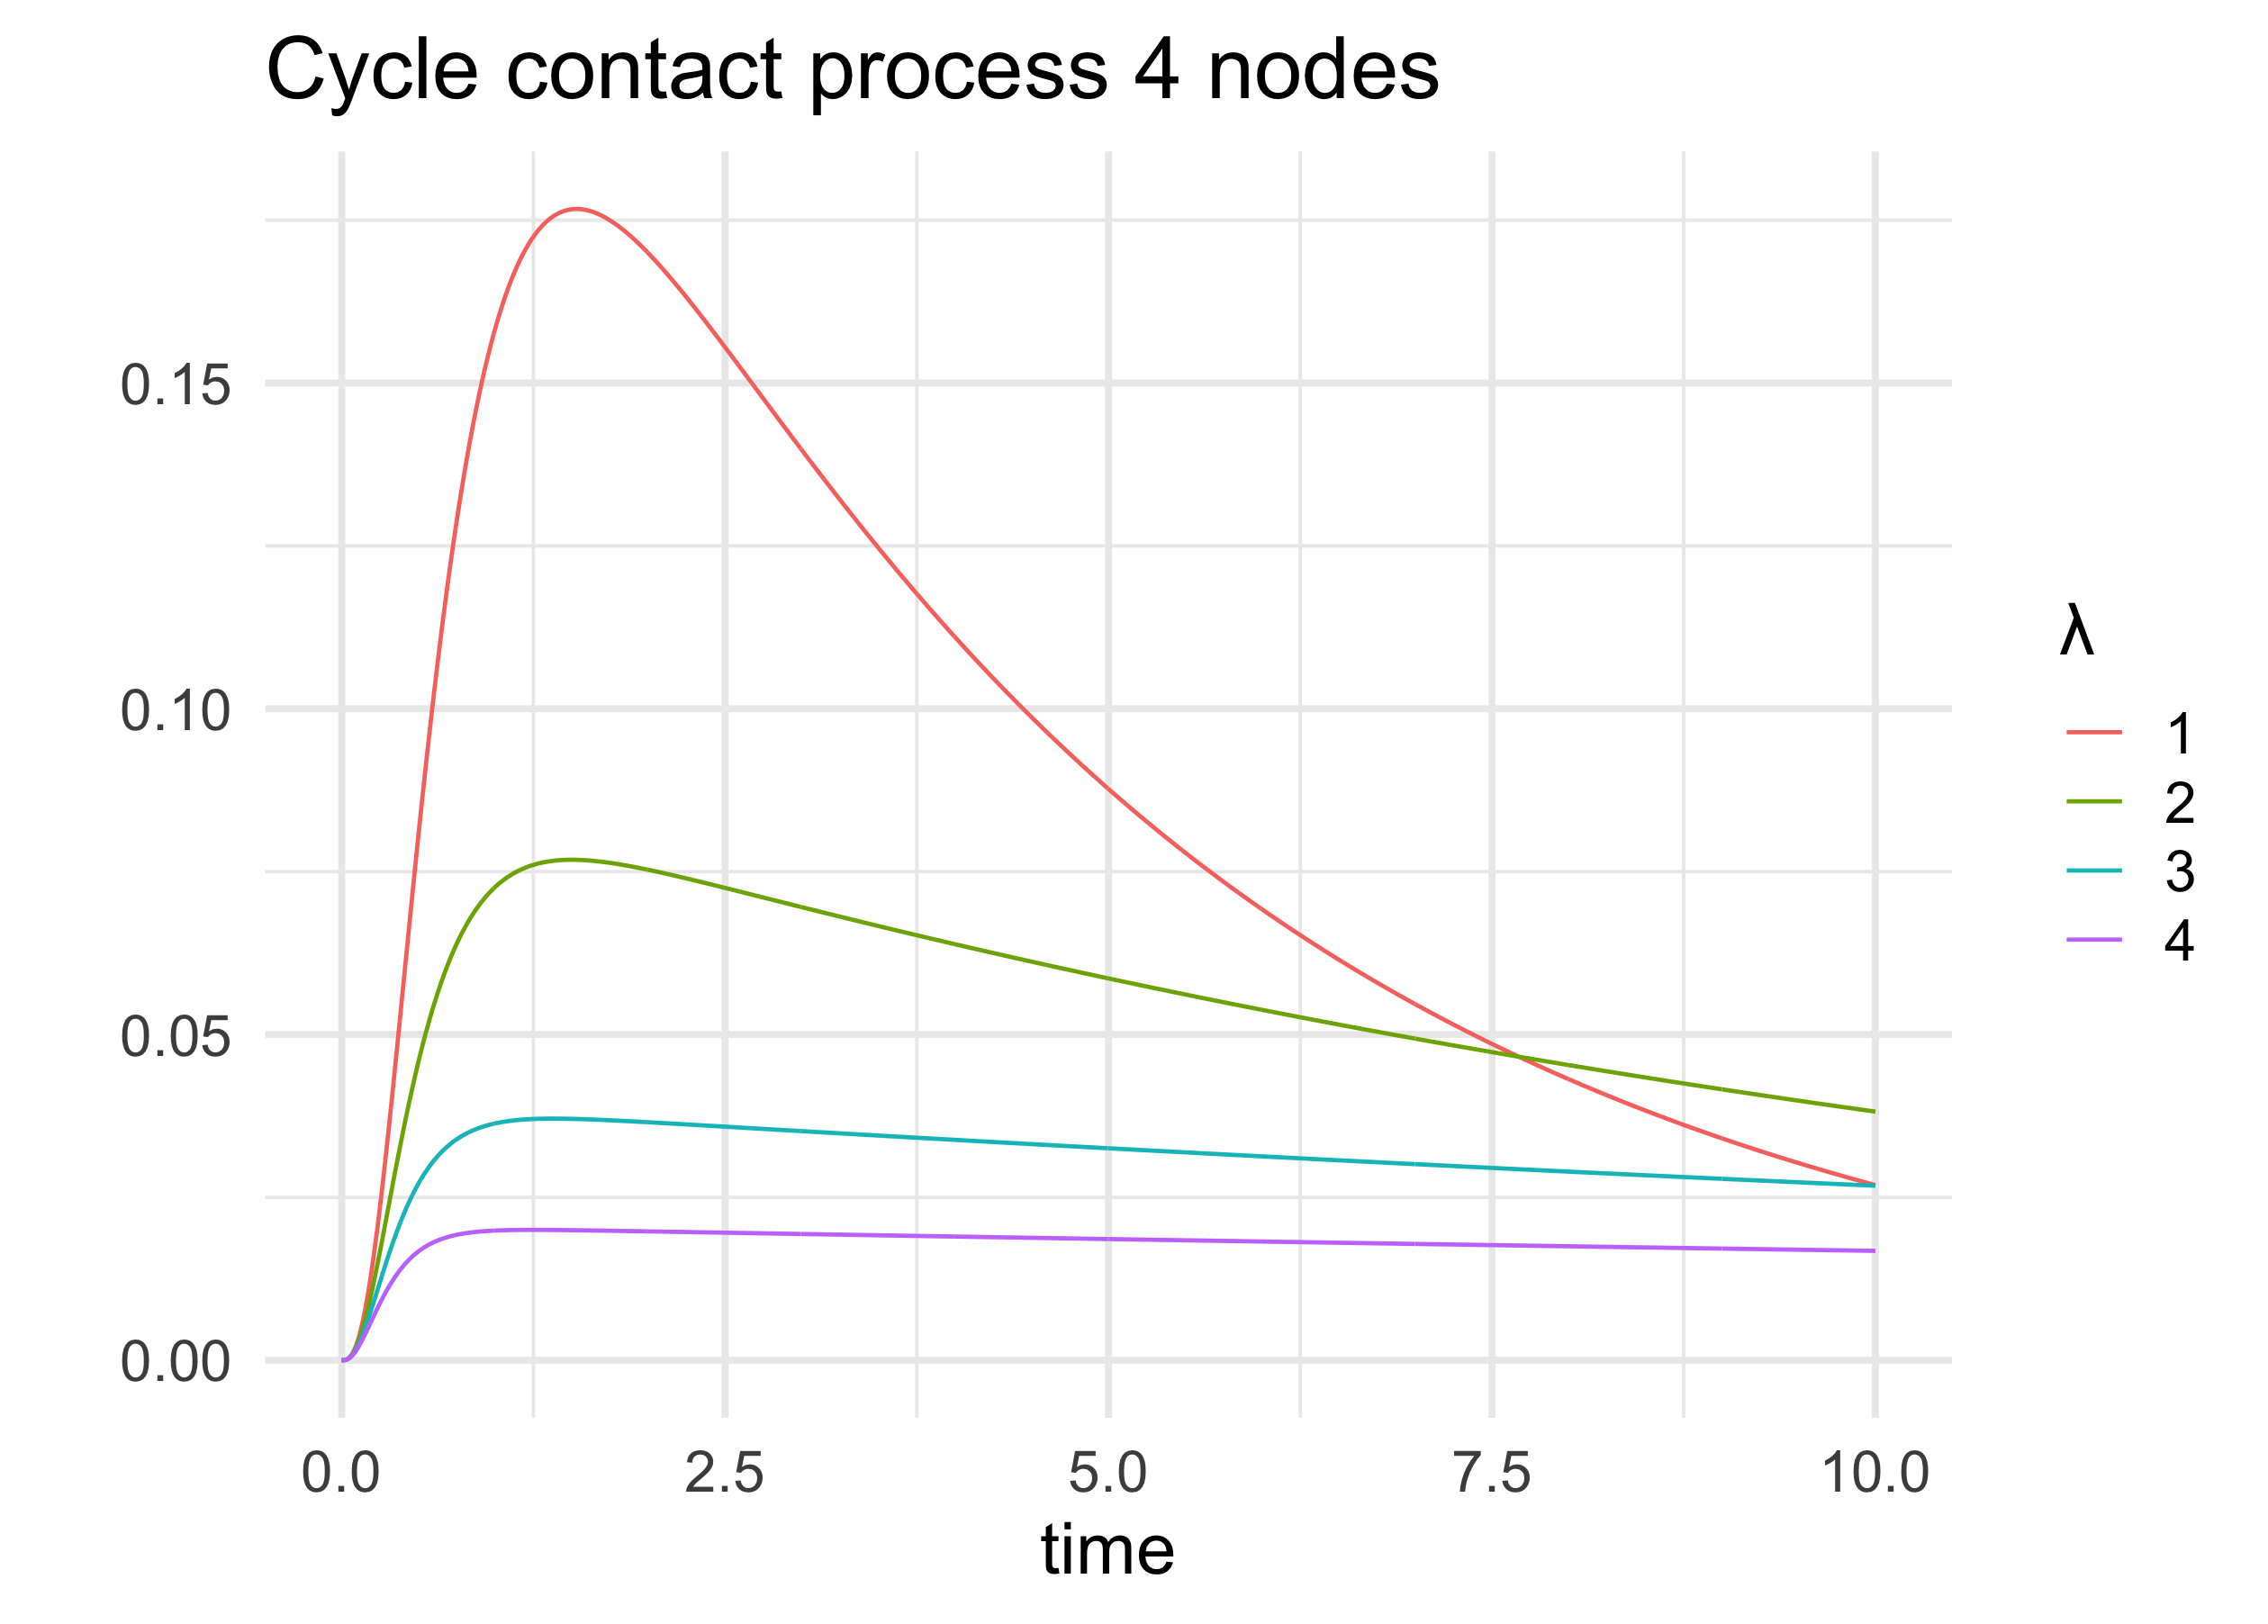
\includegraphics[width=.80\textwidth]{figures/cycle_4_contact_phase_densities.png}
   \caption{Density functions for $\tau_{S_4}$ for $\lambda = 1, 2, 3, 4$ on the four node contact process on a cycle}
  \label{fig:contact_4_cycle_phase_densities}
\end{figure}

\subsection{Finite contact process on 1D lattice}

Now we look at a contact process on a finite subset of a 1-dimensional lattice.
That is, two nodes will have exactly one edge while the rest will have two edges.
This is in contrast to the cycle which has exactly two edges for each node.
The two node contact process on the lattice is identical to the complete graph.

\subsubsection{Three node contact process \texorpdfstring{$L_3$}{L3}}
We can project the three node contact process with two edges onto a new Markov chain by Theorem \ref{thm:mc_projection} by associating states 110 and 011 as well as 100 and 001.
For the three node contact process with two edges, we have a transition graph shown in Figure \ref{fig:three_node_contact_lattice_states}.

\begin{figure}[H]
    \centering
   %\begin{tikzpicture}[auto, node distance=2cm, every loop/.style={-Triangle}, thick,main node/.style={circle,draw}]
  \begin{tikzpicture}[start chain = going right,
   -Triangle, every loop/.append style = {-Triangle}]
   \node[state, on chain]  (111) {111};
   \node[state, on chain]  (110) [above right of=111, yshift = 4mm]  {110};
   \node[state, on chain]  (101) [below right of=111, yshift = -4mm]  {101};

   \node[state, on chain]  (010) [right of=110, xshift=3mm]  {010};
   \node[state, on chain]  (100) [right of=101, xshift=3mm]  {100};

   \node[state, on chain]  (000) [below right of=010]  {000};


   \draw (111) edge [bend left] node[yshift=3.5mm, xshift=-1mm]{$2$} (110);
   \draw (110) edge [] node[yshift=-2mm, xshift=1.5mm]{$\lambda$} (111);

   \draw (111) edge [bend right] node[yshift=-3mm]{$1$} (101);
   \draw (101) edge [] node[yshift=1.5mm, xshift = 2mm]{$2\lambda$} (111);

   \draw (110) edge [bend left] node[yshift=3mm]{$1$} (010);
   \draw (010) edge [] node[yshift=-2mm, xshift=1.5mm]{$2 \lambda$} (110);

   \draw (101) edge [] node[yshift=-3mm]{$2$} (100);

   \draw (110) edge [] node[yshift=3mm]{$1$} (100);
   \draw (100) edge [bend left] node[yshift=3mm]{$\lambda$} (110);

  \draw (010) edge [] node[yshift=3mm]{$1$} (000);
  \draw (100) edge [] node[yshift=-3mm]{$1$} (000);

\end{tikzpicture}
    \caption{Three node contact process on 1D lattice projected rates between each states}
    \label{fig:three_node_contact_lattice_states}
\end{figure}

\begin{equation}
Q_{L_3} =
\begin{blockarray}{ccccccc}
    & 111 & 110 & 101 & 100 & 010 & 000\\
    \begin{block}{c|cccccc}
    \cline{2-7}
    111 & -3 & 2 & 1 & 0 & 0 & 0\\
    110 & \lambda & -(\lambda + 2) & 0 & 1 & 1 & 0\\
    101 & \lambda & 0 & -(\lambda + 1) & 1 & 0 & 0\\
    100 & 0 & \lambda & 0 & -(\lambda + 1) & 0 & 1\\
    010 & 0 & 2\lambda & 0 & 0 & -(2\lambda + 1) & 1\\
    000 & 0 & 0 & 0 & 0 & 0 & 0\\
    \end{block}
\end{blockarray}
\end{equation}

\subsubsection{Phase-type Distribution}

In Figure \ref{fig:lattice_3_contact_phase_densities} we plot the density functions for $\tau_{L_3}$ for $\lambda = 1, 2, 3, 4$ on the four node contact process on a cycle.

\begin{figure}[H]
  \centering
    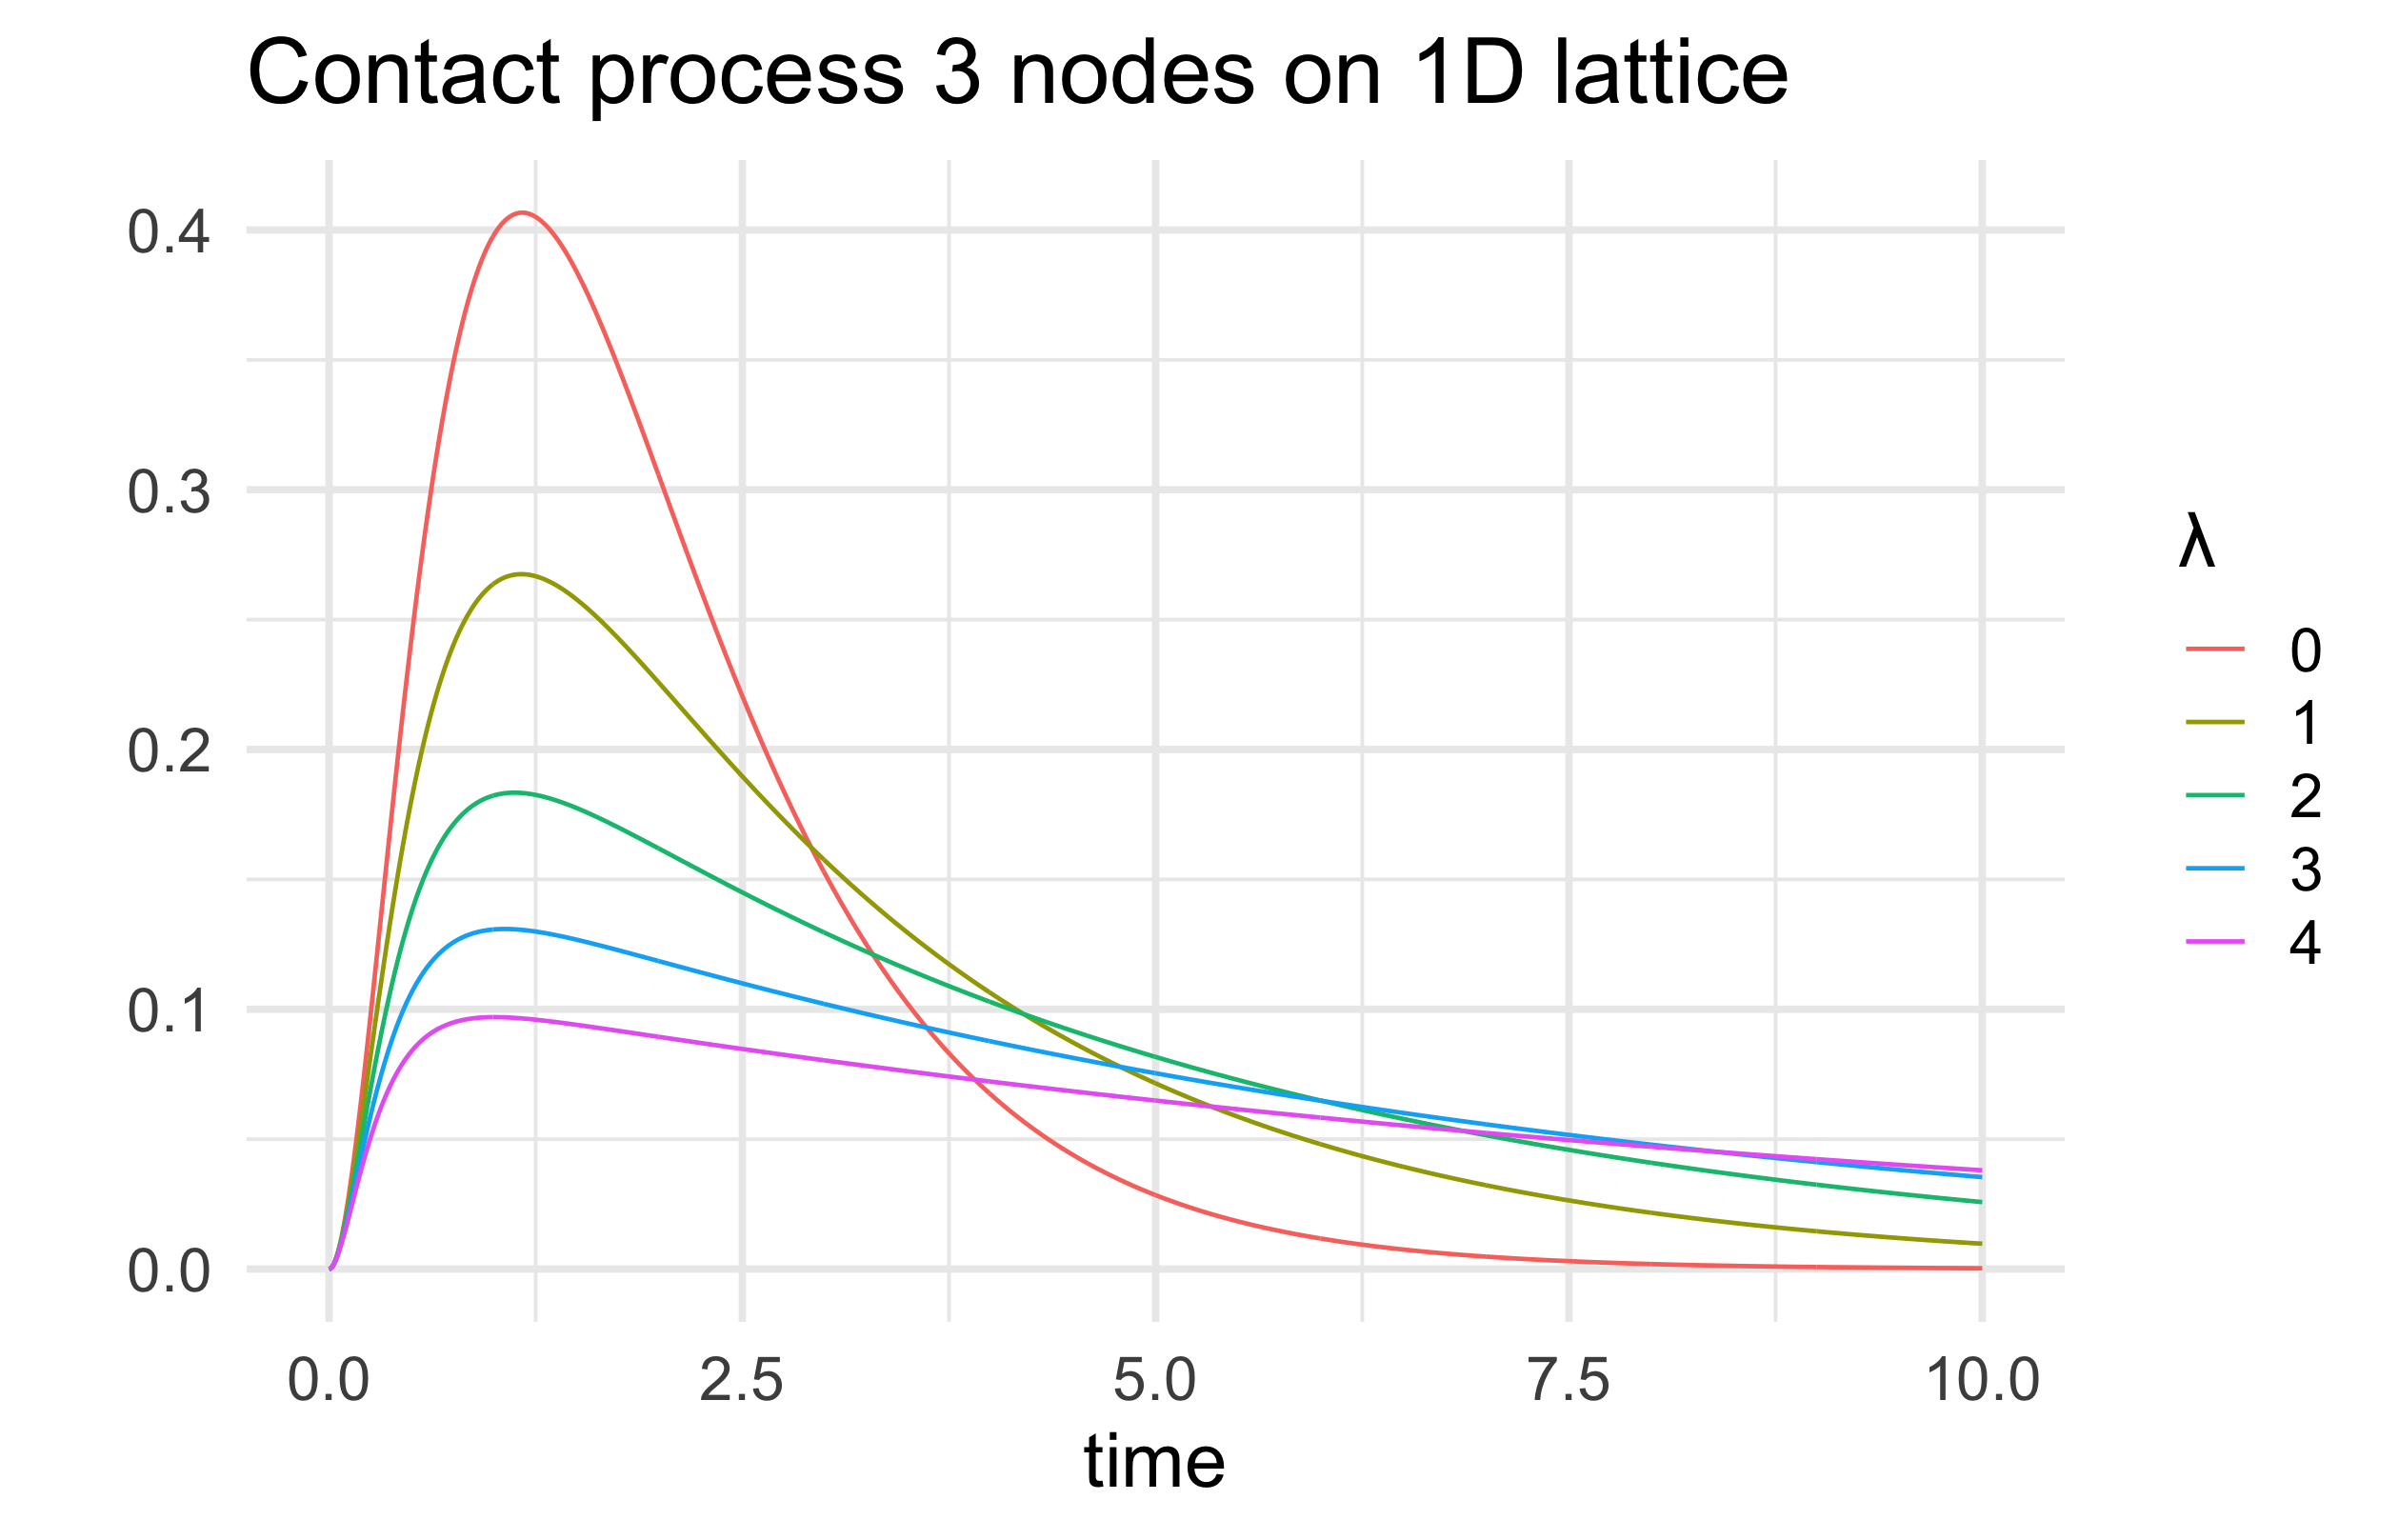
\includegraphics[width=.80\textwidth]{figures/lattice_3_contact_phase_densities.png}
   \caption{Density functions for $\tau_{L_3}$ for $\lambda = 1, 2, 3, 4$ on the four node contact process on a cycle}
  \label{fig:lattice_3_contact_phase_densities}
\end{figure}

\subsection{Comparison of Phase-type distributions for \texorpdfstring{$C_2$}{C2}, \texorpdfstring{$C_3$}{C3}, \texorpdfstring{$L_3$}{L3}, and \texorpdfstring{$S_4$}{S4}}

All of the graph configurations are identical when we have two nodes.
Also, $S_3$ is the same as $C_3$.
In Figure \ref{fig:ev_phase_comparison_3.png} we compare of expected values of $\tau_{C_2}$, $\tau_{C_3}$, and $\tau_{L_3}$.
Since $\tau_{S_4}$ is much larger than $\tau_{C_2}$, $\tau_{C_3}$, and $\tau_{L_3}$ we include it separately in Figure \ref{fig:ev_phase_comparison_4.png}.

\begin{figure}[H]
  \centering
    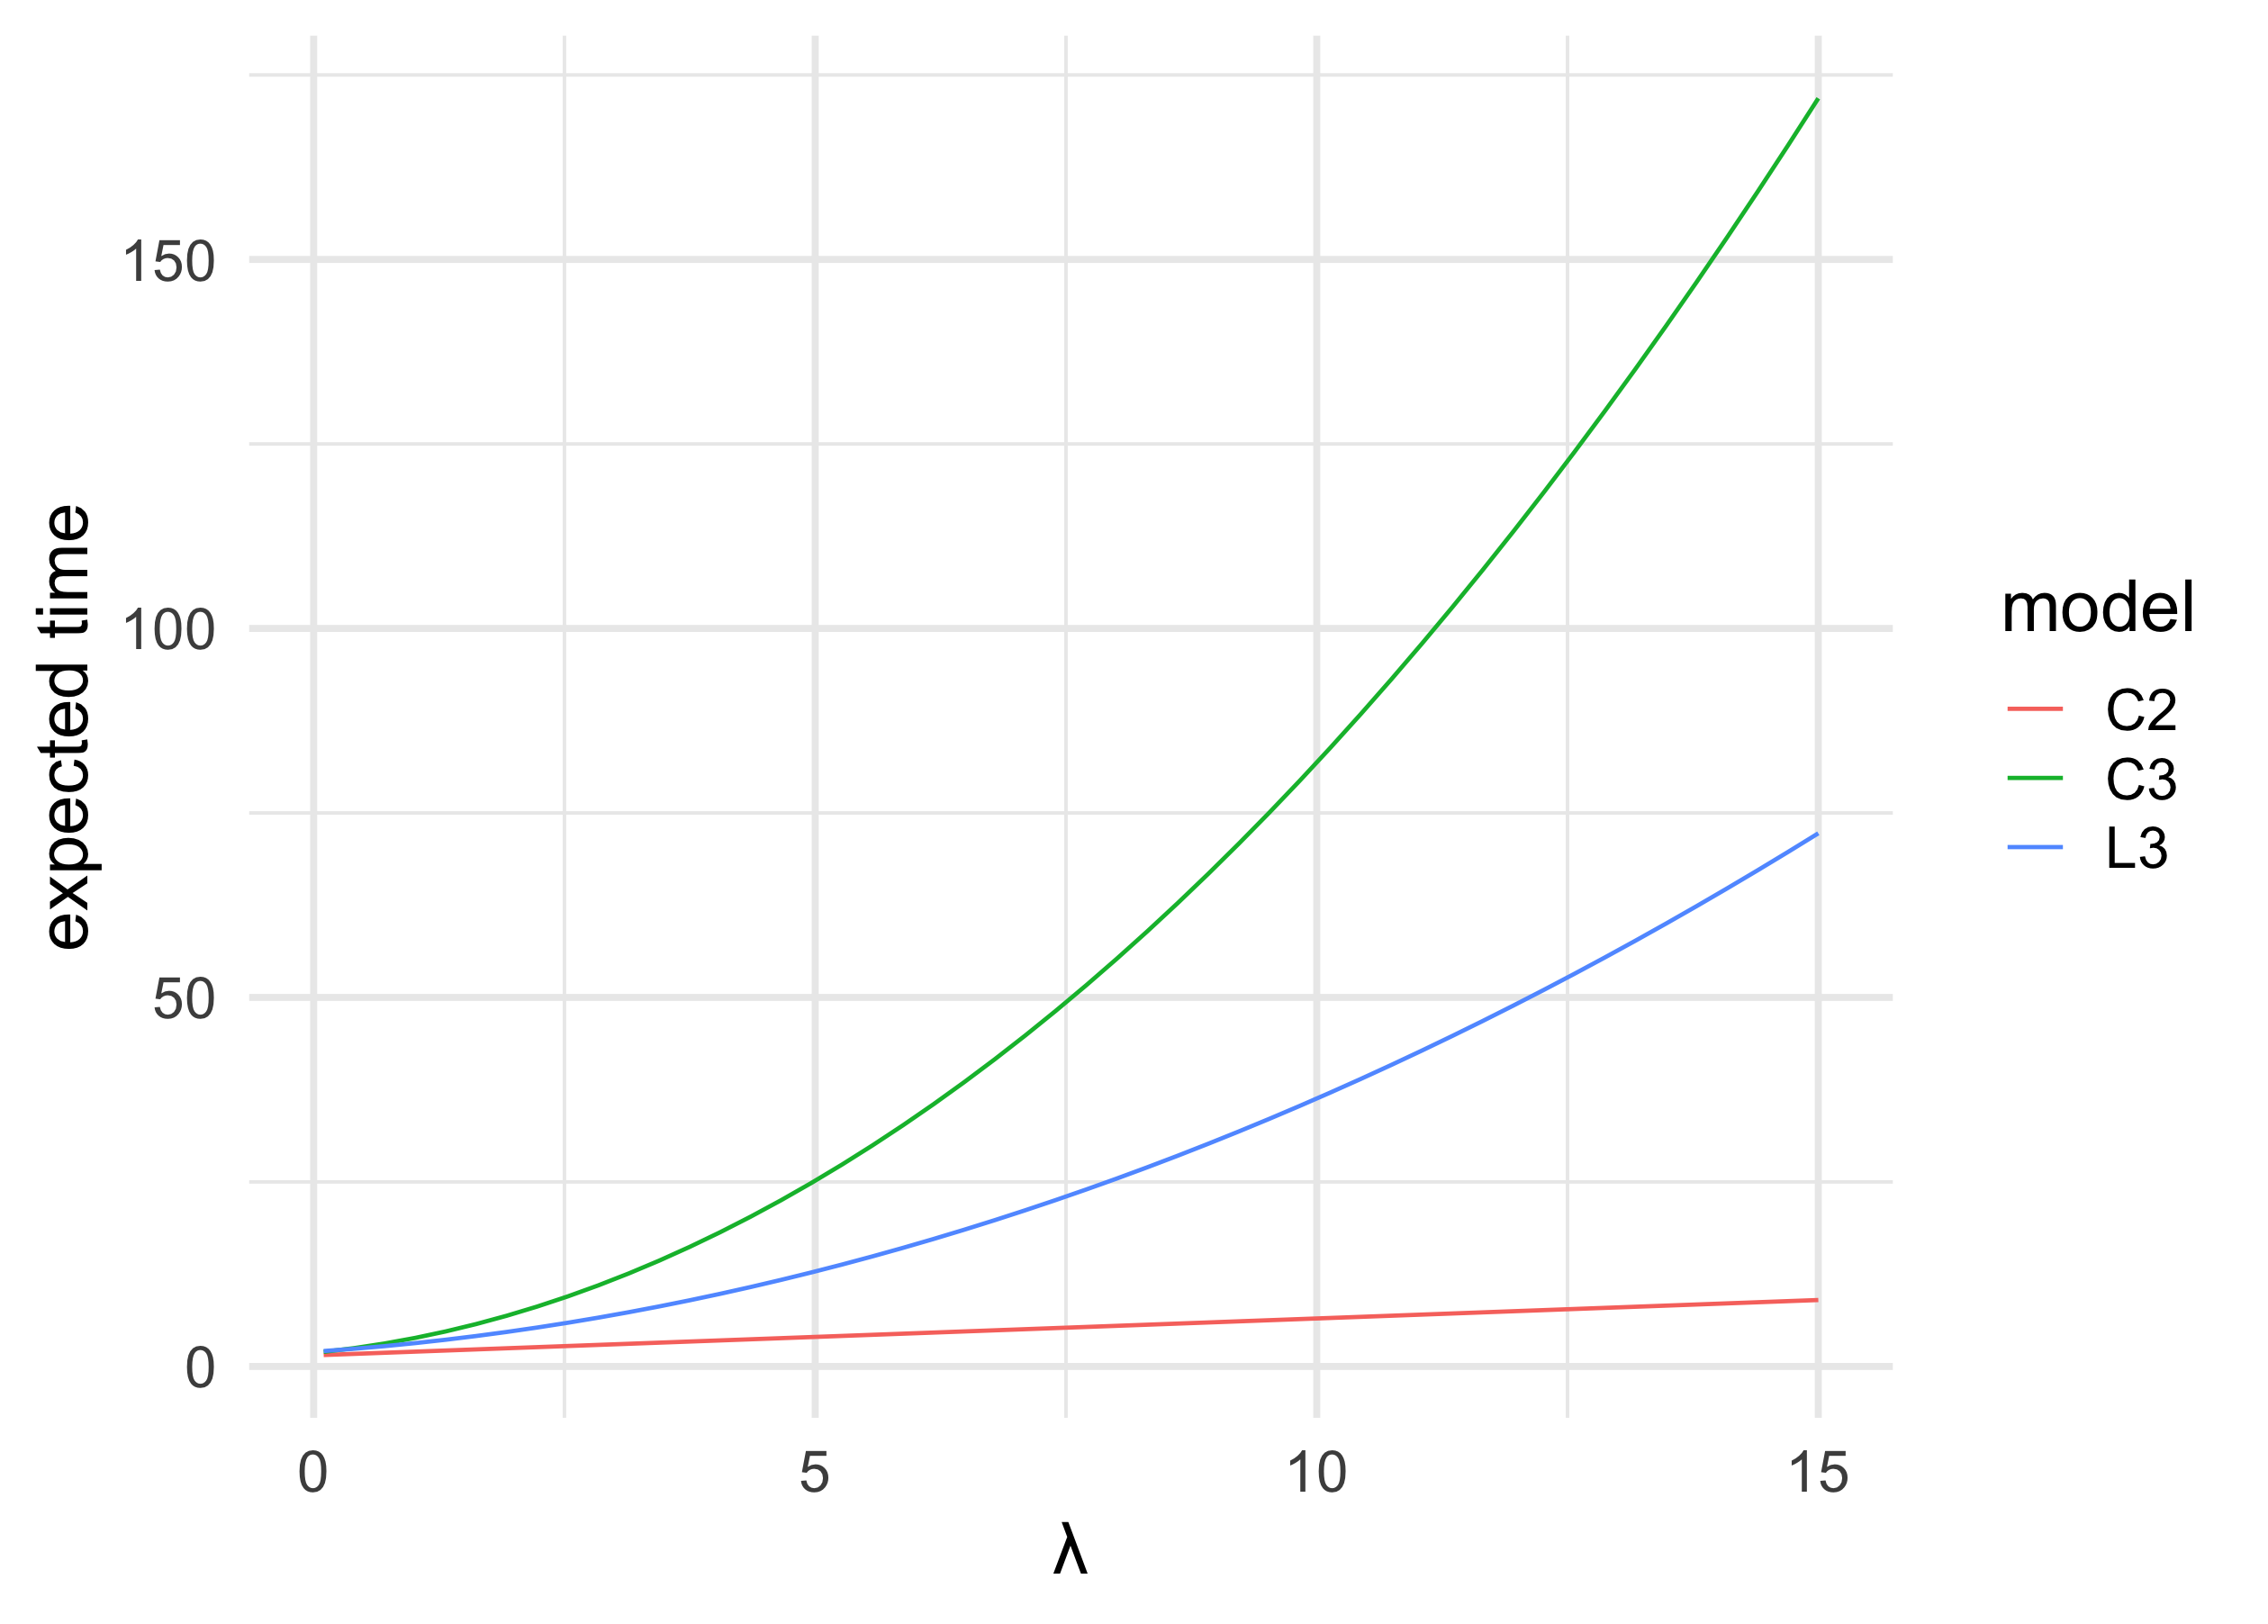
\includegraphics[width=.80\textwidth]{figures/ev_phase_comparison_3.png}
   \caption{Comparison of expected values of $\tau_{C_2}$, $\tau_{C_3}$, and $\tau_{L_3}$}
  \label{fig:ev_phase_comparison_3.png}
\end{figure}

\begin{figure}[H]
  \centering
    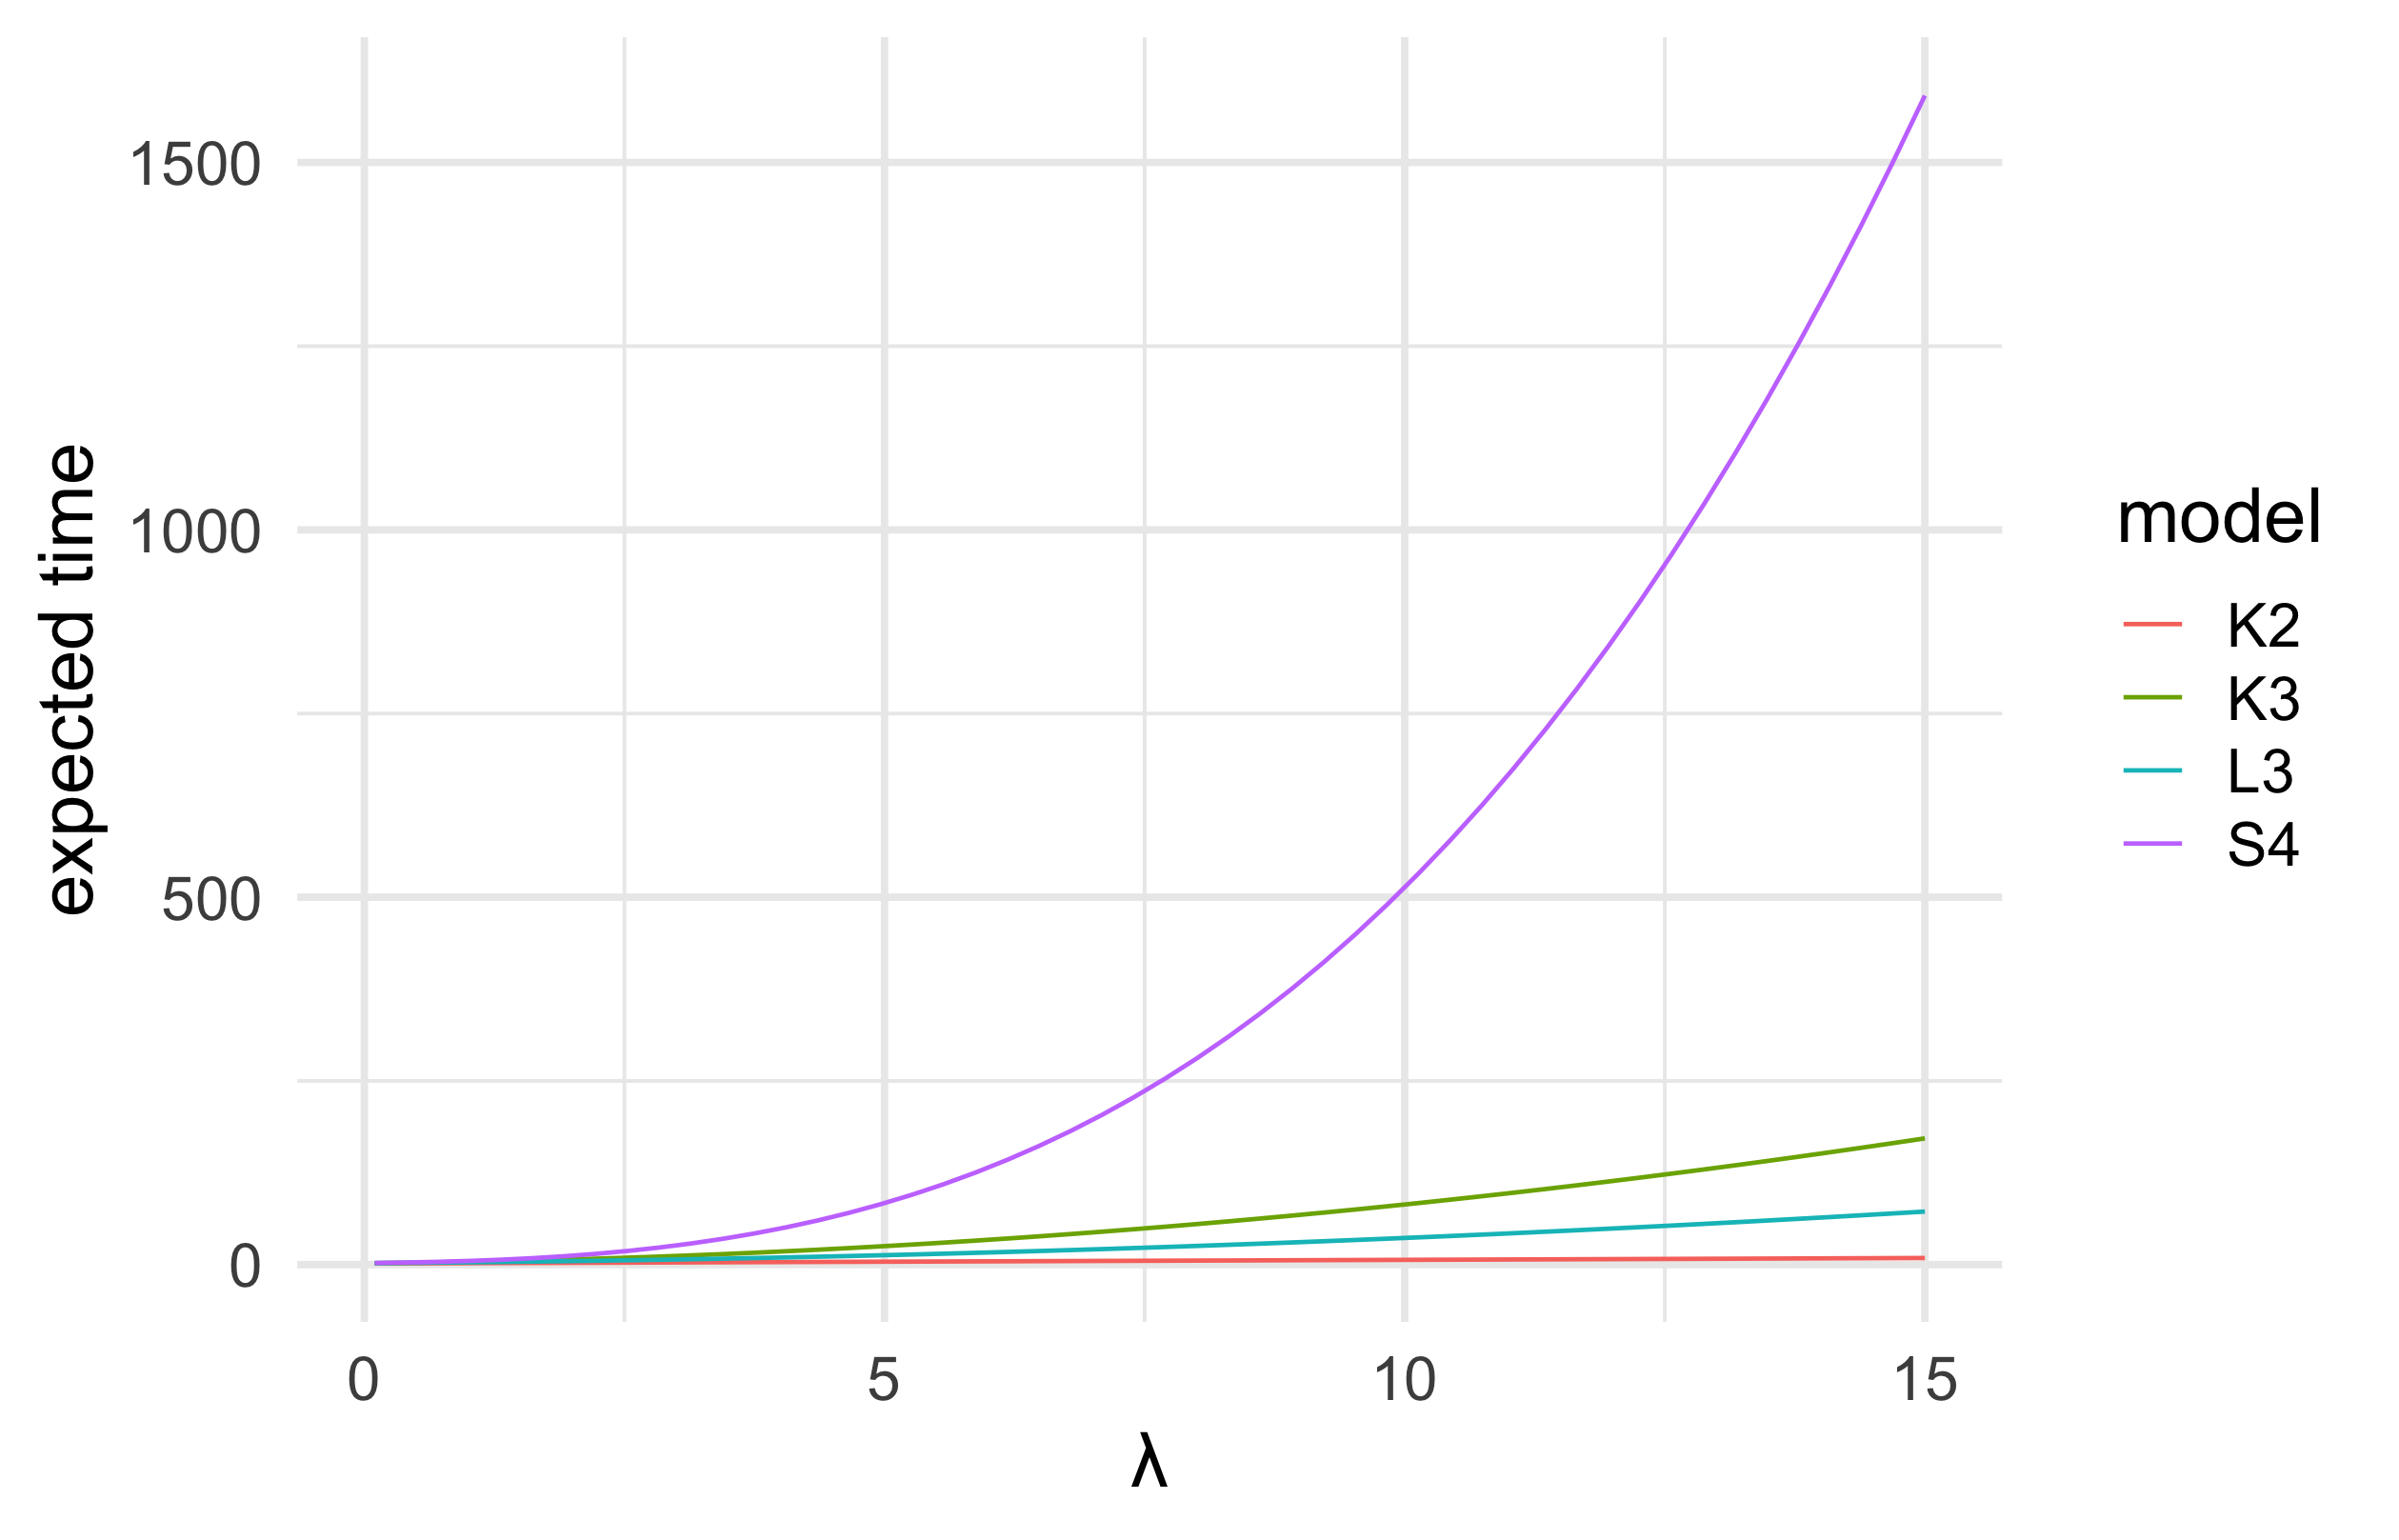
\includegraphics[width=.80\textwidth]{figures/ev_phase_comparison_4.png}
   \caption{Comparison of expected values of $\tau_{C_2}$, $\tau_{C_3}$, $\tau_{L_3}$, and $\tau_{S_4}$}
  \label{fig:ev_phase_comparison_4.png}
\end{figure}

\subsection{Simulation of contact process on \texorpdfstring{$\Z^2$}{Z2}}
In this section we describe how to simulate the linear voter model on the two-dimensional lattice $\Z^2$.
By nature of the simulation we have to restrict $\Z^2$ to some finite subset of $\Z^2$.
A new issue then arises with the boundaries.
To capture the finite behavior of the system it makes sense to just keep the boundaries nodes with a reduced number of edges.
If we want to simulate the behavior on $\Z^2$ then it is better to use \textit{periodic boundary conditions} where we let the state space be $\{0,1\}^{(\Z/n)^2}$ where $n$ is some finite number.
This means that each node on the graph will have exactly

The dynamics of the system are that each 1 waits exponential time with rate 1 and changes to 0.
Each 1 waits an independent exponential time with rate $\lambda$ and then places a 1 onto one of the $d$ neighbors with probability $1/2^d$.
If there already is a 1 at this spot then nothing happens.
\cite{steif91}

\section{Voter Model}

\begin{defn}[Voter Model] \cite{Liggett2002}
Let $\Z^d$ be the state space and $P$ be the transition probability matrix for a Markov chain on $S$.
Then $\Omega = \{0,1\}^{\Z^d}$ is the state space for voter model which is a continuous-time Markov chain.
For $\eta \in \Omega$ denote $\eta(x)$ as the value of the node $x \in \Z^d$ on the configuration $\eta$.
Let $\eta_x$ be the configuration from changing the value of $\eta$ at the site $x$. That is,
$$
\eta_x(y) = \begin{cases}
    \eta(y) & x \not = y\\
    1 - \eta(y) & x = y
\end{cases}
$$
The transition rates $Q$ are defined as
$$
q(\eta, \eta_x) = \sum_{y : \eta(y) \not = \eta(x)} P(x,y)
$$
Thus, for any $\eta, \delta \in \Omega$ that differ by more than one sites,
$$
q(\eta, \delta) = 0
$$

In general we assume that on $Z^d$ then $P(x,y) = P(0, x - y)$. Where $P(x- y) = \frac{1}{2d}$ if $x$ and $y$ are adjacent and $P(x-y) = 0$ otherwise.

The transition rates have the following properties:
\begin{enumerate}
    \item $q(\eta, \eta_x) = 0$ for each $x \in \Z^d$ if $\eta \equiv 0$ or $\eta \equiv 1$
    \item $q(\eta, \eta_x) = q(\zeta, \zeta_x)$ for every $x \in \Z^d$ if $\eta(y) + \zeta(y) = 1$ for all $y \in \Z^d$. That is, the dynamics of the system are not changed by interchanging 1 and 0.
    \item $q(\eta, \eta_x) \leq q(\zeta, \zeta_x)$ if $\eta \leq \zeta$ and $\eta(x) = \zeta(x) = 0$
    \item $q(\eta, \eta_x)$ is invariant under shifts in $\Z^d$.
\end{enumerate}
\end{defn}

\begin{theorem}[\cite{Liggett1999}]
For $d = 1,2$ the voter model on $\Z^d$ with any initial configuration then
$$
\lim_{t \to \infty} P(\eta_t(x) \not = \eta_t(y)) = 0
$$
for all $x,y \in \Z^d$.
This behavior is called \textbf{clustering}.
\end{theorem}

In Figure \ref{fig:voter_sim_1d_torus.png} we show one realization from a simulation of the voter model with periodic boundaries on length 300 subset of $\Z$.
In Figure \ref{fig:voter_sim_2d_torus.png} we show one realization from a simulation of the voter model with periodic boundaries on a $100 \times 100$ grid.

\begin{figure}[H]
  \centering
    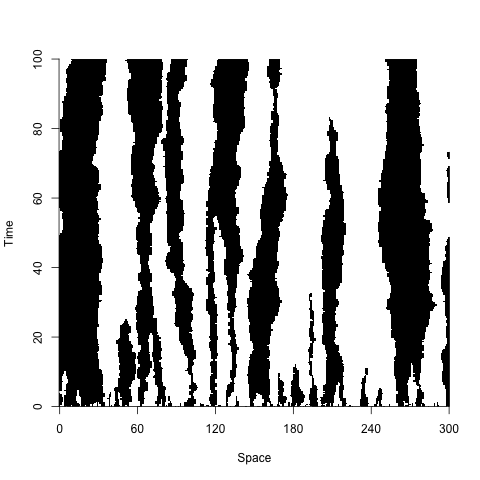
\includegraphics[width=.80\textwidth]{figures/voter_simulation_1d_300.png}
   \caption{Simulation for voter model with periodic boundary conditions on length 300 subset of $\Z$}
  \label{fig:voter_sim_1d_torus.png}
\end{figure}

\begin{figure}[H]
  \centering
    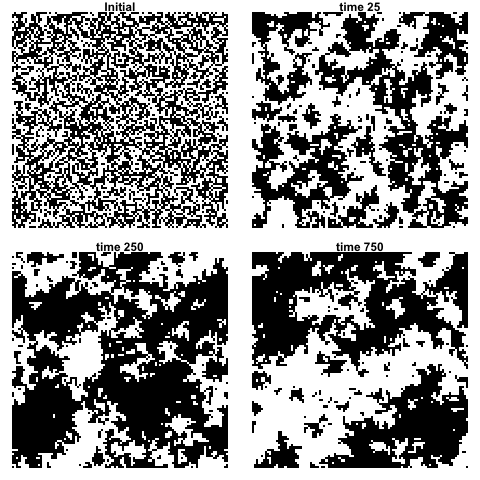
\includegraphics[width=.80\textwidth]{figures/voter_simulation_torus_100.png}
   \caption{Simulation for voter model with periodic boundary conditions on $100 \times 100$ grid.}
  \label{fig:voter_sim_2d_torus.png}
\end{figure}

\subsection{Finite Linear Voter Model}
We will now look at the time for linear voter model on a finite cycle and complete graph to reach the configuration of all 1's or all 0's.
In general there are $2^n$ configurations for the cycle but many of these have the same rates due to rotations and the property that interchanging 1's and 0's are equivalent.
That is, if $\eta$ is a configuration then $1 - \eta$ should be in the same equivalence class.

In the complete graph each node in a configuration is connected to all of the others, we can project a configuration $\eta$ to the minimum number of ones in $\eta$ and $1 - \eta$.
$$
\eta \mapsto \min\left(|\{x : \eta(x) = 1\}|, |\{x : \eta(x) = 0\}|  \right)
$$
We will have $\lfloor n/2 \rfloor + 1$ new projected states for a voter model on a complete graph with $n$ nodes which will be a Markov chain
by \ref{thm:mc_projection}.

For all of the following models we will be using the following transition probability matrix
$$
P(x,y) = P(y,x) = \frac{1}{\deg(x)}
$$
Where $\deg(x)$ is the degree of the node $x$.
So in the case of the cycle, $P(x,y) = 1/2$, and the complete graph with $n$ node $P(x,y) = 1/(n - 1)$.

\begin{figure}[H]
  \centering
    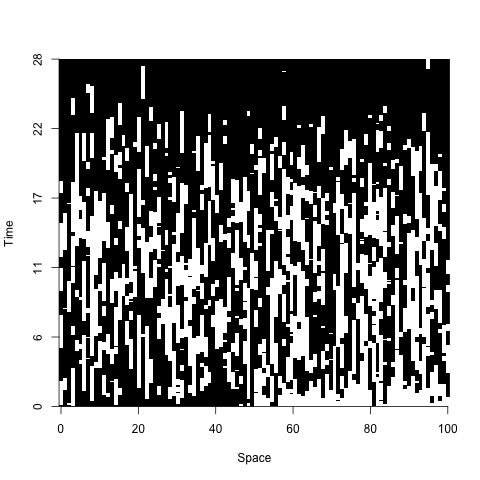
\includegraphics[width=.80\textwidth]{figures/voter_simulation_1d_complete_split_100.png}
   \caption{Simulation for voter model on a complete graph with 100 nodes. The initial configuration is split with half 1's and half 0's.}
  \label{fig:voter_sim_1d_complete.png}
\end{figure}

\subsubsection{Three node complete/cycle}
A complete graph (or a cycle) with $n = 3$ nodes has two projected states, $\{0,1\}$.
Assuming that we initialize the the voter model to state 1, then we will just wait unit exponential time before going to the absorbing state 0.

\subsection{Four node complete voter model \texorpdfstring{$C^{v}_4$}{VC4}}
The state space in the projected four node voter model is $\{0,1,2\}$.
When we are in state 2, then there are 4 possible nodes that can switch from 1 to 0 or 0 to 1.
Each of these switch at a rate of $2 \cdot 1/(4 - 1) = 2/3$ since they are connected to 2 other nodes with the opposite value.
Thus, the rate from $2 \to 1$ is $8/3$.
Similarly reasoning leads us to the rates in the form of the infinitesimal generator matrix
% 2 -> 1 rate 2 * 1/(4 - 1) * 2 = 4/3 is
$$
Q_{C^{v}_4} = \begin{blockarray}{cccc}
    & 2 & 1 & 0\\
    \begin{block}{c|ccc}
        \cline{2-4}
        2 & -\frac{8}{3} & \frac{8}{3} & 0 \\
        1 & 1 & -2 & 1\\
        0 & 0 & 0 & 0\\
    \end{block}
\end{blockarray}
$$
Let
\begin{align*}
    \mathbf{S} &= \begin{bmatrix}
    -\frac{8}{3} & \frac{8}{3}\\
    1 & -2\\
    \end{bmatrix}\\
    \mathbf{S}_0 &= (0, 1)^T
\end{align*}
Then the eigenvalues are determined by the characteristic polynomial
$$
(8/3 + m)(2 + m) - 8/3 = m^2 + \frac{14}{3} m + \frac{8}{3}
$$
which has roots of $m_1 = -4$ and $m_2 = - \frac{2}{3}$.
So the eigenvalues of $xS$ are $\lambda_1 = -4x$ and $\lambda_2 =  - \frac{2}{3} x$.
These eigenvalue have corresponding eigenvectors of $v_1 = (-2, 1)$ and $v_2 = (4/3, 1)$.
Let
$$
U = \begin{bmatrix}
    -2 & 4/3\\
    1 & 1
\end{bmatrix}
$$
thus
$$
U^{-1} = \frac{1}{10} \begin{bmatrix}
    -3 & 4\\
    3 & 6
\end{bmatrix}
$$
So the diagonalization of $S$ is given as
$$
\mathbf{S} = \begin{bmatrix}
    -2 & 4/3\\
    1 & 1
\end{bmatrix} \operatorname{diag}(-4x, - \frac{2}{3} x)
\frac{1}{10} \begin{bmatrix}
    -3 & 4\\
    3 & 6
\end{bmatrix}
$$
By Theorem \ref{thm:phase-type-pdf-cdf}, where $(\alpha_2, \alpha_1)$ is the probability of starting in state 2 and 1 respectively, we have the density of the absorption time $\tau_{C^{v}_4}$ is given as
\begin{align*}
    f_{C^{v}_4}(x) &= (\alpha_2, \alpha_1) \exp(x\mathbf{S}) \mathbf{S}_0\\
    &= \frac{1}{10} (\alpha_2, \alpha_1) \begin{bmatrix}
    -2 & 4/3\\
    1 & 1
\end{bmatrix}
\begin{bmatrix}
\exp(-4x) & 0\\
0 & \exp(- \frac{2}{3} x))
\end{bmatrix}
\begin{bmatrix}
    -3 & 4\\
    3 & 6
\end{bmatrix}
(0,1)^T\\
&= \frac{1}{10} (\alpha_2, \alpha_1)
\begin{bmatrix}
-2 \exp(-4x) & \frac{4}{3} \exp(-\frac{2}{3} x)\\
\exp(-4x) & \exp(- \frac{2}{3} x))
\end{bmatrix}
\begin{bmatrix}
    4\\
    6
\end{bmatrix}\\
&= \frac{1}{5} (\alpha_2, \alpha_1)
\begin{bmatrix}
-4 \exp(-4x) + 4 \exp(-\frac{2}{3} x)\\
2 \exp(-4x) + 3 \exp(-\frac{2}{3} x)
\end{bmatrix}\\
&= \frac{1}{5} \left[ \alpha_2 \left( -4 \exp(-4x) + 4 \exp\left(-\frac{2}{3} x\right) \right) + \alpha_1 \left( 2 \exp(-4x) + 3 \exp\left(-\frac{2}{3} x\right) \right) \right]\\
&= \frac{1}{5} \left[ (-4 \alpha_2 + 2 \alpha_1) \exp(-4x) + (4 \alpha_2 + 3 \alpha_1) \exp\left(-\frac{2}{3} x\right)\right]
\end{align*}

In Figure \ref{fig:voter_density_c4} we plot the density function for $\tau_{C^{v}_4}$ for varying $\boldsymbol{\alpha} = (\alpha_2, \alpha_1)$ values.
The expected value of $\tau_{C^{v}_4}$ is given by Theorem \ref{thm:phase-moments}
\begin{align*}
    E[\tau_{C^{v}_4}] &= -1 (\alpha_2, \alpha_1) \mathbf{S}^{-1} (1, 1)^T\\
    &= \frac{1}{8} (\alpha_2, \alpha_1) \begin{bmatrix}
    6 & 8\\
    3 & 8
    \end{bmatrix} (1,1)^T\\
    &= \frac{7}{4} \alpha_2 + \frac{11}{8} \alpha_1
\end{align*}
So when deterministically starting at state 2, we have that the expected value of the waiting time is $\frac{7}{4}$.

\begin{figure}[H]
  \centering
    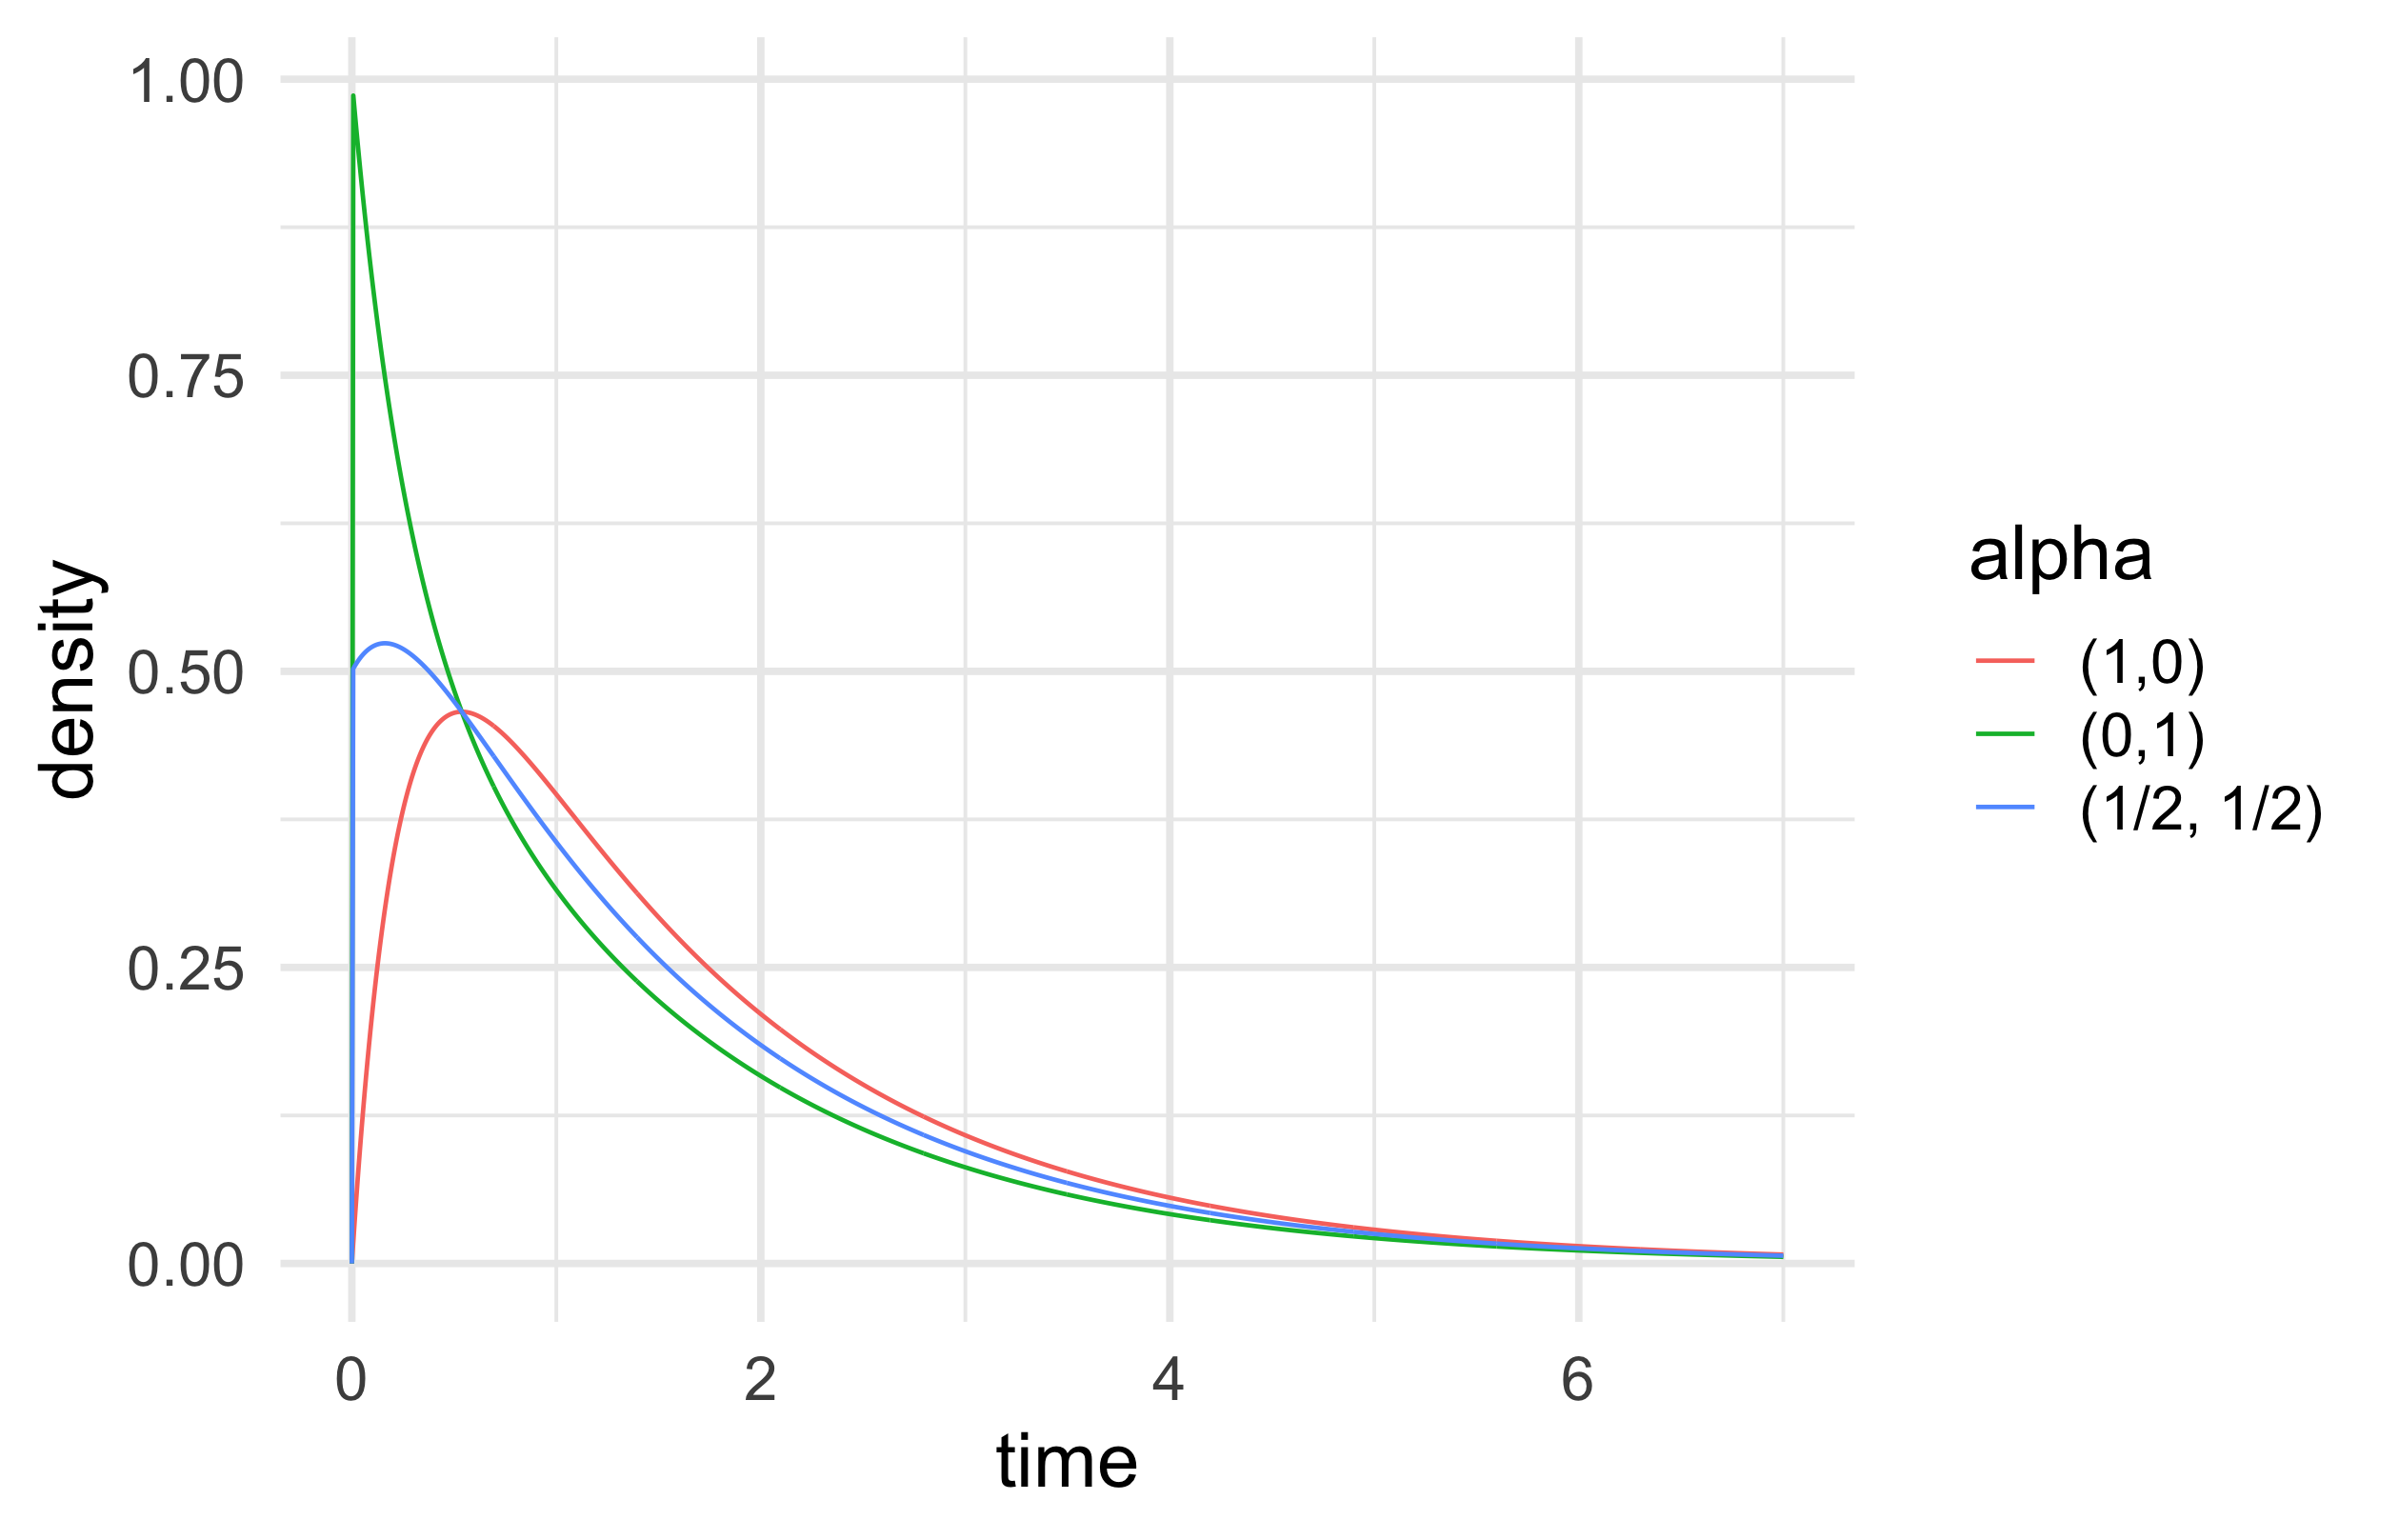
\includegraphics[width=.80\textwidth]{figures/voter_density_c4.png}
   \caption{Density of the absorption time for the voter model on the complete graph with four nodes, $C^{v}_4$. The initial stating position is varied between always stating at state $2$, starting at start $1$ and an equal mixture of starting at either 1 or 2.}
  \label{fig:voter_density_c4}
\end{figure}

\subsection{N node complete voter model}
If $N$ is even, then let $k = N / 2$ and if $N$ is odd then $k = (N - 1)/2$.
When $N$ is even we have $\{0,\ldots, N/2\}$ projected states.
Let $k = N/2$.
Assume we are in state $i \not = k$.
To transition to state $i + 1$, we have $n - i$ nodes that can flip to match the $i$ nodes.
Each one of these nodes will flip with a rate of $\frac{i}{n - 1}$ since the graph is complete and each node is connected to $i$ nodes with the opposite rate.
Thus, the rate is $(n - i) \frac{i}{n - 1}$.
Similarly for $i \to i - 1$ transition we have $i$ nodes that can flip at a rate of $\frac{n - i}{n - 1}$ leading to the same rate.
If $i = k$ then by symmetry we need to multiply the rate by $2$, since both the 1's or the 0's could switch.
We then multiply the rates by $(n - 1)$ since it is constant and will not affect the behavior of the system.
We can summarize the rates as follows:
\begin{align*}
    i \to i - 1 &= \begin{cases}
        0 & i = 0\\
        2 k^2 & i = k\\
        i (n - i) & i \in \{1,\ldots, k - 1\}
    \end{cases}\\
    i \to i + 1 &= \begin{cases}
        0 & i \in \{0, k\}\\
        i (n - i) & i \in \{1,\ldots, k - 1\}
    \end{cases}
\end{align*}

The embedded discrete Markov chain is just a random walk on $\{0, k\}$ where 0 is absorbing and $k$ reflects back.

\begin{figure}[H]
  \centering
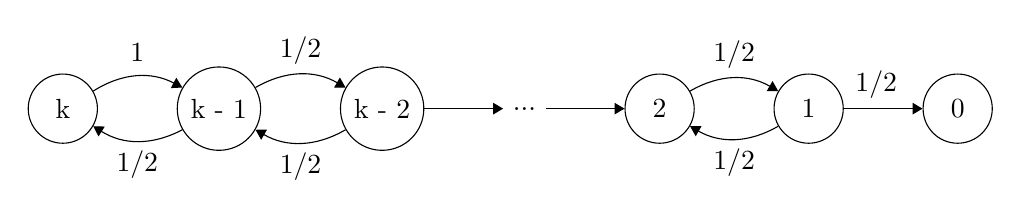
\begin{tikzpicture}[
   start chain = going right,
   -Triangle,
   every loop/.append style = {-Triangle}]
   \node[state, on chain]  (n) {k};
   \node[state, on chain]  (n1) {k - 1};
   \node[state, on chain]  (n2) {k - 2};
   \node[state without output/.append style={draw=none}, on chain]  (dots1) {...};
   \node[state, on chain]  (2) {2};
   \node[state, on chain]  (1) {1};
   \node[state, on chain]  (0) {0};

   \draw (n) edge[bend left] node[yshift=3mm]{$1$} (n1);
   \draw (n1) edge[bend left] node[yshift=-3mm]{$1/2$}(n);

   \draw (n1) edge[bend left] node[yshift=3mm]{$1/2$} (n2);
   \draw (n2) edge[bend left] node[yshift=-3mm]{$1/2$}(n1);

   \draw (n2) edge[left] node[xshift=3mm, yshift=-3mm]{} (dots1);

   \draw (dots1) edge[left] node[xshift=3mm, yshift=-3mm]{} (2);

  \draw (2) edge[bend left] node[yshift=3mm]{$1/2$} (1);
   \draw (1) edge[bend left] node[yshift=-3mm]{$1/2$}(2);

  \draw (1) edge[left] node[xshift=3mm, yshift=3mm]{$1/2$} (0);
\end{tikzpicture}
\caption{Embedded discrete Markov chain of the projected states of the $N$ node complete voter model.}
  \label{fig:rw_voter_model_discrete}
\end{figure}

\begin{lemma}\label{lem:rw_hit_zero}
Assume that we have a simple random walk on $\{0,1,\ldots, n\}$ where 0 is absorbing and $k$ is reflecting as shown in Figure \ref{fig:rw_voter_model_discrete}.
If we start in state $i \in \{1,\ldots, k - 1\}$, then the probability of hitting state 0 before state $n$ is $1/i$.
\end{lemma}

\begin{proof}
Let $A_j$ be the probability of hitting state 0 before state $n$ when starting from state $j \in \{1,\ldots, n - 1\}$ which is defined with the recurrence relations
\begin{align*}
    A_0 &= 1\\
    A_{n} &= 0\\
    A_j &= \frac{1}{2} A_{j + 1} + \frac{1}{2} A_{j - 1}
\end{align*}

The characteristic equation is $f(x) = x^2 - 2x + 1$ which has a double root at $1$.
Thus the solution of is of the form $A_j = a + bj$ and using the boundary conditions of $A_0 = 1$ and $A_{i} = 0$ we get
$$
A_j = \frac{n - j}{n}
$$
\end{proof}

\begin{theorem}
Assume that we have a simple random walk on $\{0,1,\ldots, k\}$ where 0 is absorbing and $k$ is reflecting as shown in Figure \ref{fig:rw_voter_model_discrete}.
Let $N_1, N_2, \ldots, N_k$ be the geometric random variables for the number of visits to each state.
Then,
$$
E[N_i] = \begin{cases}
    2i & 0 < i < k\\
    k & i = k
\end{cases}
$$
\end{theorem}

\begin{proof}
Using Lemma \ref{lem:rw_hit_zero} we have that for any $i \in \{1, \ldots, k - 1\}$ the probability of hitting 0 before hitting $i$ when starting in $i - 1$ is $\frac{1}{i}$.
Since we always return to $i$ if we move to $i + 1$, then the probability of never returning to $i$ is given by $\frac{1}{2i}$.
In the case when $i = k$, always go to the state $k - 1$ so the probability of never returning is simply $\frac{1}{k}$.
The result follow since the parameter in the geometric distribution is the probability of never returning to the state.
\end{proof}

\begin{theorem}
Let $\tau_{C_n^{v}}$ be the time until we reach state zero.
Now let $N_1, N_2, \ldots, N_k$ be the number of visits to states $1, 2, \ldots, k$ respectively, which are geometrically distributed.
Let $X_i^{(k)} \sim \exp(2k^2)$ be i.i.d random variables, $X_i^{(j)} \sim \exp(2i(n - i)\lambda)$ for each $j \in \{1, \ldots, k-1\}$ representing the exponential waiting time at each state.
We can represent $\tau_{C_n^{v}}$ as random sums

\begin{equation}\label{eq:wait_contact_sum}
    \tau_{C_n^{v}} = \sum_{i = 1}^{N_k} X_i^{(k)} + \sum_{i = 1}^{N_{k - 1}} X_i^{(k - 1)} + \cdots + \sum_{i = 1}^{N_1} X_i^{(1)}
\end{equation}
\end{theorem}


\subsection{Four node cycle \texorpdfstring{$S^{v}_4$}{VS4}}
State $2t$ is the configurations with the two matching values together such as $\{1100\}$ and $2s$ is the configuration with matching values apart such as $\{0101\}$

\begin{figure}[H]
    \centering
   %\begin{tikzpicture}[auto, node distance=2cm, every loop/.style={-Triangle}, thick,main node/.style={circle,draw}]
  \begin{tikzpicture}[start chain = going right,
   -Triangle, every loop/.append style = {-Triangle}]
   \node[state, on chain]  (1) {1};
   \node[state, on chain]  (2s) [left of=1, yshift = -10mm, xshift = -20mm]  {2s};

   \node[state, on chain]  (2t) [left of=1, yshift = 10mm, xshift = -20mm]  {2t};

   \node[state, on chain]  (0) [right of=1]  {0};

    \draw (2t) edge [bend left] node[yshift=3mm, xshift=1mm]{$2$} (1);
    \draw (1) edge [] node[yshift=-2mm, xshift=-1mm]{$1$} (2t);
    
    \draw (2s) edge [] node[yshift=-3.5mm, xshift=1mm]{$4$} (1);
    
    \draw (1) edge [] node[yshift=-2mm, xshift=-1mm]{$1$} (0);
    
%   \draw (111) edge [bend left] node[yshift=3.5mm, xshift=-1mm]{$2$} (110);
%   \draw (110) edge [] node[yshift=-2mm, xshift=1.5mm]{$\lambda$} (111);

%   \draw (111) edge [bend right] node[yshift=-3mm]{$1$} (101);
%   \draw (101) edge [] node[yshift=1.5mm, xshift = 2mm]{$2\lambda$} (111);

%   \draw (110) edge [bend left] node[yshift=3mm]{$1$} (010);
%   \draw (010) edge [] node[yshift=-2mm, xshift=1.5mm]{$2 \lambda$} (110);

%   \draw (101) edge [] node[yshift=-3mm]{$2$} (100);

%   \draw (110) edge [] node[yshift=3mm]{$1$} (100);
%   \draw (100) edge [bend left] node[yshift=3mm]{$\lambda$} (110);

%   \draw (010) edge [] node[yshift=3mm]{$1$} (000);
%   \draw (100) edge [] node[yshift=-3mm]{$1$} (000);

\end{tikzpicture}
    \caption{Projected rates of the four node voter model on cycle. State $2t$ are the configurations with the two matching values together such as $\{1100\}$ and $2s$ are the configurations with matching values apart such as $\{0101\}$}
    \label{fig:four_node_voter_cycle_rates}
\end{figure}

% Is it possible that we can use Burnside Polya counting (group actions) to show how many different distinct cycle configurations we get?

\subsection{Simulation of Linear Voter Model on \texorpdfstring{$\Z^2$}{Z2}}

The behavior of the linear voter model can be described as each voter waits exponential time and then takes the opinion of one of its neighbors according to the transition probabilities.
Assume that we are simulating on a $N \times N$ grid.
Using the exponential scaling property, this behavior is equivalent to waiting exponential time with rate $N^2$ and selecting a voter at random and updating their opinion.

\clearpage
\bibliographystyle{plainnat}
\bibliography{references}
\end{document}
